\documentclass[a4paper]{scrartcl}

\usepackage[
fancytheorems,
fancyproofs,
noindent,
]{adam}

\usepackage{tikz}
\usetikzlibrary{arrows, positioning, calc, decorations.pathreplacing}
\usepackage{bbm}
\usepackage{bm}
\usepackage{mathtools}

\newcommand{\WW}{\mathbb{W}}
\newcommand{\KK}{\mathbb{K}}
\newcommand{\dom}{\operatorname{dom}}
\newcommand{\Fin}{\operatorname{Fin}}
\newcommand{\Instr}{\operatorname{Instr}}
\newcommand{\code}{\operatorname{code}}
\newcommand{\graft}{\operatorname{graft}}
\newcommand{\lang}{\mathcal{L}}
\newcommand{\der}{\mathcal{D}}
\newcommand{\eps}{\varepsilon}
\newcommand{\Emp}{\mathbf{Emp}}
\newcommand{\Tot}{\mathbf{Tot}}
\newcommand{\Inf}{\mathbf{Inf}}
\newcommand{\Fine}{\mathbf{Fin}}
\newcommand{\Eq}{\mathbf{Eq}}

% Automaton drawing macros. A state is a circle; an accepting state is a
% double circle; transitions are thin arrows with a small label.
\tikzset{
  sta/.style={circle, draw, thick, minimum size=9mm, inner sep=2pt, font=\small},
  acc/.style={sta, double, double distance=1.1pt},
  tra/.style={->, >=stealth, thick, shorten >=1pt},
  tlab/.style={font=\footnotesize, inner sep=2.5pt},
  blob/.style={draw, thick, rounded corners=6pt},
  reg/.style={draw, thick, minimum width=8mm, minimum height=6mm, inner sep=0pt, font=\small}
}
% \initarr{node}{direction}: the incoming arrow marking the start state.
\newcommand{\initarr}[2]{\draw[tra] ($(#1)+#2$) -- (#1);}

\title{Automata and Formal Languages}
\author{Adam Kelly (\texttt{ak2316@cam.ac.uk})}
\date{\today}

\allowdisplaybreaks

\begin{document}

\maketitle

We all know an algorithm when we see one, and for most of mathematics that is enough. But some questions cannot be answered without saying exactly what an algorithm \emph{is}: if we want to prove that no algorithm solves a certain problem, we have to quantify over all possible algorithms, and to do that we need a definition. This course provides one -- in fact several, which turn out to agree -- and then uses it to show that a great many natural problems have no algorithmic solution at all.

Running alongside this is the theory of \emph{formal languages}. A language here is just a set of finite strings over a fixed alphabet, and this is a flexible enough notion to encode almost anything: sets of numbers, sets of graphs, sets of programs. Chomsky's insight was that languages come in a hierarchy, graded by how complicated a machine is needed to recognise them, and much of what follows is an exploration of the bottom two levels of that hierarchy -- the regular languages, recognised by finite automata, and the context-free languages, recognised by automata with a stack -- before we climb to the top and meet the languages recognised by a genuinely general-purpose computer.

This article constitutes my notes for the `Automata and Formal Languages' course, held in Michaelmas 2022 at Cambridge. These notes are \emph{not a transcription of the lectures}, and differ significantly in quite a few areas. Still, all lectured material should be covered.

\tableofcontents

\section{Introduction}

\subsection{Algorithms and the Entscheidungsproblem}

There is a difference between knowing that something exists and being able to find it. Compare the two statements
\begin{center}
`every polynomial of degree $n \geq 1$ over $\C$ has a root'
\end{center}
and
\begin{center}
`there is a procedure which, given such a polynomial, produces a root'.
\end{center}
The first is the fundamental theorem of algebra. The second is a genuinely different assertion, and there are plenty of situations in mathematics where the existence proof is available but no procedure is.

Historically, the demand for procedures came from Hilbert. In his 1900 address in Paris he set out a list of problems for the coming century, the tenth of which asks for a procedure which, given a Diophantine equation (a polynomial with integer coefficients), decides whether it has an integer solution. In 1928, in the book \emph{Grundz\"uge der theoretischen Logik} of Hilbert and Ackermann, the \vocab{Entscheidungsproblem} (`decision problem') was posed: give a procedure which, given a formula of predicate logic, decides whether it is a tautology.

In both cases Hilbert expected a positive answer, and here is the crucial asymmetry. To answer such a question positively one does not need a definition of `algorithm' at all: one simply writes an algorithm down, and everyone agrees on seeing it that it is one. To answer it negatively, one must rule out every conceivable algorithm, and for that a precise definition is unavoidable. Both of Hilbert's questions turned out to have negative answers -- Church and Turing settled the Entscheidungsproblem in 1936, and Matiyasevich settled the tenth problem in 1970 -- and neither answer could have been given before the work we do in this course.

\subsection{Alphabets, Words and Languages}

What are the objects on which computation is performed? One's first guess is `numbers', but neither of the two problems above has numbers as its input: one takes polynomials and the other takes formulae. What is common to them is that the inputs can be written down as finite strings of symbols drawn from a fixed finite stock. This is how all modern computation works, and it is the setting we adopt.

\begin{definition}[Strings]
	Let $\Omega$ be a set, whose elements we call \vocab{symbols}. For $n \in \N$ we write $\Omega^n$ for the set of functions $n \to \Omega$, thinking of the natural number $n$ as the set $\{0, 1, \dots, n-1\}$ in the usual von Neumann way, so that an element of $\Omega^n$ is a sequence $(x_0, \dots, x_{n-1})$ of symbols. We write
	$$\Omega^\star = \bigcup_{n \in \N} \Omega^n$$
	for the set of all finite sequences of symbols, which we call \vocab{$\Omega$-strings}.
\end{definition}

We will suppress the sequence notation entirely and write strings by juxtaposition, so that $(x_0, x_1, x_2)$ is written $x_0x_1x_2$. The following conventions will be used without comment.
\begin{itemize}
	\item The \vocab{length} of a string $\alpha \in \Omega^n$ is $\abs{\alpha} = n$.
	\item $\Omega^0$ has exactly one element, the \vocab{empty string} $\eps$.
	\item Given $\alpha \in \Omega^n$ and $k \leq n$, the \vocab{truncation} $\alpha\restriction_k$ is the unique element of $\Omega^k$ which is an initial segment of $\alpha$.
	\item Given $\alpha \in \Omega^m$ and $\beta \in \Omega^n$, their \vocab{concatenation} $\alpha\beta \in \Omega^{m+n}$ is defined in the obvious way. Concatenation is associative with identity $\eps$, so $\Omega^\star$ is a monoid.
	\item We define $\alpha^0 = \eps$ and $\alpha^{n+1} = \alpha\alpha^n$.
	\item We identify a symbol $x \in \Omega$ with the string of length one that it determines.
	\item If $Y, Z \subseteq \Omega^\star$ then $YZ = \{\alpha\beta \mid \alpha \in Y,\, \beta \in Z\}$, and if $Y = \{\alpha\}$ we simply write $\alpha Z$.
	\item A function $f \colon \Omega \to \Omega'$ lifts to a function $\Omega^\star \to \Omega'^\star$ acting symbolwise; we write this lift as $f$ as well.
\end{itemize}

Now, not every string is a sensible object. If $\Omega$ is a stock of letters then $\Omega^\star$ contains a great many strings which are not words of English; if $\Omega$ is a stock of words then $\Omega^\star$ contains a great many strings which are not sentences. So we will want to designate a subset of $\Omega^\star$ as the \emph{well-formed} strings, and it is these subsets which are the objects of study.

\begin{definition}[Alphabet, word, language]
	An \vocab{alphabet} is a finite nonempty set $\Sigma$, whose elements we call \vocab{letters} and denote $a, b, c, \dots$. We write
	$$\WW = \Sigma^\star$$
	for the set of \vocab{words}, denoted $u, v, w, \dots$, and $\WW^+ = \WW \setminus \{\eps\}$ for the set of nonempty words. A \vocab{language} over $\Sigma$ is a subset $L \subseteq \WW$.
\end{definition}

Because a language is simply a set of words, and words can encode anything, this is a very general notion indeed. The set of prime numbers written in binary is a language over $\{0,1\}$; so is the set of (codes of) computer programs that never terminate. The whole of this course can be read as the study of how complicated a language can be.

\subsection{Counting Languages}

We record here some counting facts from Numbers and Sets which will be used repeatedly, usually to demonstrate that some class of languages cannot possibly contain all of them. Recall that $X$ is \vocab{countable} if there is a surjection $\N \to X$ (or $X = \varnothing$), and that $X$ is \vocab{infinite} if there is an injection $\N \to X$.

\begin{proposition}\label{prop:starcountable}
	If $X$ is nonempty and countable then $X^\star$ is countably infinite.
\end{proposition}

\begin{proof}
	Pick $x \in X$. The map $n \mapsto x^n$ is an injection $\N \to X^\star$, so $X^\star$ is infinite.

	For countability, let $\pi \colon \N \to X$ be a surjection. Every $k \in \N$ with $k > 0$ has a unique prime factorisation $k = \prod_{i} p_i^{k_i}$, where $p_0 = 2, p_1 = 3, p_2 = 5, \dots$ enumerates the primes. Read $k_0$ as a length and send $k$ to the string
	$$\pi(k_1)\,\pi(k_2)\cdots\pi(k_{k_0}) \in X^\star,$$
	sending $0$ to $\eps$ as well. Given any string $\alpha = y_1\cdots y_n \in X^\star$, choose $m_j$ with $\pi(m_j) = y_j$ and take $k = 2^n 3^{m_1} 5^{m_2} \cdots$; this maps onto $\alpha$. So the map is a surjection $\N \to X^\star$.
\end{proof}

\begin{proposition}\label{prop:fincountable}
	If $X$ is countable then the set $\Fin(X)$ of finite subsets of $X$ is countable.
\end{proposition}

\begin{proof}
	The `forgetful' map $X^\star \to \Fin(X)$ sending $y_1\cdots y_n$ to $\{y_1, \dots, y_n\}$ is a surjection: given a finite $F \subseteq X$, list its elements in any order. Composing with the surjection of Proposition~\ref{prop:starcountable} gives a surjection $\N \to \Fin(X)$.
\end{proof}

On the other hand, by Cantor's theorem $\power(X)$ is uncountable whenever $X$ is infinite. Since $\WW$ is countably infinite, we obtain the following, which is the first thing worth knowing about languages.

\begin{corollary}\label{cor:uncountablymanylanguages}
	There are uncountably many languages over any alphabet.
\end{corollary}

Every method we shall meet for \emph{specifying} a language -- a grammar, an automaton, a regular expression, a register machine -- is a finite object over some finite alphabet, and so there are only countably many of them. Consequently \emph{every} such method fails to describe almost every language. This is not a defect of any particular formalism; it is a fact about cardinality, and it is worth keeping in mind throughout.

\section{Rewrite Systems and Grammars}

\subsection{Rewrite Systems}

The most primitive way of generating strings is to start with one and repeatedly replace pieces of it. This is the notion of a rewrite system, and everything in the first half of the course is a special case of it.

\begin{definition}[Rewrite system]
	Let $\Omega$ be a finite set of symbols. An element $(\alpha, \beta)$ of $\Omega^\star \times \Omega^\star$ is called a \vocab{rewrite rule} or \vocab{production rule}, and is written $\alpha \to \beta$. A pair $R = (\Omega, P)$ is a \vocab{rewrite system} if $P$ is a \emph{finite} set of rewrite rules.
\end{definition}

The intended reading of $\alpha \to \beta$ is `wherever you see $\alpha$, you may replace it by $\beta$'. Let us make that precise.

\begin{definition}[Derivation]
	Let $R = (\Omega, P)$ be a rewrite system and let $\sigma, \tau \in \Omega^\star$. We write
	$$\sigma \Rightarrow_R \tau$$
	and say that \vocab{$R$ produces $\tau$ from $\sigma$ in one step}, if there are $\alpha, \beta, \gamma, \delta \in \Omega^\star$ with $\sigma = \alpha\gamma\beta$, $\tau = \alpha\delta\beta$ and $\gamma \to \delta \in P$. We write $\Rightarrow_R^\star$ for the reflexive transitive closure of $\Rightarrow_R$. A sequence
	$$\sigma_0 \Rightarrow_R \sigma_1 \Rightarrow_R \cdots \Rightarrow_R \sigma_n$$
	is an \vocab{$R$-derivation of $\sigma_n$ from $\sigma_0$ of length $n$}, and we write
	$$\der(R, \sigma) = \{\tau \in \Omega^\star \mid \sigma \Rightarrow_R^\star \tau\}$$
	for the set of strings derivable from $\sigma$.
\end{definition}

Note that $\alpha$ and $\beta$ here are the \emph{context} in which the rewriting takes place; the rule fires regardless of what surrounds the occurrence of $\gamma$. We will meet later a restricted notion in which the context is allowed to constrain the rule, and this is the origin of the word `context-free'.

Since a rewrite system is a finite object over a finite alphabet, Propositions~\ref{prop:starcountable} and~\ref{prop:fincountable} give the following immediately.

\begin{proposition}
	For fixed finite $\Omega$, there are only countably many rewrite systems on $\Omega$.
\end{proposition}

\begin{proof}
	$\Omega^\star$ is countable, hence so is $\Omega^\star \times \Omega^\star$, hence so is $\Fin(\Omega^\star \times \Omega^\star)$, and every $P$ lies in the latter.
\end{proof}

\subsection{Grammars}

The application we care about is to languages. Chomsky's idea was that a natural language should be modelled not by a finite list of well-formed sentences, but by a finite list of \emph{rules} which generate infinitely many sentences. The reason for insisting on infinitude is \vocab{linguistic recursion}: if $X$ is a grammatical English sentence then so is `Alice believes that $X$', and if we impose a maximum sentence length we are obliged to cut this off at some arbitrary point.

Here is a toy example of the sort of thing Chomsky had in mind. Take the rules
\begin{align*}
	S &\to \text{NP VP}, & \text{NP} &\to \text{Adj NP}, & \text{NP} &\to \text{Noun}, \\
	\text{VP} &\to \text{Verb}, & \text{VP} &\to \text{Verb Adv},
\end{align*}
together with rules turning $\text{Adj}$ into an adjective, $\text{Noun}$ into a noun and so on. Starting from $S$ one can derive `colourless green ideas sleep furiously', Chomsky's famous example of a sentence that is grammatical but meaningless; one cannot derive `furiously sleep ideas green colourless', which is neither. The moral is that grammaticality is a formal, checkable property, whereas meaningfulness is not something a rewrite system can see.

The symbols in this example fall into two classes: those like $S$ and NP which are scaffolding, and those like `ideas' which are part of the final product. This distinction is built into the definition.

\begin{definition}[Grammar]
	Let $\Sigma$ be an alphabet and let $V$ be a nonempty finite set disjoint from $\Sigma$, whose elements we call \vocab{variables} or \vocab{nonterminal symbols}, denoted $A, B, C, \dots$. Write $\Omega = \Sigma \cup V$. A \vocab{grammar} is a tuple $G = (\Sigma, V, P, S)$ where $(\Omega, P)$ is a rewrite system and $S \in V$ is the \vocab{start symbol}.

	We use the notation for rewrite systems for the associated rewrite system, writing $\Rightarrow_G$, $\Rightarrow_G^\star$ and $\der(G, \sigma)$. The \vocab{language generated by $G$} is
	$$\lang(G) = \der(G, S) \cap \WW.$$
\end{definition}

So a word lies in $\lang(G)$ exactly when it can be derived from the start symbol and contains no variables. Two easy ways for this to fail are worth noting straight away.

\begin{example}
	If $P$ contains no rule of the form $S \to \alpha$, then $\der(G,S) = \{S\}$, which contains no words, so $\lang(G) = \varnothing$. Similarly, if no rule has a right-hand side lying in $\WW$, then nothing in $\der(G,S)$ can be a word, and again $\lang(G) = \varnothing$.
\end{example}

\begin{example}\label{ex:oddas}
	Let $\Sigma = \{a\}$, $V = \{S\}$ and $P_0 = \{S \to aaS,\; S \to a\}$. We claim that
	$$\lang(G_0) = \{a^{2n+1} \mid n \in \N\}.$$
	Each rule replaces a string by one of length two greater, or of the same length, so by induction on the length of a derivation every element of $\der(G_0, S)$ has odd length; in particular every word produced is $a^{2n+1}$ for some $n$. Conversely, applying $S \to aaS$ exactly $n$ times and then $S \to a$ produces $a^{2n+1}$.

	Observe that the only feature of $P_0$ used in the argument was that every rule preserves the parity of the length. So the rule sets
	\begin{align*}
		P_1 &= \{S \to aSa,\; S \to a\}, & P_2 &= \{S \to Saa,\; S \to a\}, \\
		P_3 &= \{S \to aaS,\; S \to aaSaa,\; S \to a\}
	\end{align*}
	all generate the same language. Different grammars can generate the same language, and this is the phenomenon we look at next.
\end{example}

\subsection{Equivalence of Grammars}

\begin{definition}[Equivalent grammars]
	Grammars $G$ and $G'$ over the same alphabet are \vocab{equivalent} if $\lang(G) = \lang(G')$.
\end{definition}

Our aim in this subsection is to show that, for a fixed alphabet $\Sigma$, there are only countably many languages of the form $\lang(G)$. The point requiring care is that $V$ is allowed to be an arbitrary finite set, so there is a proper class of grammars to begin with; we must cut this down to a set. The tool is the observation that the names of the variables do not matter.

\begin{definition}[Isomorphism of grammars]
	Let $G = (\Sigma, V, P, S)$ and $G' = (\Sigma, V', P', S')$ be grammars over the same alphabet. A function $f \colon \Omega \to \Omega'$ is an \vocab{isomorphism} if
	\begin{enumerate}[label=(\roman*)]
		\item $f\restriction_\Sigma = \mathrm{id}$;
		\item $f(S) = S'$;
		\item $f\restriction_V$ is a bijection $V \to V'$;
		\item $\alpha \to \beta \in P$ if and only if $f(\alpha) \to f(\beta) \in P'$,
	\end{enumerate}
	where in (iv) we use the lift of $f$ to $\Omega^\star$.
\end{definition}

\begin{proposition}
	Isomorphic grammars are equivalent.
\end{proposition}

\begin{proof}
	If $f$ is an isomorphism $G \to G'$ then $f^{-1}$ is an isomorphism $G' \to G$, so it suffices to prove $\lang(G) \subseteq \lang(G')$. Let $w \in \lang(G)$, with derivation
	$$S = \sigma_0 \Rightarrow_G \sigma_1 \Rightarrow_G \cdots \Rightarrow_G \sigma_n = w.$$
	Apply $f$ throughout. By (ii) the first term is $S'$; by (i) the last term is still $w$, since $w$ contains only letters; and by (iv) each single step remains a legal step, since the decomposition $\sigma_i = \alpha\gamma\beta$ maps to $f(\sigma_i) = f(\alpha)f(\gamma)f(\beta)$. So $S' \Rightarrow_{G'}^\star w$ and $w \in \lang(G')$.
\end{proof}

\begin{proposition}\label{prop:relabel}
	Let $G = (\Sigma, V, P, S)$ be a grammar and let $V'$ be any set with $\abs{V} = \abs{V'}$ and $V' \cap \Sigma = \varnothing$. Then there are $P'$ and $S'$ with $G' = (\Sigma, V', P', S')$ equivalent to $G$.
\end{proposition}

\begin{proof}
	Choose a bijection $f \colon V \to V'$ and extend it to $\Omega$ by the identity on $\Sigma$, so that (i) and (iii) hold. Set $S' = f(S)$ and $P' = \{f(\alpha) \to f(\beta) \mid \alpha \to \beta \in P\}$, so that (ii) and (iv) hold. Then $G \cong G'$, so the two are equivalent.
\end{proof}

\begin{proposition}\label{prop:countablymanygrammarlanguages}
	For a fixed alphabet $\Sigma$, there are only countably many languages of the form $\lang(G)$ for a grammar $G$.
\end{proposition}

\begin{proof}
	Fix a finite set $V$ disjoint from $\Sigma$. There are only countably many rewrite systems on $\Omega = \Sigma \cup V$, and only finitely many choices of start symbol, so the collection $\mathcal{G}_V$ of grammars with this variable set is countable, and hence so is $\mathcal{L}_V = \{\lang(G) \mid G \in \mathcal{G}_V\}$.

	By Proposition~\ref{prop:relabel}, $\mathcal{L}_V$ depends only on $\abs{V}$, so we may write $\mathcal{L}_n$ for the value at any $n$-element $V$, and every language generated by a grammar lies in some $\mathcal{L}_n$. Then $\bigcup_{n > 0} \mathcal{L}_n$ is a countable union of countable sets and is therefore countable.
\end{proof}

Combining this with Corollary~\ref{cor:uncountablymanylanguages}, almost every language is generated by no grammar at all. Grammars are nevertheless the right thing to study, because the languages they generate are exactly the ones we can hope to compute with; we shall see in Section~\ref{sec:re} that they are precisely the \emph{computably enumerable} languages.

\subsection{The Chomsky Hierarchy}

Restricting the \emph{shape} of the allowed production rules restricts the languages that can be generated, and Chomsky's classification is obtained by imposing four increasingly severe such restrictions.

\begin{definition}[Types of production rule]
	Let $\alpha \to \beta$ be a production rule. We call it
	\begin{enumerate}[label=(\roman*)]
		\item \vocab{noncontracting} if $\abs{\alpha} \leq \abs{\beta}$;
		\item \vocab{context-sensitive} if there are $A \in V$, $\gamma, \delta \in \Omega^\star$ and $\eta \in \Omega^\star$ with $\abs{\eta} > 0$ such that $\alpha = \gamma A \delta$ and $\beta = \gamma\eta\delta$;
		\item \vocab{context-free} if $\alpha = A \in V$ and $\abs{\beta} > 0$;
		\item \vocab{regular} if $\alpha = A \in V$ and $\beta$ is either $a$ or $aB$ for some $a \in \Sigma$ and $B \in V$.
	\end{enumerate}
	A grammar has one of these properties if all of its rules do, and a language has one of these properties if it is generated by some grammar which has it.
\end{definition}

A context-sensitive rule may replace $A$ by $\eta$, but only when $A$ occurs in the context $\gamma \_\, \delta$; the surrounding material is not allowed to change. A context-free rule may replace $A$ by $\beta$ wherever it occurs. A regular rule may only replace a variable by a letter, or by a letter followed by a single variable, so that a derivation grows strictly from left to right.

Immediately from the definitions, regular $\Rightarrow$ context-free $\Rightarrow$ context-sensitive $\Rightarrow$ noncontracting. (For the middle implication, take $\gamma = \delta = \eps$.) In Chomsky's numbering, a language $L$ is
\begin{itemize}
	\item \vocab{type 0} if $L = \lang(G)$ for some grammar $G$;
	\item \vocab{type 1} if $L = \lang(G)$ for some context-sensitive $G$;
	\item \vocab{type 2} if $L = \lang(G)$ for some context-free $G$;
	\item \vocab{type 3} if $L = \lang(G)$ for some regular $G$.
\end{itemize}

\begin{center}
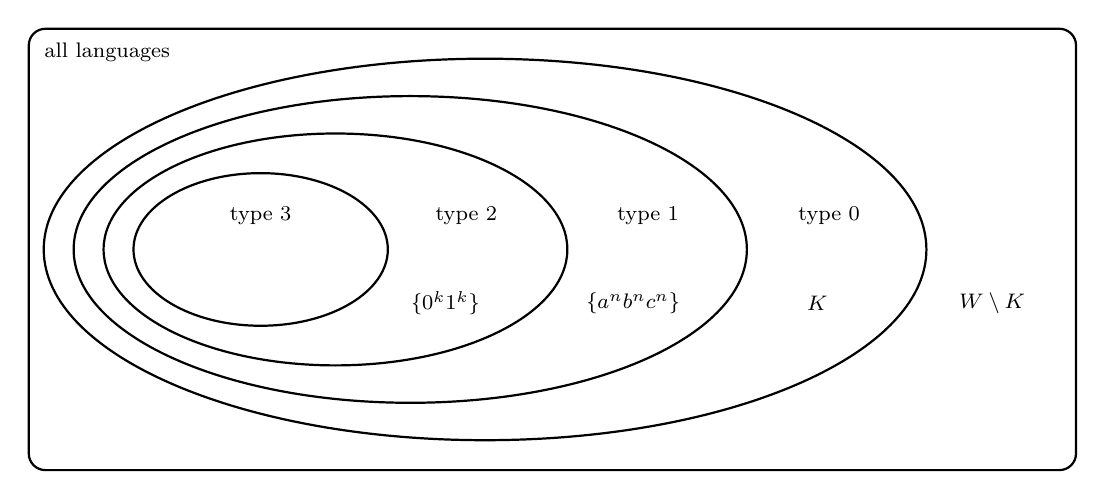
\begin{tikzpicture}[scale=0.95, transform shape,
	lbl/.style={font=\footnotesize, fill=white, inner sep=1.5pt}]
	\draw[blob] (-7.0,-2.95) rectangle (7.0,2.95);
	\draw[thick] (-0.9,0) ellipse (5.9 and 2.55);
	\draw[thick] (-1.9,0) ellipse (4.5 and 2.05);
	\draw[thick] (-2.9,0) ellipse (3.1 and 1.55);
	\draw[thick] (-3.9,0) ellipse (1.7 and 1.02);
	\node[lbl] at (-3.90,0.45) {type $3$};
	\node[lbl] at (-1.15,0.45) {type $2$};
	\node[lbl] at (1.28,0.45) {type $1$};
	\node[lbl] at (3.70,0.45) {type $0$};
	\node[lbl, anchor=west] at (-6.85,2.63) {all languages};
	\node[lbl] at (-1.43,-0.72) {$\{0^k1^k\}$};
	\node[lbl] at (1.08,-0.72) {$\{a^nb^nc^n\}$};
	\node[lbl] at (3.54,-0.72) {$\KK$};
	\node[lbl] at (5.88,-0.72) {$\WW \setminus \KK$};
\end{tikzpicture}
\end{center}

The picture is the one to keep in mind, and proving that the inclusions are all strict -- that the sample languages really do sit where they are drawn -- occupies a large part of the course. We will show that $\{0^k1^k \mid k > 0\}$ is context-free but not regular, and that $\{a^nb^nc^n \mid n > 0\}$ is context-sensitive but not context-free; the halting set $\KK$ and its complement will be dealt with in Section~\ref{sec:re}.

The following theorem of Chomsky says that two of our four conditions define the same class of languages, even though they do not define the same class of grammars. We shall not prove it.

\begin{theorem}[Chomsky]
	A language is noncontracting if and only if it is context-sensitive.
\end{theorem}

\subsection{Decision Problems}

Alongside the question `which languages arise?' we ask `what can we work out about them?'. Three questions will accompany us throughout.

\begin{definition}[The three decision problems]
	\begin{enumerate}[label=(\roman*)]
		\item The \vocab{word problem} takes as input a grammar $G$ and a word $w$, and asks whether $w \in \lang(G)$.
		\item The \vocab{emptiness problem} takes as input a grammar $G$ and asks whether $\lang(G) = \varnothing$.
		\item The \vocab{equivalence problem} takes as input grammars $G$ and $G'$ and asks whether $\lang(G) = \lang(G')$.
	\end{enumerate}
	A problem is \vocab{solvable} if there is an algorithm giving the correct answer for every input, and \vocab{unsolvable} otherwise.
\end{definition}

For the moment `algorithm' is informal; in Section~\ref{sec:solvability} we will replace it by a precise definition and revisit all three problems. It will turn out that all three are unsolvable for grammars in general. Lower down the hierarchy things are better, and we can already deal with the word problem.

\begin{lemma}\label{lem:wordproblembound}
	Let $G$ be a noncontracting grammar and let $w \in \WW$. There is a bound $N$, depending only on $\abs{w}$ and $\abs{\Omega}$, such that $w \in \lang(G)$ if and only if $w$ has a $G$-derivation of length at most $N$.
\end{lemma}

\begin{proof}
	Let $S = \sigma_0 \Rightarrow_G \cdots \Rightarrow_G \sigma_n = w$ be a derivation of minimal length. As $G$ is noncontracting, the sequence of lengths $1 = \abs{\sigma_0} \leq \abs{\sigma_1} \leq \cdots \leq \abs{\sigma_n} = \abs{w}$ is nondecreasing. If $\sigma_r = \sigma_s$ for some $r < s$ then deleting $\sigma_{r+1}, \dots, \sigma_s$ leaves a shorter derivation, so by minimality all the $\sigma_i$ are distinct. But every $\sigma_i$ is a string over $\Omega$ of length at most $\abs{w}$, and there are only
	$$N = \sum_{\ell = 1}^{\abs{w}} \abs{\Omega}^\ell$$
	of these, so $n \leq N$ by pigeonhole.
\end{proof}

\begin{corollary}\label{cor:wordproblemsolvable}
	The word problem is solvable for noncontracting, context-sensitive, context-free and regular grammars.
\end{corollary}

\begin{proof}
	Given $G$ and $w$, compute $N$ as above. There are only finitely many derivations of length at most $N$, since at each step only finitely many rules can be applied at finitely many positions, and they can be enumerated; check each one.
\end{proof}

This is a good illustration of the difference between solvability and practicality. The bound $N$ is astronomically large, and the algorithm above is of no practical use whatsoever; but solvability is a statement about existence, and existence is what we get.

\subsection{Closure Properties}

The other standard question about a class of languages is which operations it is closed under. Given languages $L$ and $M$ over $\Sigma$, the operations of interest are
$$LM, \quad L \cup M, \quad L \cap M, \quad L \setminus M, \quad \WW^+ \setminus L.$$
We use $\WW^+ \setminus L$ rather than $\WW \setminus L$ for the complement, because (as we check below) a noncontracting grammar can never produce $\eps$, so no class below type 0 could possibly be closed under an operation that introduces the empty word.

Some closure properties come for free from others: for instance, closure under complement and union implies closure under intersection, by De Morgan.

\begin{definition}[Union and concatenation grammars]
	Let $G = (\Sigma, V, P, S)$ and $G' = (\Sigma, V', P', S')$ be grammars, and let $T$ be a variable in neither $V$ nor $V'$. The \vocab{concatenation grammar} is
	$$H = (\Sigma,\, V \cup V' \cup \{T\},\, P \cup P' \cup \{T \to SS'\},\, T),$$
	and the \vocab{union grammar} is
	$$H' = (\Sigma,\, V \cup V' \cup \{T\},\, P \cup P' \cup \{T \to S,\, T \to S'\},\, T).$$
\end{definition}

It is clear that $\lang(G)\lang(G') \subseteq \lang(H)$ and $\lang(G) \cup \lang(G') \subseteq \lang(H')$. The reverse inclusions, however, are \emph{not} automatic. Even after relabelling so that $V \cap V' = \varnothing$, the two rule sets can interact: a rule of $P$ whose left-hand side contains letters can fire on a string produced by $P'$. The way to rule this out is to arrange that no rule mentions a letter on its left.

\begin{definition}[Variable-based]
	A rule $\alpha \to \beta$ is \vocab{variable-based} if every symbol occurring in $\alpha$ is a variable, and a grammar is variable-based if all of its rules are.
\end{definition}

Regular and context-free grammars are automatically variable-based, since their rules have $\alpha = A \in V$. Context-sensitive grammars need not be.

\begin{lemma}\label{lem:variablebased}
	Every grammar is equivalent to a variable-based grammar. Moreover, if the original grammar is context-free, context-sensitive or noncontracting, then so is the new one.
\end{lemma}

\begin{proof}
	Let $G = (\Sigma, V, P, S)$. For each letter $a \in \Sigma$ introduce a fresh variable $X_a$, and let $X \colon \Omega \to \Omega$ send $a \mapsto X_a$ for $a \in \Sigma$ and fix $V$ pointwise; lift $X$ to $\Omega^\star$. Put
	$$P' = \{X(\alpha) \to X(\beta) \mid \alpha \to \beta \in P\}, \qquad P'' = \{X_a \to a \mid a \in \Sigma\},$$
	and let $G' = (\Sigma, V \cup \{X_a \mid a \in \Sigma\}, P' \cup P'', S)$. Every rule of $P'$ has only variables on the left by construction, and every rule of $P''$ has a single variable on the left, so $G'$ is variable-based. The added rules $X_a \to a$ are regular, so they preserve context-freeness, context-sensitivity and noncontraction.

	It remains to check $\lang(G) = \lang(G')$. Applying $X$ to a $G$-derivation of $w$ gives a $G'$-derivation of $X(w)$, and then applying the rules $X_a \to a$ once for each letter of $w$ gives $w$; so $\lang(G) \subseteq \lang(G')$.

	Conversely let $S = \sigma_0 \Rightarrow_{G'} \cdots \Rightarrow_{G'} \sigma_m = w$ be a $G'$-derivation. Apply $X$ to every term to get a sequence $\tau_0, \dots, \tau_m$ with $\tau_0 = S$ and $\tau_m = X(w)$. If the step $\sigma_i \Rightarrow_{G'} \sigma_{i+1}$ used a rule $X(\alpha) \to X(\beta)$, then since $X$ fixes such strings we still have $\tau_i \Rightarrow_{G'} \tau_{i+1}$ by the same rule, which is a rule of $G$ after erasing $X$. If instead it used a rule $X_a \to a$, then $\tau_i = \tau_{i+1}$, and we delete the repetition. Deleting all such repetitions leaves a genuine $G$-derivation of $w$ (after erasing $X$ throughout, which is legitimate since no string in the resulting sequence contains any $X_a$). Hence $w \in \lang(G)$.
\end{proof}

\begin{theorem}\label{thm:closureunionconcat}
	Let $G$ and $G'$ be variable-based grammars over $\Sigma$ with $V \cap V' = \varnothing$. Then
	$$\lang(H) = \lang(G)\lang(G'), \qquad \lang(H') = \lang(G) \cup \lang(G').$$
	Consequently the classes of context-free, context-sensitive and noncontracting languages are closed under union and concatenation, and the class of regular languages is closed under union.
\end{theorem}

\begin{proof}
	One inclusion in each case has already been observed. For the other, consider a derivation in $H$. The first step must be $T \to SS'$, since $T$ occurs in no other rule's right-hand side and appears nowhere else. Thereafter every rule applied has a variable-only left-hand side, so it lies entirely within the $V$-part or entirely within the $V'$-part of the string, these being disjoint. Thus the derivation splits into a $G$-derivation acting on the first component and a $G'$-derivation acting on the second, and any word produced is of the form $vw$ with $v \in \lang(G)$ and $w \in \lang(G')$. The argument for $H'$ is the same, the first step being $T \to S$ or $T \to S'$.

	For the closure statements, given two grammars of the relevant type we first pass to equivalent variable-based grammars with disjoint variable sets, using Lemma~\ref{lem:variablebased} and Proposition~\ref{prop:relabel}, and then apply the above. The union grammar of two regular grammars is not regular, because of the rules $T \to S$; we shall prove closure of the regular languages under union and concatenation by other means in Section~\ref{sec:regular}.
\end{proof}

\subsection{The Empty Word}

\begin{remark}
	No noncontracting grammar produces $\eps$: every string in a derivation from $S$ has length at least $\abs{S} = 1$. In particular no type $1$, $2$ or $3$ language contains the empty word, which is why $\WW^+$ rather than $\WW$ is the correct ambient set for those classes.
\end{remark}

One might hope simply to add the rule $S \to \eps$ to put $\eps$ into a language, but this can have side effects: if $S$ occurs on the right-hand side of some rule then the new rule can fire in the middle of a derivation and delete a symbol that was doing work.

\begin{definition}
	A rule $\alpha \to \beta$ is \vocab{$S$-safe} if $S$ does not occur in $\beta$. A grammar is \vocab{$\eps$-adequate} if all of its rules are $S$-safe.
\end{definition}

If $G$ is $\eps$-adequate then $S$ can only ever appear as the very first string of a derivation, so adding $S \to \eps$ produces a grammar for $\lang(G) \cup \{\eps\}$ and nothing else. Moreover every grammar is equivalent to an $\eps$-adequate one: replace $G = (\Sigma, V, P, S)$ by
$$G' = (\Sigma,\, V \cup \{T\},\, P \cup \{T \to S\},\, T)$$
for a fresh variable $T$. This will be used without comment whenever it is convenient.

\section{Regular Languages}\label{sec:regular}

The lowest level of the hierarchy is the most thoroughly understood, and it is where we start. We will see that regular languages admit four completely different descriptions -- by grammars, by deterministic automata, by nondeterministic automata, and by regular expressions -- and that all four are effectively interchangeable. We will also obtain a tool (the pumping lemma) for proving that a language is \emph{not} regular, and a canonical minimal automaton for each regular language.

\subsection{Regular Derivations}

Recall that a regular rule has the form $A \to a$ or $A \to aB$. We call the first kind \vocab{terminal} and the second kind \vocab{nonterminal}. The shape of regular derivations is extremely rigid, which is what makes the theory work.

\begin{lemma}\label{lem:regularform}
	Let $G$ be a regular grammar. If $S \Rightarrow_G^\star \alpha$ then $\alpha \in \WW \cup \WW V$; that is, $\alpha$ is a word, possibly followed by a single variable.
\end{lemma}

\begin{proof}
	Induction on the length of the derivation. The empty derivation gives $\alpha = S = \eps S \in \WW V$. Suppose $S \Rightarrow_G^\star \beta \Rightarrow_G \alpha$ with $\beta \in \WW \cup \WW V$. If $\beta \in \WW$ then $\beta$ contains no variable, but every rule rewrites a variable, so no step is possible; so $\beta = wA$ with $w \in \WW$, $A \in V$. The applicable rules are $A \to a$ and $A \to aB$, giving $\alpha = wa \in \WW$ or $\alpha = waB \in \WW V$ respectively.
\end{proof}

\begin{lemma}\label{lem:regularlength}
	Let $G$ be regular and $w \in \WW$ with $S \Rightarrow_G^\star w$. Then every derivation of $w$ from $S$ has length exactly $\abs{w}$, and consists of $\abs{w} - 1$ nonterminal rules followed by a single terminal rule.
\end{lemma}

\begin{proof}
	A nonterminal rule increases the length of the string by one and leaves the number of variables at one; a terminal rule leaves the length unchanged and reduces the number of variables from one to zero. Starting from $S$, of length $1$ with one variable, we therefore need exactly $\abs{w} - 1$ nonterminal steps to reach length $\abs{w}$. Once the variable count reaches zero no further rule applies, so the terminal rule must come last, and there is exactly one of them.
\end{proof}

Note that the derivation is nonetheless not \emph{unique}, since there may be several rules $A \to aB$ with the same $A$ and $a$. This is precisely the nondeterminism that we will have to deal with below.

As a first application, we can now handle concatenation, which Theorem~\ref{thm:closureunionconcat} did not give us for regular languages.

\begin{lemma}\label{lem:regconcat}
	Regular languages are closed under concatenation.
\end{lemma}

\begin{proof}
	Let $G = (\Sigma, V, P, S)$ and $G' = (\Sigma, V', P', S')$ be regular, with $V \cap V' = \varnothing$ after relabelling. Let $P^\star$ be obtained from $P$ by replacing every terminal rule $A \to a$ by the nonterminal rule $A \to aS'$, and set $H = (\Sigma, V \cup V', P^\star \cup P', S)$. This is regular. We claim $\lang(H) = \lang(G)\lang(G')$.

	If $S \Rightarrow_G^\star v$ and $S' \Rightarrow_{G'}^\star w$, then running the $G$-derivation in $H$ and using the modified last rule yields $S \Rightarrow_H^\star vS'$, and then the $G'$-derivation gives $S \Rightarrow_H^\star vw$.

	Conversely suppose $S \Rightarrow_H^\star u$ with $u \in \WW$. By Lemma~\ref{lem:regularform} every intermediate string is $w_iX_i$ with $X_i \in V \cup V'$. Initially $X_0 = S \in V$. The only rules taking a variable of $V$ to a variable of $V'$ are the modified rules $A \to aS'$, and no rule of $P'$ mentions a variable of $V$; so once the derivation enters $V'$ it stays there. Splitting the derivation at the unique step where this happens gives $u = vw$ with $S \Rightarrow_G^\star v$ (using the original terminal rule in place of the modified one) and $S' \Rightarrow_{G'}^\star w$.
\end{proof}

\subsection{Deterministic Automata}

We now come to the machine model. A deterministic automaton reads a word one letter at a time, from left to right, keeping track of nothing except which of finitely many states it is in.

\begin{definition}[Deterministic automaton]
	Let $\Sigma$ be an alphabet. A \vocab{deterministic automaton} is a tuple $D = (\Sigma, Q, \delta, q_0, F)$ where $Q$ is a finite set of \vocab{states}, $q_0 \in Q$ is the \vocab{start state}, $F \subseteq Q \setminus \{q_0\}$ is the set of \vocab{accept states}, and $\delta \colon Q \times \Sigma \to Q$ is the \vocab{transition function}.
\end{definition}

The requirement $q_0 \notin F$ is a convention forced on us by the fact that regular grammars cannot generate $\eps$; it will mean that $\eps$ never lies in the language of an automaton, matching the grammar side exactly. It is a harmless restriction, and we will return to it when we discuss the Kleene star.

We draw an automaton as a labelled directed graph: one node per state, drawn as a circle, or as a double circle if the state is accepting; an unlabelled incoming arrow marks the start state; and for each $q$ and $a$ there is an arrow from $q$ to $\delta(q,a)$ labelled $a$. Every node therefore has exactly $\abs{\Sigma}$ outgoing arrows, though several may be drawn as one arrow with several labels.

\begin{example}\label{ex:atleastonezero}
	Let $\Sigma = \{0,1\}$ and consider the following automaton.
	\begin{center}
	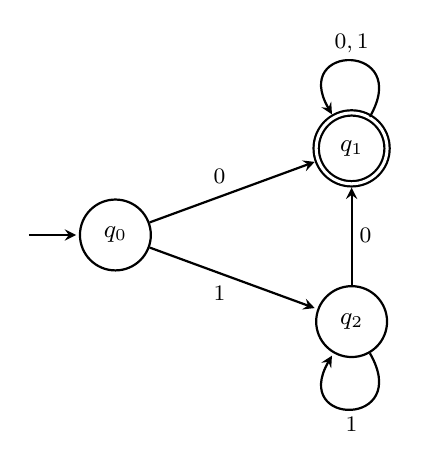
\begin{tikzpicture}
		\node[sta] (q0) at (0,0) {$q_0$};
		\node[acc] (q1) at (3,1.1) {$q_1$};
		\node[sta] (q2) at (3,-1.1) {$q_2$};
		\initarr{q0}{(-1.1,0)}
		\draw[tra] (q0) -- node[tlab, above left] {$0$} (q1);
		\draw[tra] (q0) -- node[tlab, below left] {$1$} (q2);
		\draw[tra] (q2) -- node[tlab, right] {$0$} (q1);
		\draw[tra] (q2) to[out=-60, in=-120, looseness=6] node[tlab, below] {$1$} (q2);
		\draw[tra] (q1) to[out=60, in=120, looseness=6] node[tlab, above] {$0,1$} (q1);
	\end{tikzpicture}
	\end{center}
	Reading $110$ we pass $q_0 \to q_2 \to q_2 \to q_1$ and finish in an accept state; reading $111$ we pass $q_0 \to q_2 \to q_2 \to q_2$ and do not. We shall verify below that this machine accepts exactly the words containing at least one $0$.
\end{example}

To say precisely what a machine accepts we extend $\delta$ from letters to words.

\begin{definition}[Language of an automaton]
	Define $\hat\delta \colon Q \times \WW \to Q$ by recursion on the length of the word:
	$$\hat\delta(q, \eps) = q, \qquad \hat\delta(q, aw) = \hat\delta(\delta(q,a), w).$$
	The \vocab{language accepted by $D$} is
	$$\lang(D) = \{w \in \WW \mid \hat\delta(q_0, w) \in F\}.$$
	The \vocab{state sequence} of $D$ on input $w = a_0a_1\cdots a_{n-1}$ is the sequence $q_0, q_1, \dots, q_n$ with $q_{i+1} = \delta(q_i, a_i)$; it is uniquely determined and has length $\abs{w} + 1$.
\end{definition}

Note that $\eps \notin \lang(D)$ for every $D$, since $\hat\delta(q_0, \eps) = q_0 \notin F$.

\begin{example}
	We verify the claim of Example~\ref{ex:atleastonezero}: $\lang(D)$ is the set of words containing at least one $0$.

	Every $0$-labelled arrow in the diagram leads to $q_1$, and both arrows out of $q_1$ return to $q_1$. So if $w$ contains a $0$, then after reading the first $0$ the machine is in $q_1$ and stays there, and $w$ is accepted. If $w$ contains no $0$, then $w = 1^k$; by induction $\hat\delta(q_0, 1^k) = q_2$ for $k \geq 1$ and $= q_0$ for $k = 0$, and neither is accepting. So $w$ is rejected.
\end{example}

\begin{example}\label{ex:evenas}
	Let $\Sigma = \{a,b\}$. The following automaton accepts the nonempty words containing an even number of $a$'s.
	\begin{center}
	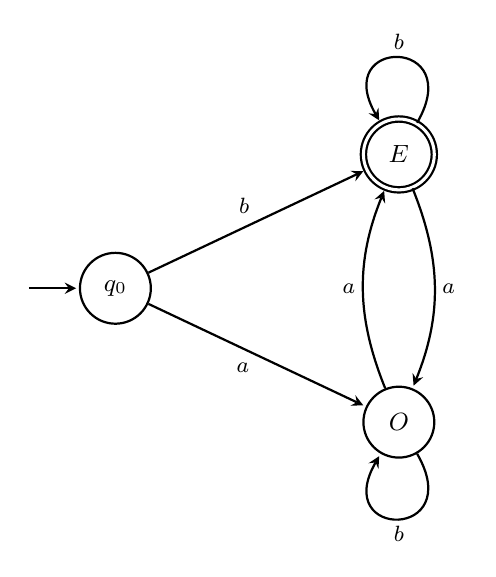
\begin{tikzpicture}
		\node[sta] (q0) at (0,0) {$q_0$};
		\node[acc] (E) at (3.6,1.7) {$E$};
		\node[sta] (O) at (3.6,-1.7) {$O$};
		\initarr{q0}{(-1.1,0)}
		\draw[tra] (q0) -- node[tlab, above left] {$b$} (E);
		\draw[tra] (q0) -- node[tlab, below left] {$a$} (O);
		\draw[tra] (E) to[bend left=22] node[tlab, right] {$a$} (O);
		\draw[tra] (O) to[bend left=22] node[tlab, left] {$a$} (E);
		\draw[tra] (E) to[out=60, in=120, looseness=7] node[tlab, above] {$b$} (E);
		\draw[tra] (O) to[out=-60, in=-120, looseness=7] node[tlab, below] {$b$} (O);
	\end{tikzpicture}
	\end{center}
	The states $E$ and $O$ record the parity of the number of $a$'s read so far, and $q_0$ is a copy of $E$ which exists only to keep $\eps$ out of the language. Thus $b$ is accepted ($q_0 \to E$), $aa$ is accepted ($q_0 \to O \to E$), and $a$ is rejected ($q_0 \to O$), as is $\eps$.
\end{example}

The last example is slightly unsatisfying: the states $q_0$ and $E$ do the same job. We will make this observation precise in Section~\ref{sec:minimisation}, where we show that every automaton has a canonical smallest equivalent form. To do that we need a notion of map between automata.

\begin{definition}[Homomorphism]
	Let $D = (\Sigma, Q, \delta, q_0, F)$ and $D' = (\Sigma, Q', \delta', q_0', F')$. A function $f \colon Q \to Q'$ is a \vocab{homomorphism} if
	\begin{enumerate}[label=(\roman*)]
		\item $\delta'(f(q), a) = f(\delta(q,a))$ for all $q \in Q$, $a \in \Sigma$;
		\item $f(q_0) = q_0'$;
		\item $q \in F$ if and only if $f(q) \in F'$.
	\end{enumerate}
	A bijective homomorphism is an \vocab{isomorphism}; its inverse is then a homomorphism too.
\end{definition}

Condition (i) says that $f$ commutes with a single step, and a trivial induction upgrades this to $\hat\delta'(f(q), w) = f(\hat\delta(q,w))$ for all words $w$.

\begin{proposition}\label{prop:homlanguage}
	If there is a homomorphism $f \colon D \to D'$ then $\lang(D) = \lang(D')$.
\end{proposition}

\begin{proof}
	For any word $w$ we have
	$$\hat\delta(q_0, w) \in F \iff f(\hat\delta(q_0,w)) \in F' \iff \hat\delta'(q_0', w) \in F'$$
	using (iii), then (i) and (ii). \end{proof}

So a homomorphism, even a very non-injective and non-surjective one, preserves the language. This tells us what failures of bijectivity mean. If $f$ is not surjective, the missing states of $D'$ are not reachable from $q_0'$. If $f$ is not injective, say $f(p) = f(q)$ with $p \neq q$, then for every word $w$
$$f(\hat\delta(p,w)) = \hat\delta'(f(p),w) = \hat\delta'(f(q),w) = f(\hat\delta(q,w)),$$
so $\hat\delta(p,w) \in F$ if and only if $\hat\delta(q,w) \in F$: the states $p$ and $q$ cannot be told apart by any word. Both phenomena are forms of redundancy, and eliminating them is exactly what minimisation does.

\subsection{From Automata to Grammars}

\begin{theorem}\label{thm:dfatogrammar}
	If $D$ is a deterministic automaton then $\lang(D)$ is regular.
\end{theorem}

\begin{proof}
	Let $D = (\Sigma, Q, \delta, q_0, F)$ and define a grammar $G = (\Sigma, Q, P, q_0)$ with variable set $Q$ and
	$$P = \{p \to aq \mid \delta(p,a) = q\} \cup \{p \to a \mid \delta(p,a) \in F\}.$$
	Every rule is regular. Now let $w = a_0a_1\cdots a_n$ be a nonempty word, and let $q_0, q_1, \dots, q_{n+1}$ be the state sequence of $D$ on $w$. Then
	\begin{align*}
		w \in \lang(D) &\iff q_{n+1} \in F \\
		&\iff q_i \to a_iq_{i+1} \in P \text{ for } i < n, \text{ and } q_n \to a_n \in P \\
		&\iff q_0 \Rightarrow_G a_0q_1 \Rightarrow_G \cdots \Rightarrow_G a_0\cdots a_{n-1}q_n \Rightarrow_G w,
	\end{align*}
	where the middle equivalence holds because the state sequence is uniquely determined by $w$. By Lemma~\ref{lem:regularlength} every derivation of $w$ in $G$ has this shape, so the last line holds if and only if $w \in \lang(G)$. Finally $\eps$ lies in neither language.
\end{proof}

We would like the converse. The obvious attempt -- take $Q = V$ and read off $\delta$ from the rules -- fails immediately, because a regular grammar may contain both $A \to aB$ and $A \to aB'$, and then there is no single value for $\delta(A,a)$. The standard remedy is to allow the machine to be in a \emph{set} of states at once.

\subsection{Nondeterministic Automata and the Subset Construction}

\begin{definition}[Nondeterministic automaton]
	A \vocab{nondeterministic automaton} is a tuple $N = (\Sigma, Q, \delta, q_0, F)$ exactly as before, except that
	$$\delta \colon Q \times \Sigma \to \power(Q).$$
\end{definition}

We read $\delta(q,a)$ as the set of states the machine \emph{may} move to on reading $a$ in state $q$; if $\delta(q,a) = \varnothing$ then the computation gets stuck. The graphical convention is unchanged, except that a node may now have several, or no, outgoing arrows for a given letter.

\begin{definition}
	For a nondeterministic automaton define $\hat\delta \colon Q \times \WW \to \power(Q)$ by
	$$\hat\delta(q, \eps) = \{q\}, \qquad \hat\delta(q, wa) = \bigcup_{p \in \hat\delta(q,w)} \delta(p,a),$$
	and set
	$$\lang(N) = \{w \in \WW \mid \hat\delta(q_0, w) \cap F \neq \varnothing\}.$$
\end{definition}

So $N$ accepts $w$ if \emph{some} run on $w$ ends in an accept state. A deterministic automaton is the special case in which every $\delta(q,a)$ is a singleton, and the two definitions of $\hat\delta$ then agree.

\begin{example}\label{ex:nfaendab}
	Let $\Sigma = \{a,b\}$ and consider the nondeterministic automaton $N$ with states $s$ (start), $t$ and $u$ (accept), and
	$$\delta(s,a) = \{s,t\}, \quad \delta(s,b) = \{s\}, \quad \delta(t,b) = \{u\},$$
	all other values being $\varnothing$.
	\begin{center}
	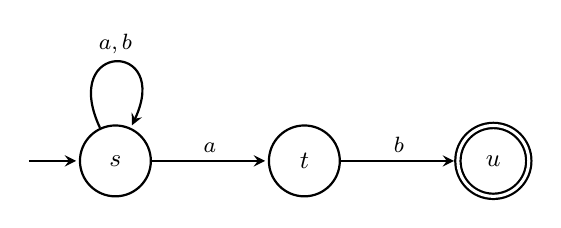
\begin{tikzpicture}
		\node[sta] (s) at (0,0) {$s$};
		\node[sta] (t) at (2.4,0) {$t$};
		\node[acc] (u) at (4.8,0) {$u$};
		\initarr{s}{(-1.1,0)}
		\draw[tra] (s) -- node[tlab, above] {$a$} (t);
		\draw[tra] (t) -- node[tlab, above] {$b$} (u);
		\draw[tra] (s) to[out=115, in=65, looseness=8] node[tlab, above] {$a,b$} (s);
	\end{tikzpicture}
	\end{center}
	The machine guesses when it has reached the penultimate letter. It accepts exactly the words ending in $ab$: on input $aab$ we get $\hat\delta(s,a) = \{s,t\}$, then $\hat\delta(s,aa) = \{s,t\}$, then $\hat\delta(s,aab) = \{s\} \cup \{u\} = \{s,u\}$, which meets $F$; whereas on input $aba$ we get $\{s,t\}$, then $\{s,u\}$, then $\{s,t\}$, which does not.
\end{example}

The nondeterminism is only apparent, and this is the fundamental theorem about finite automata.

\begin{theorem}[Subset construction]\label{thm:subset}
	Let $N$ be a nondeterministic automaton. Then there is a deterministic automaton $D$ with $\lang(N) = \lang(D)$.
\end{theorem}

\begin{proof}
	Let $N = (\Sigma, Q, \delta, q_0, F)$ and define
	$$D = (\Sigma,\; \power(Q),\; \Delta,\; \{q_0\},\; \mathcal{F}), \qquad \Delta(X, a) = \bigcup_{q \in X} \delta(q, a),$$
	$$\mathcal{F} = \{X \subseteq Q \mid X \cap F \neq \varnothing\}.$$
	(If $\{q_0\} \in \mathcal{F}$, that is if $q_0 \in F$, then $F$ was not a legal accept set for $N$ in the first place; so the convention $\mathcal{F} \subseteq \power(Q) \setminus \{\{q_0\}\}$ holds automatically.)

	Fix a word $w = a_0\cdots a_{n-1}$. The state sequence of $D$ on $w$ is $X_0 = \{q_0\}$ and $X_{i+1} = \bigcup_{q \in X_i}\delta(q, a_i)$; the sequence of state-sets of $N$ is $Y_0 = \{q_0\}$ and $Y_{i+1} = \bigcup_{q \in Y_i}\delta(q,a_i)$. These recursions are identical, so $X_i = Y_i$ for all $i$, whence
	$$w \in \lang(D) \iff X_n \cap F \neq \varnothing \iff \hat\delta(q_0,w) \cap F \neq \varnothing \iff w \in \lang(N). \qedhere$$
\end{proof}

\begin{remark}
	The construction turns an $n$-state machine into one with $2^n$ states, and this exponential blow-up cannot in general be avoided. In practice one only ever builds the subsets \emph{reachable} from $\{q_0\}$, which is often far fewer.
\end{remark}

\begin{example}\label{ex:subsetworked}
	Let us carry out the subset construction on the automaton $N$ of Example~\ref{ex:nfaendab}. Starting from $\{s\}$ and closing off under $\Delta$:
	$$\Delta(\{s\},a) = \{s,t\}, \quad \Delta(\{s\},b) = \{s\}, \quad \Delta(\{s,t\},a) = \{s,t\}, \quad \Delta(\{s,t\},b) = \{s,u\},$$
	$$\Delta(\{s,u\},a) = \{s,t\}, \quad \Delta(\{s,u\},b) = \{s\}.$$
	Only three of the eight subsets are reachable, and only $\{s,u\}$ meets $F = \{u\}$. Writing $X = \{s\}$, $Y = \{s,t\}$, $Z = \{s,u\}$ we obtain the deterministic automaton $D$ drawn on the right below, beside the original $N$.
	\begin{center}
	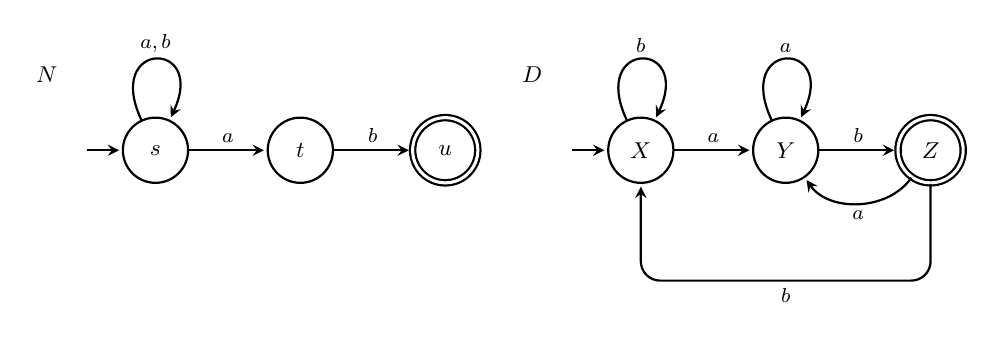
\begin{tikzpicture}[scale=0.92, transform shape]
		% NFA
		\node[font=\small] at (-1.5,1.05) {$N$};
		\node[sta] (s) at (0,0) {$s$};
		\node[sta] (t) at (2.0,0) {$t$};
		\node[acc] (u) at (4.0,0) {$u$};
		\initarr{s}{(-0.95,0)}
		\draw[tra] (s) -- node[tlab, above] {$a$} (t);
		\draw[tra] (t) -- node[tlab, above] {$b$} (u);
		\draw[tra] (s) to[out=115, in=65, looseness=8] node[tlab, above] {$a,b$} (s);
		% DFA
		\begin{scope}[xshift=6.7cm]
		\node[font=\small] at (-1.5,1.05) {$D$};
		\node[sta] (X) at (0,0) {$X$};
		\node[sta] (Y) at (2.0,0) {$Y$};
		\node[acc] (Z) at (4.0,0) {$Z$};
		\initarr{X}{(-0.95,0)}
		\draw[tra] (X) -- node[tlab, above] {$a$} (Y);
		\draw[tra] (Y) -- node[tlab, above] {$b$} (Z);
		\draw[tra] (X) to[out=115, in=65, looseness=8] node[tlab, above] {$b$} (X);
		\draw[tra] (Y) to[out=115, in=65, looseness=8] node[tlab, above] {$a$} (Y);
		\draw[tra] (Z) to[out=-125, in=-55] node[tlab, below] {$a$} (Y);
		\draw[tra, rounded corners=7pt] (Z) -- (4.0,-1.8) -- node[tlab, below] {$b$} (0,-1.8) -- (X);
		\end{scope}
	\end{tikzpicture}
	\end{center}
	Tracing $abab$ through $D$: $X \to Y \to Z \to Y \to Z$, ending in the accept state, and indeed $abab$ ends in $ab$. Tracing $abb$: $X \to Y \to Z \to X$, rejected, and indeed $abb$ does not end in $ab$.
\end{example}

\begin{theorem}\label{thm:grammartonfa}
	If $G$ is a regular grammar then there is a nondeterministic automaton $N$ with $\lang(G) = \lang(N)$.
\end{theorem}

\begin{proof}
	Let $G = (\Sigma, V, P, S)$ and let $H$ be a fresh symbol, the \vocab{halt state}. Put $Q = V \cup \{H\}$ and define $N = (\Sigma, Q, \delta, S, \{H\})$ where, for $A \in V$,
	$$\delta(A, a) = \begin{cases} \{B \mid A \to aB \in P\} & \text{if } A \to a \notin P, \\ \{B \mid A \to aB \in P\} \cup \{H\} & \text{if } A \to a \in P,\end{cases}$$
	and $\delta(H,a) = \varnothing$. Note $H \neq S$, so the convention $F \subseteq Q \setminus \{q_0\}$ holds.

	Let $w = a_0\cdots a_n$ be a nonempty word. By Lemma~\ref{lem:regularlength}, $w \in \lang(G)$ if and only if there are variables $S = A_0, A_1, \dots, A_n$ with $A_i \to a_iA_{i+1} \in P$ for $i < n$ and $A_n \to a_n \in P$. By the definition of $\delta$, this holds if and only if there are states with $A_{i+1} \in \delta(A_i, a_i)$ for $i < n$ and $H \in \delta(A_n, a_n)$, which holds if and only if $H \in \hat\delta(S, w)$, i.e.\ $w \in \lang(N)$. Neither language contains $\eps$.
\end{proof}

Assembling Theorems~\ref{thm:dfatogrammar},~\ref{thm:subset} and~\ref{thm:grammartonfa}, we have the following, which is the first genuinely satisfying theorem of the course.

\begin{corollary}\label{cor:threeequiv}
	For a language $L$, the following are equivalent:
	\begin{enumerate}[label=(\roman*)]
		\item $L$ is regular, i.e.\ $L = \lang(G)$ for a regular grammar $G$;
		\item $L = \lang(N)$ for a nondeterministic automaton $N$;
		\item $L = \lang(D)$ for a deterministic automaton $D$.
	\end{enumerate}
	Moreover, each translation is effective: given one of the three objects we can compute the other two.
\end{corollary}

\subsection{The Pumping Lemma for Regular Languages}

We now have three ways to show a language \emph{is} regular. To show that one is not, the standard tool is the following. It expresses in combinatorial terms the fact that a machine with finitely many states must, on a long enough word, revisit a state, and can then be made to go round the resulting loop as often as we please.

\begin{definition}[Regular pumping lemma]
	A language $L$ \vocab{satisfies the regular pumping lemma with pumping number $n$} if every $w \in L$ with $\abs{w} \geq n$ can be written as $w = xyz$ with
	$$\abs{y} > 0, \qquad \abs{xy} \leq n, \qquad xy^kz \in L \text{ for all } k \in \N.$$
	We call $y$ a \vocab{pump} for $w$.
\end{definition}

\begin{theorem}[Pumping lemma]\label{thm:regpumping}
	Every regular language satisfies the regular pumping lemma, with pumping number the number of states of any deterministic automaton accepting it.
\end{theorem}

\begin{proof}
	Let $L = \lang(D)$ with $D = (\Sigma, Q, \delta, q_0, F)$, and put $n = \abs{Q}$. Let $w \in L$ with $\abs{w} \geq n$, say $w = a_0a_1\cdots a_{n-1}v$.

	Let $q_0, q_1, \dots, q_n$ be the states visited while reading $a_0 \cdots a_{n-1}$. This is a list of $n+1$ states drawn from a set of size $n$, so by pigeonhole there are $i < j \leq n$ with $q_i = q_j$. Put
	$$x = a_0\cdots a_{i-1}, \qquad y = a_i \cdots a_{j-1}, \qquad z = a_j \cdots a_{n-1}v,$$
	so that $xyz = w$, $\abs{y} = j - i > 0$ and $\abs{xy} = j \leq n$.

	Now $\hat\delta(q_0, x) = q_i$ and $\hat\delta(q_i, y) = q_j = q_i$, so by induction on $k$ we get $\hat\delta(q_0, xy^k) = q_i$ for every $k \in \N$. Finally $\hat\delta(q_i, z) = \hat\delta(q_j, z) = \hat\delta(q_0,w) \in F$, so $\hat\delta(q_0, xy^kz) \in F$ and $xy^kz \in L$.
\end{proof}

The picture behind the proof is worth drawing: the accepting path through the machine, of length at least $n$, must contain a loop within its first $n$ steps, and the loop can be traversed any number of times.

\begin{center}
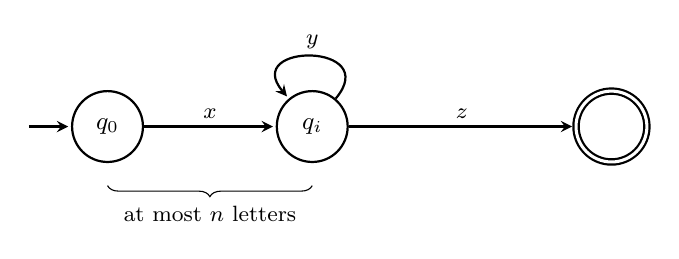
\begin{tikzpicture}
	\node[sta] (a) at (0,0) {$q_0$};
	\node[sta] (b) at (2.6,0) {$q_i$};
	\node[acc] (c) at (6.4,0) {};
	\initarr{a}{(-1.0,0)}
	\draw[tra] (a) -- node[tlab, above] {$x$} (b);
	\draw[tra] (b) -- node[tlab, above] {$z$} (c);
	\draw[tra] (b) to[out=50, in=130, looseness=4] node[tlab, above] {$y$} (b);
	\draw[decorate, decoration={brace, amplitude=4pt, mirror}] (0,-0.75) -- node[below=4pt, font=\footnotesize] {at most $n$ letters} (2.6,-0.75);
\end{tikzpicture}
\end{center}

\begin{example}\label{ex:0k1knotregular}
	The language $L = \{0^k1^k \mid k > 0\}$ is not regular.

	Suppose it were, with pumping number $N$. The word $w = 0^N1^N$ lies in $L$ and has length $2N \geq N$, so it can be written $w = xyz$ with $\abs{xy} \leq N$ and $\abs{y} = \ell > 0$. Since $\abs{xy} \leq N$, the pump $y$ lies within the first $N$ letters of $w$, all of which are $0$s; so $y = 0^\ell$. Pumping down with $k = 0$ gives $xz = 0^{N - \ell}1^N \in L$, which is false since $\ell > 0$. So $L$ is not regular.
\end{example}

We will see in Section~\ref{sec:cfl} that $L = \{0^k1^k\}$ \emph{is} context-free, so this example already shows that the inclusion of type 3 in type 2 is strict.

\begin{example}\label{ex:needstates}
	Fix $n \geq 2$ and let $L = \{0^n w \mid w \in \WW\}$, the words beginning with $n$ zeroes. This is regular: take $V = \{S, X_0, \dots, X_{n-1}\}$ and
	\begin{align*}
		P = \{S \to 0X_0\} &\cup \{X_i \to 0X_{i+1} \mid i \leq n - 3\} \cup \{X_{n-2} \to 0X_{n-1},\; X_{n-2} \to 0\} \\
		&\cup \{X_{n-1} \to 0,\; X_{n-1} \to 1,\; X_{n-1} \to 0X_{n-1},\; X_{n-1} \to 1X_{n-1}\}.
	\end{align*}
	But no deterministic automaton with at most $n$ states accepts $L$. Indeed, such an automaton would give $L$ pumping number $n$ by Theorem~\ref{thm:regpumping}, and then the word $0^n \in L$ of length $n$ could be pumped down to a word with fewer than $n$ zeroes, which is not in $L$.
\end{example}

It is essential to remember that the pumping lemma is a necessary but \emph{not} a sufficient condition for regularity. The next example makes this vivid.

\begin{example}\label{ex:pumpingnotsufficient}
	Let $\Sigma = \{0,1\}$. For a word $w$ containing at least one $0$, define the \vocab{tail} of $w$ to be the number of $1$s following the last $0$. Given $X \subseteq \N$, let
	$$L_X = \{w \in \WW^+ \mid w \text{ contains no } 0\} \cup \{w \mid w \text{ has a tail lying in } X\}.$$
	If $X \neq Y$ then $L_X \neq L_Y$: taking $m$ in the symmetric difference, the word $01^m$ distinguishes them. So $X \mapsto L_X$ is injective, and since $\power(\N)$ is uncountable while there are only countably many regular languages, some $L_X$ is not regular.

	Nevertheless \emph{every} $L_X$ satisfies the pumping lemma with pumping number $2$. Let $w \in L_X$ with $\abs{w} \geq 2$.
	\begin{itemize}
		\item If $w = 0z$, take $x = \eps$, $y = 0$. Pumping up prepends more $0$s, which changes neither the presence of a $0$ nor the tail. Pumping down gives $z$: either $z$ still contains a $0$, in which case the tail is unchanged, or it does not, in which case $z \in 1^\star$ and again lies in $L_X$ (note $z \neq \eps$ as $\abs{w} \geq 2$).
		\item If $w = 1z$, take $x = \eps$, $y = 1$. If $z$ contains no $0$ then neither does $1^kz$, so all pumps lie in $L_X$. If $z$ contains a $0$ then the tail of $1^kz$ equals the tail of $z$ for every $k$, so again all pumps lie in $L_X$.
	\end{itemize}
	Hence there are uncountably many languages satisfying the regular pumping lemma, and in particular the pumping lemma does not characterise the regular languages.
\end{example}

\subsection{Closure Properties}

We have already proved closure under union (Theorem~\ref{thm:closureunionconcat} together with the automaton translation, or directly) and concatenation (Lemma~\ref{lem:regconcat}). Automata make the Boolean operations easy.

\begin{proposition}\label{prop:regcomplement}
	The regular languages are closed under complement (relative to $\WW^+$), intersection and difference.
\end{proposition}

\begin{proof}
	Let $L = \lang(D)$ with $D = (\Sigma, Q, \delta, q_0, F)$. We may assume that no transition enters the start state, that is, that $\delta(q,a) \neq q_0$ for all $q$ and $a$. Indeed, if this fails, adjoin a fresh state $q_0'$, put $\delta(q_0',a) = \delta(q_0,a)$ for every letter $a$, and take $q_0'$ as the new start state, demoting $q_0$ to an ordinary state (which is not accepting, since $q_0 \notin F$). No transition enters $q_0'$, and $\hat\delta(q_0',w) = \hat\delta(q_0,w)$ for every nonempty $w$, so the language is unchanged. We rename $q_0'$ back to $q_0$.

	Now set $D' = (\Sigma, Q, \delta, q_0, Q \setminus (F \cup \{q_0\}))$. For a nonempty word $w$ we have $\hat\delta(q_0,w) \neq q_0$, so $\hat\delta(q_0,w) \in Q \setminus (F \cup \{q_0\})$ if and only if $\hat\delta(q_0,w) \notin F$. Hence $\lang(D') = \WW^+ \setminus L$.

	Intersection and difference now follow from De Morgan, since $L \cap M = \WW^+ \setminus ((\WW^+ \setminus L) \cup (\WW^+ \setminus M))$ and $L \setminus M = L \cap (\WW^+ \setminus M)$.
\end{proof}

There is a more direct construction for intersection and union which is worth knowing, because it is the one that fails for the higher classes.

\begin{definition}[Product automaton]
	Given $D = (\Sigma, Q, \delta, q_0, F)$ and $D' = (\Sigma, Q', \delta', q_0', F')$, the \vocab{product automaton} is
	$$D \times D' = (\Sigma,\; Q \times Q',\; \delta \times \delta',\; (q_0,q_0'),\; F''), \qquad (\delta\times\delta')((q,q'),a) = (\delta(q,a), \delta'(q',a)),$$
	where $F''$ is either $\{(q,q') \mid q \in F \text{ and } q' \in F'\}$ or $\{(q,q') \mid q \in F \text{ or } q' \in F'\}$.
\end{definition}

An immediate induction gives $(\widehat{\delta\times\delta'})((q_0,q_0'),w) = (\hat\delta(q_0,w), \hat\delta'(q_0',w))$, so the first choice of $F''$ yields $\lang(D)\cap\lang(D')$ and the second yields $\lang(D)\cup\lang(D')$. In words: the product machine runs both automata side by side on the same input, which it can afford to do because each has only finitely many states. We will see in Section~\ref{sec:cfl} that no such construction can exist for context-free languages.

\subsection{Regular Expressions and Kleene's Theorem}

There is a fourth description of the regular languages, and it is the one familiar from programming.

\begin{definition}[Kleene star]
	For a language $L$, the \vocab{Kleene star} of $L$ is
	$$L^\star = \{w_1w_2\cdots w_k \mid k \in \N,\; w_i \in L\},$$
	the set of all concatenations of finitely many words of $L$; in particular $\eps \in L^\star$, taking $k = 0$. The \vocab{Kleene plus} is $L^+ = \{w_1\cdots w_k \mid k \geq 1,\; w_i \in L\}$, so that $L^\star = L^+ \cup \{\eps\}$.
\end{definition}

\begin{definition}[Regular expression]
	The \vocab{regular expressions} over $\Sigma$ are defined inductively:
	\begin{enumerate}[label=(\roman*)]
		\item $\varnothing$ is a regular expression;
		\item $\eps$ is a regular expression;
		\item $a$ is a regular expression for each $a \in \Sigma$;
		\item if $R,S$ are regular expressions then so is $(R+S)$;
		\item if $R,S$ are regular expressions then so is $(RS)$;
		\item if $R$ is a regular expression then so are $R^\star$ and $R^+$,
	\end{enumerate}
	and nothing else is. To each regular expression $E$ we assign a language $\lang(E)$ by the matching recursion:
	$$\lang(\varnothing) = \varnothing, \quad \lang(\eps) = \{\eps\}, \quad \lang(a) = \{a\},$$
	$$\lang(R+S) = \lang(R)\cup\lang(S), \quad \lang(RS) = \lang(R)\lang(S),$$
	$$\lang(R^\star) = \lang(R)^\star, \quad \lang(R^+) = \lang(R)^+.$$
\end{definition}

We drop parentheses when no ambiguity results, giving concatenation a higher binding power than $+$, so that $RS + T$ means $((RS)+T)$.

The only irritation is the empty word, which regular expressions can produce and regular grammars cannot. We deal with it by a definition.

\begin{definition}
	A language $L$ is \vocab{essentially regular} if $L$ or $L \setminus \{\eps\}$ is regular; equivalently, if there is a regular $L'$ with $L = L'$ or $L = L' \cup \{\eps\}$.
\end{definition}

\begin{theorem}\label{thm:regextoreg}
	If $E$ is a regular expression then $\lang(E)$ is essentially regular.
\end{theorem}

\begin{proof}
	We induct on the structure of $E$. The base cases are clear: $\varnothing$ and $\{a\}$ are regular (take $P = \varnothing$ and $P = \{S \to a\}$ respectively) and $\{\eps\} = \varnothing \cup \{\eps\}$ is essentially regular.

	For the induction step it is enough to show that essentially regular languages are closed under union, concatenation and Kleene plus, since $\lang(E^\star) = \lang(E + E^+)$.

	Union and concatenation of regular languages are regular by Theorem~\ref{thm:closureunionconcat} and Lemma~\ref{lem:regconcat}, and the extension to essentially regular languages is a short case analysis: for instance $(L\cup\{\eps\})(M\cup\{\eps\}) = LM \cup L \cup M \cup \{\eps\}$, and $LM \cup L \cup M$ is regular.

	So let $G = (\Sigma, V, P, S)$ be regular; we must show $\lang(G)^+$ is regular. We may assume $G$ is $\eps$-adequate, so $S$ never occurs on the right of a rule. Let
	$$P^+ = P \cup \{A \to aS \mid A \to a \in P\}, \qquad G^+ = (\Sigma, V, P^+, S).$$
	This is regular; we claim $\lang(G^+) = \lang(G)^+$.

	($\supseteq$) Let $w = w_0w_1\cdots w_n$ with each $w_i \in \lang(G)$. Induct on $n$. For $n = 0$ any $G$-derivation is a $G^+$-derivation. For $n > 0$, by induction $S \Rightarrow_{G^+}^\star w_0\cdots w_{n-1}$; this derivation ends with a terminal rule $A \to a$, and replacing that final step by $A \to aS$ gives $S \Rightarrow_{G^+}^\star w_0\cdots w_{n-1}S$. Appending a $G$-derivation of $w_n$ gives $w$.

	($\subseteq$) Let $S \Rightarrow_{G^+}^\star w$ and let $n \geq 1$ be the number of strings in the derivation in which $S$ occurs (the first one always does). Induct on $n$. If $n = 1$ then $S$ occurs only at the start, so no added rule was used and $S \Rightarrow_G^\star w$, giving $w \in \lang(G) \subseteq \lang(G)^+$. If $n > 1$, write the derivation as $S \Rightarrow_{G^+}^\star vS \Rightarrow_{G^+}^\star w$ where $vS$ is the \emph{last} string containing $S$. The step producing $vS$ used an added rule $A \to aS$; replacing it by $A \to a$ gives a derivation $S \Rightarrow_{G^+}^\star v$ with $n - 1$ occurrences of $S$, so $v \in \lang(G)^+$ by induction. From $vS$ onward $S$ never reappears, so no added rule fires, and $w = vw'$ with $S \Rightarrow_G^\star w'$, i.e.\ $w' \in \lang(G)$. Hence $w \in \lang(G)^+$.
\end{proof}

The converse is Kleene's theorem proper, and it is usually proved by an algorithm which eliminates the states of an automaton one at a time. We give the closely related dynamic-programming version.

\begin{theorem}[Kleene]\label{thm:kleene}
	Let $D$ be a deterministic automaton. Then there is a regular expression $E$ with $\lang(E) = \lang(D)$. Consequently a language is essentially regular if and only if it is $\lang(E)$ for some regular expression $E$.
\end{theorem}

\begin{proof}
	Write $Q = \{q_0, q_1, \dots, q_{m-1}\}$. For $i, j < m$ and $0 \leq k \leq m$, let
	$$R^k_{i,j} = \{w \in \WW \mid \hat\delta(q_i, w) = q_j \text{, all states strictly inside}$$
	$$\text{the run lying in } \{q_0, \dots, q_{k-1}\}\},$$
	where `strictly inside' means excluding the first and last states of the run. We show by induction on $k$ that each $R^k_{i,j}$ is $\lang(E)$ for a regular expression $E^k_{i,j}$.

	For $k = 0$ no intermediate states are allowed, so $R^0_{i,j}$ consists of $\eps$ (if $i = j$) together with the letters $a$ with $\delta(q_i,a) = q_j$. This is a finite set of words of length at most $1$, hence is $\lang(E)$ for a finite sum of the base expressions.

	For the induction step, a run from $q_i$ to $q_j$ through $\{q_0,\dots,q_k\}$ either avoids $q_k$ altogether, or visits $q_k$; in the latter case, splitting at the first and last visits to $q_k$ decomposes the word as a run $q_i \to q_k$ avoiding $q_k$ internally, then finitely many runs $q_k \to q_k$ avoiding $q_k$ internally, then a run $q_k \to q_j$ avoiding $q_k$ internally. Hence
	$$R^{k+1}_{i,j} = R^k_{i,j} \cup R^k_{i,k}\left(R^k_{k,k}\right)^\star R^k_{k,j},$$
	and we may take $E^{k+1}_{i,j} = E^k_{i,j} + E^k_{i,k}(E^k_{k,k})^\star E^k_{k,j}$.

	Finally $\lang(D) = \bigcup_{q_j \in F} R^m_{0,j}$, so we take $E = \sum_{q_j \in F} E^m_{0,j}$. Since $q_0 \notin F$, the word $\eps$ does not lie in this language, so the resulting expression describes $\lang(D)$ exactly.

	For the last sentence, combine this with Theorem~\ref{thm:regextoreg}: if $L$ is essentially regular then $L$ is $\lang(E)$ or $\lang(E + \eps)$ for a suitable $E$.
\end{proof}

\begin{example}
	The automaton of Example~\ref{ex:atleastonezero} accepts the words containing at least one $0$, and indeed
	$$\lang(D) = \lang\big(1^\star 0 (0+1)^\star\big).$$
	The automaton of Example~\ref{ex:subsetworked} accepts $\lang((a+b)^\star ab)$.
\end{example}

\subsection{Minimisation}\label{sec:minimisation}

We saw in Example~\ref{ex:evenas} an automaton with two states doing the same job. We now make this precise and show that every regular language has a canonical smallest automaton.

\begin{definition}
	A state $q$ is \vocab{accessible} if $q = \hat\delta(q_0, w)$ for some $w \in \WW$, and \vocab{inaccessible} otherwise.

	States $q, q'$ are \vocab{distinguished by $w$} if exactly one of $\hat\delta(q,w)$, $\hat\delta(q',w)$ lies in $F$. They are \vocab{distinguishable} if some word distinguishes them, and \vocab{indistinguishable} otherwise; we write $q \sim q'$ in the latter case.

	$D$ is \vocab{irreducible} if every state is accessible and every pair of distinct states is distinguishable.
\end{definition}

Suppose $f \colon D \to D'$ is a homomorphism. If $p,q$ are distinguishable by $w$ then, since $f$ commutes with $\hat\delta$ and preserves acceptance, $f(p)$ and $f(q)$ are distinguished by $w$, so $f(p) \neq f(q)$. And if $q' \in Q'$ is accessible, say $q' = \hat\delta'(q_0',w)$, then $q' = f(\hat\delta(q_0,w))$ lies in the image of $f$. Hence:

\begin{proposition}\label{prop:irreduciblehom}
	Any homomorphism between irreducible automata is an isomorphism.
\end{proposition}

Clearly $\sim$ is an equivalence relation on $Q$; write $[q]$ for the class of $q$.

\begin{definition}[Quotient automaton]
	Define
	$$D/{\sim} \;=\; \big(\Sigma,\; Q/{\sim},\; [\delta],\; [q_0],\; [F]\big), \qquad [\delta]([q],a) = [\delta(q,a)], \qquad [F] = \{[q] \mid q \in F\}.$$
\end{definition}

Two checks are needed. First, being accepting is a class property: if $q \sim q'$ then $\eps$ does not distinguish them, so $q \in F \iff q' \in F$; in particular $[F]$ really is a set of classes, and $[q_0] \notin [F]$ since $q_0 \notin F$. Second, $[\delta]$ is well defined: if $q \sim q'$ but $\delta(q,a) \not\sim \delta(q',a)$, witnessed by a word $w$, then $aw$ would distinguish $q$ from $q'$.

\begin{lemma}\label{lem:quotient}
	The quotient map $q \mapsto [q]$ is a surjective homomorphism, so $\lang(D) = \lang(D/{\sim})$. Moreover distinct states of $D/{\sim}$ are distinguishable, and if every state of $D$ is accessible then so is every state of $D/{\sim}$.
\end{lemma}

\begin{proof}
	That the quotient map is a homomorphism is exactly the two checks above; it is surjective by construction, so accessibility is inherited and Proposition~\ref{prop:homlanguage} gives the languages agree.

	An easy induction gives $[\hat\delta]([q],w) = [\hat\delta(q,w)]$. Now suppose $[q] \neq [q']$, so $q \not\sim q'$; take $w$ distinguishing them, say $\hat\delta(q,w) \in F$ and $\hat\delta(q',w) \notin F$. Then $[\hat\delta]([q],w) = [\hat\delta(q,w)] \in [F]$ while $[\hat\delta]([q'],w) \notin [F]$, so $w$ distinguishes $[q]$ from $[q']$.
\end{proof}

\begin{theorem}\label{thm:irreducibleexists}
	For every deterministic automaton $D$ there is an irreducible deterministic automaton $I$ with $\lang(D) = \lang(I)$ and at most as many states.
\end{theorem}

\begin{proof}
	Let $A \subseteq Q$ be the set of accessible states; note $q_0 \in A$ and $\delta$ restricts to $A$. Put $D^\star = (\Sigma, A, \delta\restriction_{A\times\Sigma}, q_0, F \cap A)$. The inclusion $A \hookrightarrow Q$ is a homomorphism, so $\lang(D^\star) = \lang(D)$, and every state of $D^\star$ is accessible. Now take $I = D^\star/{\sim}$ and apply Lemma~\ref{lem:quotient}.
\end{proof}

\begin{theorem}\label{thm:irreducibleunique}
	If $I$ and $I'$ are irreducible with $\lang(I) = \lang(I')$, then $I \cong I'$.
\end{theorem}

\begin{proof}
	By Proposition~\ref{prop:irreduciblehom} it suffices to construct a homomorphism $I \to I'$. Write $I = (\Sigma, Q, \delta, q_0, F)$ and $I' = (\Sigma, Q', \delta', q_0', F')$ with $Q \cap Q' = \varnothing$. Extend $\sim$ to $Q \cup Q'$ by declaring $q \sim q'$ (for $q \in Q$, $q' \in Q'$) when for all $w$, $\hat\delta(q,w) \in F \iff \hat\delta'(q',w) \in F'$; this is again an equivalence relation. Since the languages agree, $q_0 \sim q_0'$.

	\emph{Every $q \in Q$ is $\sim$-equivalent to some $q' \in Q'$.} Let $\mathrm{sp}(q)$ be the length of a shortest word $w$ with $\hat\delta(q_0,w) = q$, which exists by accessibility. Induct on $\mathrm{sp}(q)$. If $\mathrm{sp}(q) = 0$ then $q = q_0 \sim q_0'$. If $\mathrm{sp}(q) = k+1$, choose $p$ and $a$ with $\delta(p,a) = q$ and $\mathrm{sp}(p) = k$; by induction pick $p' \sim p$ and set $q' = \delta'(p',a)$. If $w$ is any word then $\hat\delta(q,w) = \hat\delta(p,aw)$ and $\hat\delta'(q',w) = \hat\delta'(p',aw)$, so $p \sim p'$ gives $q \sim q'$.

	\emph{The witness is unique.} If $q' \sim q \sim p'$ with $q',p' \in Q'$ then $q' \sim p'$ by transitivity, and irreducibility of $I'$ forces $q' = p'$.

	So there is a well-defined $f \colon Q \to Q'$ with $q \sim f(q)$. Then $f(q_0) = q_0'$; taking $w = \eps$ in the definition of $\sim$ gives $q \in F \iff f(q) \in F'$; and for any $a$, the computation above shows $\delta(q,a) \sim \delta'(f(q),a)$, so $f(\delta(q,a)) = \delta'(f(q),a)$ by uniqueness. Thus $f$ is a homomorphism.
\end{proof}

\begin{corollary}
	Every regular language is accepted by an irreducible automaton, unique up to isomorphism, and this automaton has fewer states than any other automaton accepting the language.
\end{corollary}

\begin{proof}
	Existence and uniqueness are Theorems~\ref{thm:irreducibleexists} and~\ref{thm:irreducibleunique}. If $D$ is any automaton for $L$, Theorem~\ref{thm:irreducibleexists} produces an irreducible $I$ with at most $\abs{Q}$ states, and $I$ is isomorphic to the canonical one.
\end{proof}

\begin{example}
	Return to Example~\ref{ex:atleastonezero}. Is that automaton irreducible? All three states are accessible. The state $q_1$ is distinguished from the others by $\eps$. But for any word $w$,
	$$\hat\delta(q_0, w) \in F \iff w \text{ contains a } 0 \iff \hat\delta(q_2, w) \in F,$$
	so $q_0 \sim q_2$ and the automaton is not irreducible. Quotienting merges them, and we obtain the two-state machine
	\begin{center}
	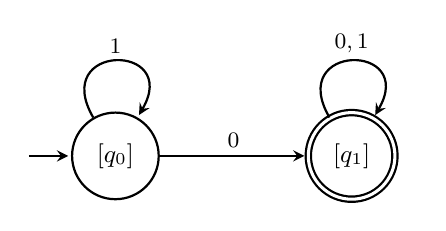
\begin{tikzpicture}[sta/.append style={minimum size=11mm}]
		\node[sta] (a) at (0,0) {$[q_0]$};
		\node[acc] (b) at (3,0) {$[q_1]$};
		\initarr{a}{(-1.1,0)}
		\draw[tra] (a) -- node[tlab, above] {$0$} (b);
		\draw[tra] (a) to[out=120, in=60, looseness=5] node[tlab, above] {$1$} (a);
		\draw[tra] (b) to[out=120, in=60, looseness=5] node[tlab, above] {$0,1$} (b);
	\end{tikzpicture}
	\end{center}
	which is irreducible. Notice that this still satisfies our convention that the start state is not accepting, as it must, since $\eps$ contains no $0$. Applying the same analysis to Example~\ref{ex:evenas} merges $q_0$ with $E$ and produces the expected two-state parity machine.
\end{example}

\subsection{The Myhill--Nerode Theorem}

Where do the states of the minimal automaton come from? The answer is that they are determined by the language alone, with no reference to any machine.

\begin{definition}[Nerode equivalence]
	Let $L \subseteq \WW$ be any language. For $u, v \in \WW$ write
	$$u \sim_L v \quad\text{if and only if}\quad \text{for all } w \in \WW, \; uw \in L \iff vw \in L.$$
	This is an equivalence relation on $\WW$; write $[u]_L$ for the class of $u$ and $\WW/{\sim_L}$ for the set of classes. It is a \vocab{right congruence}: if $u \sim_L v$ then $ua \sim_L va$ for every letter $a$.
\end{definition}

The relation $\sim_L$ says that $u$ and $v$ have the same \emph{future}: no continuation can tell them apart. If a machine is reading $L$ and has seen $u$, the only thing it can usefully remember is $[u]_L$.

\begin{center}
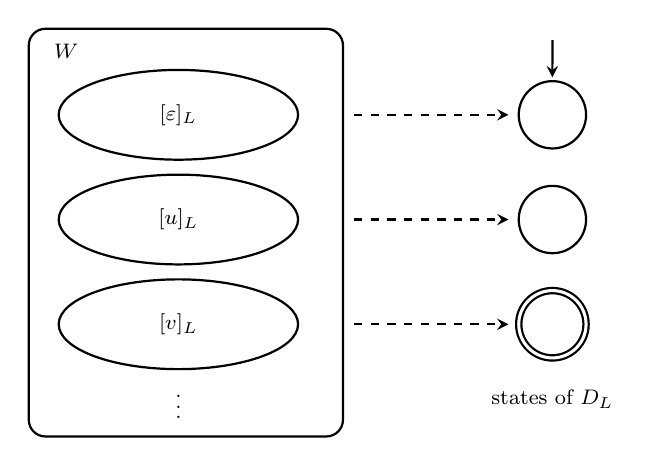
\begin{tikzpicture}[scale=0.95, transform shape]
	\draw[blob] (0,-2.9) rectangle (4.2,2.55);
	\node[font=\footnotesize] at (0.5,2.25) {$\WW$};
	\draw[thick] (2.0,1.4) ellipse (1.6 and 0.6);
	\draw[thick] (2.0,0.0) ellipse (1.6 and 0.6);
	\draw[thick] (2.0,-1.4) ellipse (1.6 and 0.6);
	\node[font=\footnotesize] at (2.0,1.4) {$[\eps]_L$};
	\node[font=\footnotesize] at (2.0,0.0) {$[u]_L$};
	\node[font=\footnotesize] at (2.0,-1.4) {$[v]_L$};
	\node[font=\footnotesize] at (2.0,-2.4) {$\vdots$};
	\node[sta] (se) at (7.0,1.4) {};
	\node[sta] (su) at (7.0,0.0) {};
	\node[acc] (sv) at (7.0,-1.4) {};
	\initarr{se}{(0,1.0)}
	\draw[tra, dashed] (4.35,1.4) -- (6.45,1.4);
	\draw[tra, dashed] (4.35,0.0) -- (6.45,0.0);
	\draw[tra, dashed] (4.35,-1.4) -- (6.45,-1.4);
	\node[font=\footnotesize] at (7.0,-2.4) {states of $D_L$};
\end{tikzpicture}
\end{center}

\begin{theorem}[Myhill--Nerode]\label{thm:myhillnerode}
	Let $L \subseteq \WW$ with $\eps \notin L$. Then $L$ is regular if and only if $\sim_L$ has finitely many equivalence classes. In that case the number of classes is the number of states of the minimal automaton for $L$.
\end{theorem}

\begin{proof}
	($\Rightarrow$) Let $L = \lang(D)$ for a deterministic $D$ with state set $Q$. If $\hat\delta(q_0,u) = \hat\delta(q_0,v)$ then for every $w$
	\begin{align*}
		uw \in L &\iff \hat\delta(q_0,uw) \in F \iff \hat\delta(\hat\delta(q_0,u),w) \in F \\
		&\iff \hat\delta(\hat\delta(q_0,v),w) \in F \iff vw \in L,
	\end{align*}
	so $u \sim_L v$. Hence $u \mapsto \hat\delta(q_0,u)$ induces a well-defined surjection from a subset of $Q$ onto $\WW/{\sim_L}$, and there are at most $\abs{Q}$ classes.

	($\Leftarrow$) Suppose there are finitely many classes. Define
	$$D_L = \big(\Sigma,\; \WW/{\sim_L},\; \delta_L,\; [\eps]_L,\; F_L\big), \qquad \delta_L([u]_L, a) = [ua]_L, \qquad F_L = \{[u]_L \mid u \in L\}.$$
	The transition function is well defined because $\sim_L$ is a right congruence, and $F_L$ is a union of classes because $u \sim_L v$ with $w = \eps$ gives $u \in L \iff v \in L$. Since $\eps \notin L$ we have $[\eps]_L \notin F_L$, so this is a legal automaton. An induction on $\abs{w}$ gives $\hat\delta_L([\eps]_L, w) = [w]_L$, whence
	$$w \in \lang(D_L) \iff [w]_L \in F_L \iff w \in L.$$

	For the last claim: $D_L$ is irreducible. Every state is accessible, since $[w]_L = \hat\delta_L([\eps]_L,w)$. And if $[u]_L \neq [v]_L$ then some $w$ has (say) $uw \in L$ and $vw \notin L$, and this $w$ distinguishes the two states. So $D_L$ is the minimal automaton, by Theorem~\ref{thm:irreducibleunique}.
\end{proof}

\begin{remark}
	The hypothesis $\eps \notin L$ is forced on us only by the convention $F \subseteq Q \setminus \{q_0\}$; without it the theorem holds verbatim for the usual definition of automaton in which the start state may accept.
\end{remark}

Myhill--Nerode gives a second, often more convenient, method of proving non-regularity: exhibit infinitely many pairwise inequivalent words.

\begin{example}
	Once more let $L = \{0^k1^k \mid k > 0\}$. For $i \neq j$ the word $1^i$ distinguishes $0^i$ from $0^j$, since $0^i1^i \in L$ but $0^j1^i \notin L$. So the words $0^0, 0^1, 0^2, \dots$ lie in pairwise distinct classes, $\sim_L$ has infinitely many classes, and $L$ is not regular.
\end{example}

\begin{example}
	Let $L$ be the set of nonempty words over $\{0,1\}$ containing at least one $0$. If $u$ contains a $0$ then $uw \in L$ for every $w$; if $u$ does not, then $uw \in L$ if and only if $w$ contains a $0$. So there are exactly two classes, and the minimal automaton has two states -- exactly as we found by minimising.
\end{example}

Notice how much less work the second example was than the direct minimisation. This is typical: Myhill--Nerode lets us compute the minimal automaton by thinking about the language rather than by manipulating a machine.

\subsection{Decision Problems for Regular Languages}

We can now settle all three of our decision problems for regular grammars. The word problem was dealt with in Corollary~\ref{cor:wordproblemsolvable} (or, more sensibly, by running the automaton). The other two require a little work, and both are consequences of the pumping lemma and the finiteness of the machinery.

\begin{lemma}\label{lem:shortword}
	Let $L$ be a nonempty regular language with pumping number $n$. Then $L$ contains a word of length less than $n$.
\end{lemma}

\begin{proof}
	Take $w \in L$ of minimal length. If $\abs{w} \geq n$ then $w = xyz$ with $\abs{y} > 0$ and $xz = xy^0z \in L$, which is shorter, contradicting minimality.
\end{proof}

\begin{corollary}\label{cor:regemptiness}
	The emptiness problem for regular grammars is solvable.
\end{corollary}

\begin{proof}
	Given a regular grammar $G$, construct a deterministic automaton for $\lang(G)$ and let $n$ be its number of states, a pumping number by Theorem~\ref{thm:regpumping}. By Lemma~\ref{lem:shortword}, $\lang(G) = \varnothing$ if and only if $\lang(G)$ contains no word of length less than $n$. There are finitely many such words, and the word problem is solvable, so we can check them all.
\end{proof}

\begin{corollary}
	The finiteness problem for regular grammars -- given $G$, is $\lang(G)$ finite? -- is solvable.
\end{corollary}

\begin{proof}
	With $n$ as above, we claim $\lang(G)$ is infinite if and only if it contains a word $w$ with $n \leq \abs{w} < 2n$. If such a $w$ exists then it can be pumped, and $\{xy^kz \mid k \in \N\}$ is an infinite subset of $\lang(G)$. Conversely, if $\lang(G)$ is infinite, take $w \in \lang(G)$ of minimal length at least $n$; writing $w = xyz$ as in the pumping lemma we have $\abs{y} \leq \abs{xy} \leq n$, so $xz \in \lang(G)$ has length $\abs{w} - \abs{y} \geq \abs{w} - n$, and by minimality $\abs{w} - n < n$. Again there are finitely many words to check.
\end{proof}

For the equivalence problem the plan is to build the minimal automaton for each language and check whether they are isomorphic, which by Theorem~\ref{thm:irreducibleunique} settles the question. We must check that both steps can actually be carried out in finitely many steps.

\begin{proposition}
	Given a deterministic automaton $D$ and a state $q$, it is solvable whether $q$ is accessible.
\end{proposition}

\begin{proof}
	If $\hat\delta(q_0,w) = q$ for some $w$, then taking $w$ of minimal length, the states visited must all be distinct (else we could excise a loop), so $\abs{w} < \abs{Q}$. There are finitely many such words, and we can compute $\hat\delta$ on each.
\end{proof}

\begin{theorem}[The table-filling algorithm]\label{thm:tablefilling}
	Given a deterministic automaton $D$ and states $q,q'$, it is solvable whether $q \sim q'$.
\end{theorem}

\begin{proof}
	Form a table $A$ indexed by unordered pairs of distinct states. Each entry is either blank or holds a word. The intended invariant is that $A_{q,q'}$ holds a word distinguishing $q$ and $q'$.

	\emph{Initialise.} If exactly one of $q,q'$ lies in $F$, set $A_{q,q'} = \eps$.

	\emph{Iterate.} Repeatedly do the following sweep: for each blank entry $A_{q,q'}$ and each $a \in \Sigma$, if $\delta(q,a) \neq \delta(q',a)$ and the entry $A_{\delta(q,a),\delta(q',a)}$ holds a word $w$, then set $A_{q,q'} = aw$. Each sweep takes at most $\abs{Q}^2\abs{\Sigma}$ operations, and fills at least one blank entry or else nothing changes; since there are at most $\abs{Q}^2$ entries, after at most $\abs{Q}^2$ sweeps the table is stable.

	\emph{Correctness.} If $A_{q,q'} = w$ then $w$ genuinely distinguishes $q$ and $q'$: this is true at initialisation, and is preserved by the iteration, since $\hat\delta(q,aw) = \hat\delta(\delta(q,a),w)$.

	Conversely suppose some distinguishable pair is left blank; among all such pairs choose $q,q'$ with a distinguishing word $w$ of minimal length. If $w = \eps$ then the pair was filled at initialisation, a contradiction. So $w = av$. Then $v$ distinguishes $\delta(q,a)$ from $\delta(q',a)$, and $v$ is shorter than $w$, so by minimality that pair is not blank in the final table. But then the sweep would have filled $A_{q,q'}$, contradicting stability.

	So on termination, $A_{q,q'}$ is blank precisely when $q \sim q'$.
\end{proof}

\begin{example}
	Consider the automaton
	\begin{center}
	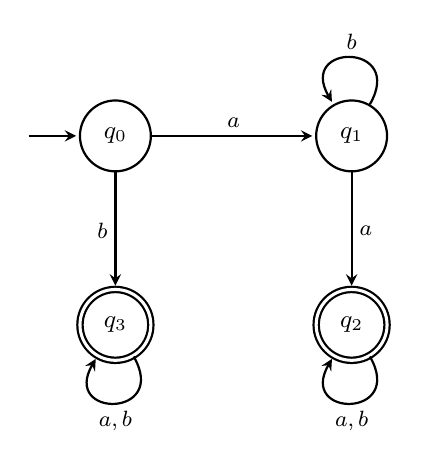
\begin{tikzpicture}
		\node[sta] (q0) at (0,1.4) {$q_0$};
		\node[sta] (q1) at (3,1.4) {$q_1$};
		\node[acc] (q2) at (3,-1.0) {$q_2$};
		\node[acc] (q3) at (0,-1.0) {$q_3$};
		\initarr{q0}{(-1.1,0)}
		\draw[tra] (q0) -- node[tlab, above] {$a$} (q1);
		\draw[tra] (q0) -- node[tlab, left] {$b$} (q3);
		\draw[tra] (q1) -- node[tlab, right] {$a$} (q2);
		\draw[tra] (q1) to[out=60, in=120, looseness=5] node[tlab, above] {$b$} (q1);
		\draw[tra] (q2) to[out=-60, in=-120, looseness=5] node[tlab, below] {$a,b$} (q2);
		\draw[tra] (q3) to[out=-60, in=-120, looseness=5] node[tlab, below] {$a,b$} (q3);
	\end{tikzpicture}
	\end{center}
	After initialisation, the pairs involving exactly one of the accept states $q_2, q_3$ are marked with $\eps$:
	\begin{center}
	\begin{tabular}{c|cccc}
		& $q_0$ & $q_1$ & $q_2$ & $q_3$ \\\hline
		$q_0$ & & & $\eps$ & $\eps$ \\
		$q_1$ & & & $\eps$ & $\eps$ \\
		$q_2$ & & & & \\
		$q_3$ & & & &
	\end{tabular}
	\end{center}
	In the first sweep, $\delta(q_0,a) = q_1$ and $\delta(q_1,a) = q_2$, and the entry $A_{q_1,q_2}$ is marked, so we mark $A_{q_0,q_1}$ with $a$:
	\begin{center}
	\begin{tabular}{c|cccc}
		& $q_0$ & $q_1$ & $q_2$ & $q_3$ \\\hline
		$q_0$ & & $a$ & $\eps$ & $\eps$ \\
		$q_1$ & & & $\eps$ & $\eps$ \\
		$q_2$ & & & & \\
		$q_3$ & & & &
	\end{tabular}
	\end{center}
	The only remaining blank is $A_{q_2,q_3}$, and it stays blank: both $q_2$ and $q_3$ are absorbing accept states, so $\delta(q_2,a) = q_2$, $\delta(q_3,a) = q_3$ and the entry $A_{q_2,q_3}$ can only ever be filled from itself. So $q_2 \sim q_3$, and the minimal automaton has three states $[q_0], [q_1], [q_2]$.

	It is illuminating to read the same computation backwards, as a \vocab{refinement of partitions}. We begin with the partition of $Q$ into one block, and each time an entry is filled we split the block containing that pair:
	\begin{center}
	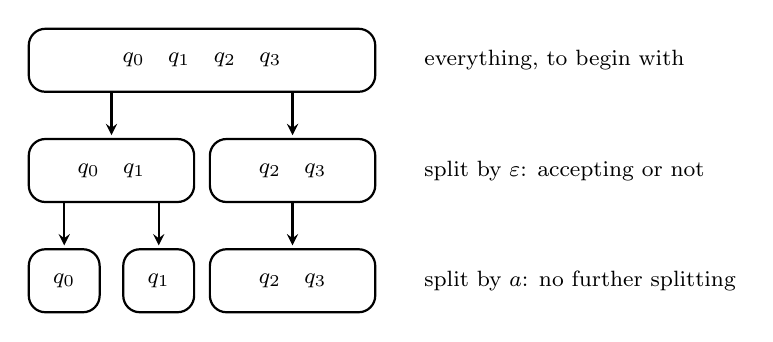
\begin{tikzpicture}[font=\footnotesize,
		bl/.style={blob, minimum height=0.8cm, inner sep=3pt}]
		\node[bl, minimum width=4.4cm] (L0) at (0,2.5) {$q_0\quad q_1\quad q_2\quad q_3$};
		\node[bl, minimum width=2.1cm] (A1) at (-1.15,1.1) {$q_0\quad q_1$};
		\node[bl, minimum width=2.1cm] (B1) at (1.15,1.1) {$q_2\quad q_3$};
		\node[bl, minimum width=0.9cm] (A2) at (-1.75,-0.3) {$q_0$};
		\node[bl, minimum width=0.9cm] (B2) at (-0.55,-0.3) {$q_1$};
		\node[bl, minimum width=2.1cm] (C2) at (1.15,-0.3) {$q_2\quad q_3$};
		\draw[tra] (-1.15,2.1) -- (A1);
		\draw[tra] (1.15,2.1) -- (B1);
		\draw[tra] (-1.75,0.7) -- (A2);
		\draw[tra] (-0.55,0.7) -- (B2);
		\draw[tra] (1.15,0.7) -- (C2);
		\node[anchor=west] at (2.7,2.5) {everything, to begin with};
		\node[anchor=west] at (2.7,1.1) {split by $\eps$: accepting or not};
		\node[anchor=west] at (2.7,-0.3) {split by $a$: no further splitting};
	\end{tikzpicture}
	\end{center}
	The process must stop, since each round strictly refines the partition and $Q$ is finite; when it stops, the blocks are exactly the $\sim$-classes. (Directly: $\lang(D) = \lang(b(a+b)^\star + ab^\star a(a+b)^\star)$, and one can check by hand that the three classes are `nothing decided yet', `an $a$ has been seen', and `accepted forever'.)
\end{example}

\begin{corollary}\label{cor:regequivalence}
	The equivalence problem for regular grammars is solvable.
\end{corollary}

\begin{proof}
	Given regular grammars $G, G'$, construct deterministic automata for them; delete inaccessible states, which we can identify; and quotient by $\sim$, which we can compute by Theorem~\ref{thm:tablefilling}. This yields irreducible automata $I, I'$. Now $\lang(G) = \lang(G')$ if and only if $I \cong I'$ by Theorems~\ref{thm:irreducibleexists} and~\ref{thm:irreducibleunique}, and since $I$ and $I'$ are finite there are only finitely many candidate bijections to test.
\end{proof}

For regular languages, then, everything is as good as it could be: all the closure properties hold, all three decision problems are solvable, and there is a canonical smallest machine. As we ascend the hierarchy, each of these will fail in turn.

\section{Context-Free Languages}\label{sec:cfl}

We move one step up. A context-free rule replaces a single variable $A$ by an arbitrary nonempty string, with no restriction on the shape of the right-hand side. We already know from Example~\ref{ex:0k1knotregular} that this buys us something, since $\{0^k1^k \mid k > 0\}$ is generated by the context-free grammar
$$S \to 0S1, \qquad S \to 01$$
but is not regular. The essential new feature is that a context-free derivation is no longer linear. In a regular grammar every intermediate string had the form $wA$, so a derivation was a list; here several variables can be present at once, and the natural object recording a derivation is a tree.

\subsection{Trees}

We set up trees in the way that is most convenient for the arguments below, namely as sets of finite sequences of naturals: a node is identified with the route taken to reach it from the root.

\begin{definition}[Tree]
	A set $T \subseteq \N^\star$ is a \vocab{(finitely branching) tree} if it is closed under initial segments, and for every $t \in T$ there is a \vocab{branching number} $n \in \N$ such that $tk \in T$ if and only if $k < n$.

	The empty sequence is the \vocab{root}, and lies in every nonempty tree. A node with branching number $0$ is a \vocab{leaf}. The \vocab{level} of $t$ is $\abs{t}$, and if $T$ is finite the maximum level is the \vocab{height} of $T$. The \vocab{branch} to $t$ is the sequence $t\restriction_0, t\restriction_1, \dots, t\restriction_{\abs{t}} = t$ of its initial segments.
\end{definition}

\begin{example}
	The set $T = \{\eps, 0, 1, 2, 00, 01, 10, 20, 000, 001, 0010\}$ is a tree, drawn below with the root at the top.
	\begin{center}
	\begin{tikzpicture}[level distance=1.05cm, sibling distance=1.6cm, every node/.style={font=\footnotesize}]
		\node (r) at (0,0) {$\eps$};
		\node (n0) at (-2.2,-1.05) {$0$};
		\node (n1) at (0,-1.05) {$1$};
		\node (n2) at (2.2,-1.05) {$2$};
		\node (n00) at (-3.2,-2.1) {$00$};
		\node (n01) at (-1.4,-2.1) {$01$};
		\node (n10) at (0,-2.1) {$10$};
		\node (n20) at (2.2,-2.1) {$20$};
		\node (n000) at (-3.8,-3.15) {$000$};
		\node (n001) at (-2.6,-3.15) {$001$};
		\node (n0010) at (-2.6,-4.2) {$0010$};
		\draw (r) -- (n0); \draw (r) -- (n1); \draw (r) -- (n2);
		\draw (n0) -- (n00); \draw (n0) -- (n01);
		\draw (n1) -- (n10); \draw (n2) -- (n20);
		\draw (n00) -- (n000); \draw (n00) -- (n001);
		\draw (n001) -- (n0010);
	\end{tikzpicture}
	\end{center}
	Its height is $4$; its leaves are $01$, $10$, $20$, $000$ and $0010$; and the branch to $0010$ is $\eps$, $0$, $00$, $001$, $0010$.
\end{example}

\begin{definition}[Subtree]
	For $t \in T$, the \vocab{subtree at $t$} is $T_t = \{s \mid ts \in T\}$, which is again a tree.
\end{definition}

\begin{definition}[Left-to-right order]
	Define $t < s$ for $t \neq s$ in $T$ if, letting $k_0$ be least with $t(k_0) \neq s(k_0)$ (assuming such $k_0$ exists), we have $t(k_0) < s(k_0)$.
\end{definition}

This is a partial order: it does not compare two nodes lying on the same branch, such as $0$ and $00$. It does, however, totally order the nodes at any fixed level, and in particular it totally orders the leaves. Reading the leaves in this order is what turns a tree into a string.

\subsection{Parse Trees}

\begin{definition}[Parse tree]
	Let $G = (\Sigma,V,P,S)$ be a context-free grammar. A pair $\mathbb{T} = (T,\ell)$ is a \vocab{$G$-parse tree} if $T$ is a finite tree and $\ell \colon T \to \Omega$ is a \vocab{labelling} such that
	\begin{enumerate}[label=(\roman*)]
		\item $\ell(\eps) \in V$, and we say that $\mathbb{T}$ \vocab{starts with} $\ell(\eps)$;
		\item if $\ell(t) \in \Sigma$ then $t$ is a leaf;
		\item if $\ell(t) = A \in V$ and $t$ has branching number $n+1$, then $A \to \ell(t0)\ell(t1)\cdots\ell(tn)$ is a rule of $P$.
	\end{enumerate}
	If $t_0 < t_1 < \cdots < t_m$ are the leaves of $T$ in left-to-right order, the \vocab{string parsed by $\mathbb{T}$} is
	$$\sigma_{\mathbb{T}} = \ell(t_0)\ell(t_1)\cdots\ell(t_m).$$
\end{definition}

Note that a variable labelling a node of branching number $0$ is permitted; such a leaf contributes a variable to $\sigma_{\mathbb{T}}$, and corresponds to a derivation that has not been finished. If $t \in T$, splitting the leaves into those to the left of $t$, those below $t$ and those to the right of $t$ gives
$$\sigma_{\mathbb T} = \alpha\, \sigma_{\mathbb T_t}\, \beta$$
for some strings $\alpha,\beta$, where $\mathbb T_t = (T_t, \ell_t)$ with $\ell_t(s) = \ell(ts)$.

\begin{example}\label{ex:parsetree}
	Let $G$ be the grammar $S \to 0S1 \mid 01$ over $\Sigma = \{0,1\}$. The parse tree for $000111$ is the following.
	\begin{center}
	\begin{tikzpicture}[every node/.style={font=\small}]
		\node (s1) at (0,3.15) {$S$};
		\node (a1) at (-1.7,2.1) {$0$};
		\node (s2) at (0,2.1) {$S$};
		\node (b1) at (1.7,2.1) {$1$};
		\node (a2) at (-1.0,1.05) {$0$};
		\node (s3) at (0,1.05) {$S$};
		\node (b2) at (1.0,1.05) {$1$};
		\node (a3) at (-0.45,0) {$0$};
		\node (b3) at (0.45,0) {$1$};
		\draw (s1) -- (a1); \draw (s1) -- (s2); \draw (s1) -- (b1);
		\draw (s2) -- (a2); \draw (s2) -- (s3); \draw (s2) -- (b2);
		\draw (s3) -- (a3); \draw (s3) -- (b3);
	\end{tikzpicture}
	\end{center}
	Its leaves in left-to-right order are the six letters $0,0,0,1,1,1$, so $\sigma_{\mathbb T} = 000111$ as promised. The corresponding derivation is $S \Rightarrow 0S1 \Rightarrow 00S11 \Rightarrow 000111$.
\end{example}

\begin{proposition}\label{prop:parsetreeiff}
	Let $G$ be context-free and $w \in \WW$. Then $w \in \lang(G)$ if and only if there is a $G$-parse tree $\mathbb T$ starting with $S$ and with $\sigma_{\mathbb T} = w$.
\end{proposition}

\begin{proof}
	Call a sequence $\mathbb T_0, \dots, \mathbb T_n$ of $G$-parse trees \vocab{derivative} if $\mathbb T_0 = (\{\eps\}, \eps \mapsto S)$, and each $\mathbb T_{i+1}$ is obtained from $\mathbb T_i$ by choosing a leaf $t$ with $\ell_i(t) = A \in V$ and a rule $A \to x_0\cdots x_n \in P$, and adjoining successors $t0, \dots, tn$ with $\ell_{i+1}(tk) = x_k$.

	Derivative sequences correspond exactly to derivations from $S$: adjoining the successors of $t$ replaces the occurrence of $A$ contributed by $t$ in $\sigma_{\mathbb T_i}$ by $x_0\cdots x_n$, and leaves the rest of the string alone, which is precisely one application of $A \to x_0\cdots x_n$. Hence $\sigma_{\mathbb T_0} \Rightarrow_G \sigma_{\mathbb T_1} \Rightarrow_G \cdots \Rightarrow_G \sigma_{\mathbb T_n}$, and conversely each derivation determines such a sequence by recording where each rule was applied.

	So if there is a derivative sequence ending at $\mathbb T$, then $S \Rightarrow_G^\star \sigma_{\mathbb T}$. It remains to show every parse tree $\mathbb T$ starting with $S$ arises this way. Set $\mathbb T_0$ to be the one-node tree. Given $\mathbb T_i$ with $T_i \subsetneq T$, pick $t \in T \setminus T_i$ of minimal length; then its predecessor $t\restriction_{\abs{t}-1}$ is a leaf of $T_i$ but not of $T$, and is labelled by a variable, so we may adjoin all of its $T$-successors to form $T_{i+1}$. Since $T$ is finite this terminates with $T_n = T$, giving a derivative sequence.
\end{proof}

The following surgery on parse trees will be needed for the pumping lemma.

\begin{definition}[Grafting]
	Let $\mathbb T = (T,\ell)$ be a parse tree, $t \in T$ with $\ell(t) = A$, and $\mathbb T' = (T', \ell')$ a parse tree starting with $A$. Then $\graft(\mathbb T, t, \mathbb T') = (S,\ell^\star)$ where
	$$S = \{s \in T \mid t \not\subseteq s\} \cup \{tu \mid u \in T'\}, \qquad \ell^\star(s) = \begin{cases}\ell(s) & t \not\subseteq s,\\ \ell'(u) & s = tu,\; u \in T'.\end{cases}$$
\end{definition}

That is, we cut off the subtree at $t$ and glue $\mathbb T'$ in its place; the result is again a parse tree, because the only condition involving $t$ is that the rule applied at $t$ matches its successors, and this is inherited from $\mathbb T'$. If $\sigma_{\mathbb T} = \alpha\sigma_{\mathbb T_t}\beta$ then
$$\sigma_{\graft(\mathbb T, t, \mathbb T')} = \alpha\, \sigma_{\mathbb T'}\, \beta.$$

\subsection{Ambiguity}

A word may have several parse trees, and this matters a great deal in practice, since the parse tree of a program is what determines its meaning.

\begin{definition}
	A context-free grammar $G$ is \vocab{ambiguous} if some $w \in \lang(G)$ has two distinct parse trees starting with $S$.
\end{definition}

\begin{example}
	Let $\Sigma = \{a,+,\ast,(,)\}$, $V = \{E\}$ and
	$$E \to E+E \mid E \ast E \mid (E) \mid a.$$
	The word $a+a\ast a$ has the two parse trees
	\begin{center}
	\begin{tikzpicture}[every node/.style={font=\small}, scale=0.92, transform shape]
		\begin{scope}
		\node (e) at (0,3) {$E$};
		\node (l) at (-1.5,2) {$E$};
		\node (p) at (0,2) {$+$};
		\node (r) at (1.5,2) {$E$};
		\node (la) at (-1.5,1) {$a$};
		\node (rl) at (0.7,1) {$E$};
		\node (rm) at (1.5,1) {$\ast$};
		\node (rr) at (2.3,1) {$E$};
		\node (rla) at (0.7,0) {$a$};
		\node (rra) at (2.3,0) {$a$};
		\draw (e) -- (l); \draw (e) -- (p); \draw (e) -- (r);
		\draw (l) -- (la);
		\draw (r) -- (rl); \draw (r) -- (rm); \draw (r) -- (rr);
		\draw (rl) -- (rla); \draw (rr) -- (rra);
		\end{scope}
		\begin{scope}[xshift=7.2cm]
		\node (e) at (0,3) {$E$};
		\node (l) at (-1.5,2) {$E$};
		\node (p) at (0,2) {$\ast$};
		\node (r) at (1.5,2) {$E$};
		\node (ll) at (-2.3,1) {$E$};
		\node (lm) at (-1.5,1) {$+$};
		\node (lr) at (-0.7,1) {$E$};
		\node (lla) at (-2.3,0) {$a$};
		\node (lra) at (-0.7,0) {$a$};
		\node (ra) at (1.5,1) {$a$};
		\draw (e) -- (l); \draw (e) -- (p); \draw (e) -- (r);
		\draw (l) -- (ll); \draw (l) -- (lm); \draw (l) -- (lr);
		\draw (ll) -- (lla); \draw (lr) -- (lra);
		\draw (r) -- (ra);
		\end{scope}
	\end{tikzpicture}
	\end{center}
	both parsing $a+a\ast a$. The left tree groups the expression as $a + (a \ast a)$ and the right as $(a+a)\ast a$; if the letters were numbers these would evaluate differently. So $G$ is ambiguous. One can find an unambiguous grammar for the same language by introducing variables for `term' and `factor', which is what forces the usual precedence rules; but there are context-free languages for which \emph{every} grammar is ambiguous, and these are called \vocab{inherently ambiguous}.
\end{example}

\subsection{Chomsky Normal Form}

Parse trees for general context-free grammars can have arbitrarily large branching, which makes counting arguments awkward. It is therefore very convenient that we may always assume the branching is at most $2$.

\begin{definition}[Chomsky normal form]
	A grammar is in \vocab{Chomsky normal form} if every rule is of the form $A \to BC$ with $B, C \in V$ (a \vocab{binary} rule) or $A \to a$ with $a \in \Sigma$ (a \vocab{unary} rule).
\end{definition}

Every grammar in Chomsky normal form is context-free. In such a grammar, parse trees are binary and derivations have a fixed length.

\begin{lemma}\label{lem:cnflength}
	Let $G$ be in Chomsky normal form and $w \in \lang(G)$ with $\abs{w} = n$. Then every $G$-derivation of $w$ from $S$ has length exactly $2n - 1$.
\end{lemma}

\begin{proof}
	A binary rule increases the length by one and the variable count by one; a unary rule leaves the length alone and decreases the variable count by one. We begin with the string $S$, of length $1$ with one variable, and end with $w$, of length $n$ with no variables. If $p$ binary and $q$ unary rules are used, then $1 + p = n$ and $1 + p - q = 0$, so $p = n-1$ and $q = n$, giving $2n-1$ steps.
\end{proof}

\begin{theorem}[Chomsky]\label{thm:cnf}
	Every context-free grammar is equivalent to one in Chomsky normal form, and such a grammar can be computed from the original.
\end{theorem}

\begin{proof}
	There are three kinds of rule obstructing Chomsky normal form:
	\begin{enumerate}[label=(\alph*)]
		\item rules $A \to \alpha$ with $\abs{\alpha} \geq 2$ where $\alpha$ contains a letter;
		\item rules $A \to B$ with $B \in V$, called \vocab{unit rules};
		\item rules $A \to \alpha$ with $\abs{\alpha} > 2$ where $\alpha$ contains only variables.
	\end{enumerate}
	We remove them in turn.

	\emph{(a)} For each $a \in \Sigma$ introduce a fresh variable $X_a$ and the rule $X_a \to a$, and replace every offending rule $A \to \alpha$ by $A \to X(\alpha)$, where $X$ replaces each letter $a$ by $X_a$. This is exactly the construction of Lemma~\ref{lem:variablebased} applied to the right-hand sides, and the same argument shows the language is unchanged. Afterwards, the only rules whose right-hand side contains a letter are the unary rules.

	\emph{(b)} Call $G$ \vocab{unit closed} if whenever $A \to B$ and $B \to \alpha$ lie in $P$, so does $A \to \alpha$. Every grammar can be made unit closed by repeatedly adding such rules; at most $\abs{V}\cdot\abs{P}$ new rules can be added, so this terminates, and it clearly does not change the language.

	Now suppose $G$ is unit closed, and let $G'$ be $G$ with all unit rules deleted. Certainly $\lang(G') \subseteq \lang(G)$. Conversely let $w \in \lang(G)$ and take a $G$-derivation of $w$ of minimal length. Suppose it uses a unit rule, and consider the \emph{last} such use:
	$$S \Rightarrow_G^\star \alpha A\beta \Rightarrow_G \alpha B \beta \Rightarrow_G^\star w.$$
	Since $w$ contains no variables, the occurrence of $B$ just created must eventually be rewritten; let
	$$S \Rightarrow_G^\star \alpha A\beta \Rightarrow_G \alpha B\beta \Rightarrow_G^\star \gamma B \delta \Rightarrow_G \gamma\zeta\delta \Rightarrow_G^\star w$$
	where $B \to \zeta$ is the first rule applied to that occurrence. The segment $\alpha B \beta \Rightarrow^\star_G \gamma B \delta$ does not touch that occurrence of $B$, so the same rules apply verbatim to $\alpha A \beta$, giving $\alpha A \beta \Rightarrow_G^\star \gamma A \delta$. By unit closure $A \to \zeta \in P$, so we may continue $\gamma A \delta \Rightarrow_G \gamma \zeta \delta$, and we have produced a strictly shorter derivation of $w$ -- contradicting minimality. Hence the minimal derivation uses no unit rule, and is a $G'$-derivation.

	\emph{(c)} Finally consider $A \to A_1A_2\cdots A_n$ with $n > 2$ and all $A_i \in V$. Introduce fresh variables $X_1, \dots, X_{n-2}$ and replace this rule by
	$$A \to A_1X_1, \quad X_1 \to A_2X_2, \quad \dots, \quad X_{n-3}\to A_{n-2}X_{n-2}, \quad X_{n-2} \to A_{n-1}A_n.$$
	The new variables occur in no other rule, so the only strings derivable using them are the intermediate stages of the replacement, and the language is unchanged.

	Applying (a), then (b), then (c) leaves only binary and unary rules.
\end{proof}

\subsection{The Pumping Lemma for Context-Free Languages}

The pumping lemma for regular languages came from a repeated state on a path. Its analogue here comes from a repeated \emph{variable} on a branch of a parse tree, and the resulting pump has two pieces -- one on either side of the repeated subtree.

\begin{definition}
	A language $L$ satisfies the \vocab{context-free pumping lemma with pumping number $n$} if every $w \in L$ with $\abs{w} \geq n$ can be written $w = xuyvz$ with
	$$\abs{uyv} \leq n, \qquad \abs{uv} > 0, \qquad xu^kyv^kz \in L \text{ for all } k \in \N.$$
	We call the pair $(u,v)$ the \vocab{pump}.
\end{definition}

\begin{remark}
	Note the differences from the regular version. The pump has two parts, of which one may be empty (only their total length is required to be positive). There is no constraint on where the pump sits in the word: $x$ and $z$ may be arbitrarily long. But the pump together with the material between its two halves is bounded.

	If $L$ satisfies the regular pumping lemma with number $n$ then it satisfies the context-free one with the same $n$, taking $v = \eps$; so by Example~\ref{ex:pumpingnotsufficient} there are uncountably many languages satisfying the context-free pumping lemma, and it cannot possibly characterise the countably many context-free languages.
\end{remark}

\begin{theorem}\label{thm:cfpumping}
	Every context-free language satisfies the context-free pumping lemma for some $n$.
\end{theorem}

\begin{proof}
	Let $L$ be context-free. By Theorem~\ref{thm:cnf} take a Chomsky normal form grammar $G$ with $\lang(G) = L$, put $m = \abs{V}$ and $n = 2^m$.

	\emph{Claim: if $\mathbb T$ is a $G$-parse tree of height $h+1$ whose string is a word, then $\abs{\sigma_{\mathbb T}} \leq 2^h$.} Since every node has branching number $1$ or $2$, and since $\sigma_{\mathbb T}$ is a word, the leaves are exactly the nodes labelled by letters and each arises from a unary rule applied to its parent. Deleting the leaves therefore gives a binary tree of height $h$, whose leaves are the parents; there are at most $2^h$ of these, and each has exactly one child. So $\abs{\sigma_{\mathbb T}} \leq 2^h$.

	Now let $w \in L$ with $\abs{w} \geq 2^m$ and let $\mathbb T$ be a parse tree for $w$. By the claim, the height of $\mathbb T$ is at least $m+1$. Let $t$ be a node at maximal level, so the branch to $t$ has $h+1 \geq m+2$ nodes; all but the last are labelled by variables, the last by a letter.

	Let $s$ be the node on that branch for which the subtree $\mathbb T_s$ has height exactly $m+1$. By the claim, $\abs{\sigma_{\mathbb T_s}} \leq 2^m = n$. The portion of the branch from $s$ to $t$ has $m+2$ nodes, of which $m+1$ are labelled by variables; as there are only $m$ variables, by pigeonhole two of them carry the same label. Say $t_0 \subsetneq t_1$ lie on this branch with $\ell(t_0) = \ell(t_1) = A$.

	Decompose the string according to these nodes:
	$$\sigma_{\mathbb T} = x'\,\sigma_{\mathbb T_s}\,z', \qquad \sigma_{\mathbb T_s} = x''\,\sigma_{\mathbb T_{t_0}}\,z'', \qquad \sigma_{\mathbb T_{t_0}} = u\,\sigma_{\mathbb T_{t_1}}\,v, \qquad \sigma_{\mathbb T_{t_1}} = y,$$
	and set $x = x'x''$ and $z = z''z'$, so that $w = xuyvz$. Since $\sigma_{\mathbb T_{t_0}} = uyv$ is a substring of $\sigma_{\mathbb T_s}$, we get $\abs{uyv} \leq n$. And $t_0 \neq t_1$ with $G$ in Chomsky normal form means the subtree at $t_0$ strictly contains that at $t_1$ together with at least one further leaf, so $\abs{uv} > 0$.
	\begin{center}
	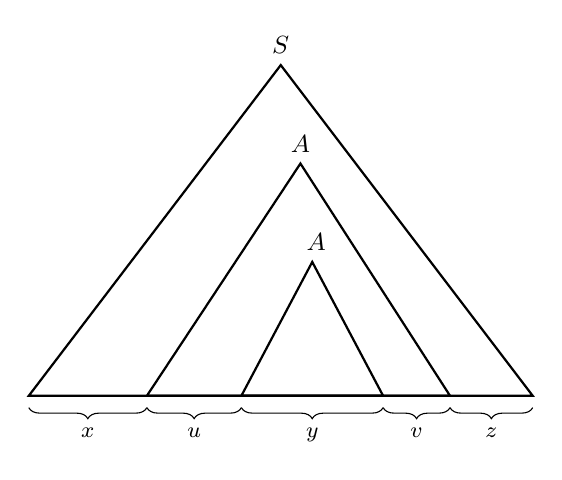
\begin{tikzpicture}[every node/.style={font=\small}]
		\draw[thick] (0,4.2) -- (-3.2,0) -- (3.2,0) -- cycle;
		\node at (0,4.45) {$S$};
		\draw[thick] (0.25,2.95) -- (-1.7,0) -- (2.15,0) -- cycle;
		\node at (0.25,3.2) {$A$};
		\draw[thick] (0.4,1.7) -- (-0.5,0) -- (1.3,0) -- cycle;
		\node at (0.45,1.95) {$A$};
		\draw[decorate, decoration={brace, amplitude=4pt, mirror}] (-3.2,-0.15) -- node[below=4pt, font=\footnotesize] {$x$} (-1.7,-0.15);
		\draw[decorate, decoration={brace, amplitude=4pt, mirror}] (-1.7,-0.15) -- node[below=4pt, font=\footnotesize] {$u$} (-0.5,-0.15);
		\draw[decorate, decoration={brace, amplitude=4pt, mirror}] (-0.5,-0.15) -- node[below=4pt, font=\footnotesize] {$y$} (1.3,-0.15);
		\draw[decorate, decoration={brace, amplitude=4pt, mirror}] (1.3,-0.15) -- node[below=4pt, font=\footnotesize] {$v$} (2.15,-0.15);
		\draw[decorate, decoration={brace, amplitude=4pt, mirror}] (2.15,-0.15) -- node[below=4pt, font=\footnotesize] {$z$} (3.2,-0.15);
	\end{tikzpicture}
	\end{center}

	Finally we pump. Both $\mathbb T_{t_0}$ and $\mathbb T_{t_1}$ are parse trees starting with $A$, so grafting is available. Set
	$$\mathbb T_{(0)} = \mathbb T_{t_1}, \qquad \mathbb T_{(i+1)} = \graft(\mathbb T_{t_0},\, t_1,\, \mathbb T_{(i)}),$$
	so that by induction $\sigma_{\mathbb T_{(i)}} = u^iyv^i$. Then $\graft(\mathbb T,\, t_0,\, \mathbb T_{(k)})$ is a parse tree starting with $S$ whose string is $xu^kyv^kz$, so $xu^kyv^kz \in L$ for every $k$. (For $k = 0$ this is grafting $\mathbb T_{t_1}$ in place of $\mathbb T_{t_0}$, which is the `pump down'.)
\end{proof}

\begin{example}\label{ex:anbncn}
	The language $L = \{a^nb^nc^n \mid n > 0\}$ is not context-free.

	Suppose it were, with pumping number $N$. Consider $a^Nb^Nc^N \in L$ and write it as $xuyvz$ with $\abs{uyv} \leq N$ and $\abs{uv} > 0$. Since $uyv$ is a substring of length at most $N$, and the blocks of $a$'s, $b$'s and $c$'s each have length $N$, the substring $uyv$ cannot contain letters of all three kinds. Pumping up to $k = 2$ increases the number of occurrences of at least one letter (as $\abs{uv} > 0$) but leaves the count of at least one other letter unchanged. The result is therefore not of the form $a^mb^mc^m$, contradiction.
\end{example}

\begin{remark}
	The language $\{a^nb^nc^n\}$ \emph{is} context-sensitive; a grammar for it may be built from rules such as $S \to abc \mid aAbc$, $Ab \to bA$, $Ac \to Bbcc$, $bB \to Bb$, $aB \to aa \mid aaA$, and one checks that this generates exactly $L$. So the inclusion of type $2$ in type $1$ is strict, as drawn in our picture of the hierarchy.
\end{remark}

\subsection{Closure Properties}

The context-free languages inherit closure under union and concatenation from Theorem~\ref{thm:closureunionconcat}, since context-free grammars are variable-based and the added rules $T \to SS'$, $T \to S$, $T \to S'$ are context-free. They are also closed under Kleene plus: given $G$, take a fresh $T$ and put $T \to S \mid TS$.

The good news stops there.

\begin{proposition}\label{prop:cfnotintersection}
	The context-free languages are not closed under intersection, complement or difference.
\end{proposition}

\begin{proof}
	Let
	$$L_0 = \{a^nb^nc^k \mid n,k > 0\}, \qquad L_1 = \{a^kb^nc^n \mid n,k > 0\}.$$
	Both are context-free: $L_0$ is the concatenation of $\{a^nb^n\}$ and $\{c^k\}$, and $L_1$ is the concatenation of $\{a^k\}$ and $\{b^nc^n\}$, and each factor is context-free: the two-letter blocks by the grammar of Example~\ref{ex:parsetree} with the letters renamed, and $\{c^k\}$ and $\{a^k\}$ by regular grammars. But $L_0 \cap L_1 = \{a^nb^nc^n \mid n > 0\}$, which is not context-free by Example~\ref{ex:anbncn}.

	Since the class is closed under union, closure under complement would give closure under intersection by De Morgan; so complement fails too, as does difference, since $L \cap M = L \setminus (L \setminus M)$.
\end{proof}

This has an important consequence for the machine model we are about to meet: \emph{whatever} machines characterise the context-free languages, there can be no product construction for them. Two such machines cannot in general be run side by side on the same input. In hindsight the reason is easy to see, and it is that the machine will have an unbounded memory, so the pair of memories cannot be packaged into a single memory of the same kind.

\subsection{Pushdown Automata}

We describe, without proofs, the machine model corresponding to context-free languages. A \vocab{pushdown automaton} is a finite automaton equipped with a \vocab{stack}: an unbounded sequence of symbols of which only the topmost is visible. Two operations are available, \vocab{push} (place a new symbol on top) and \vocab{pop} (remove the topmost symbol). There is no random access; a symbol placed on the stack can only be read after everything placed on top of it has been removed, so symbols come off in the reverse of the order in which they went on.

\begin{center}
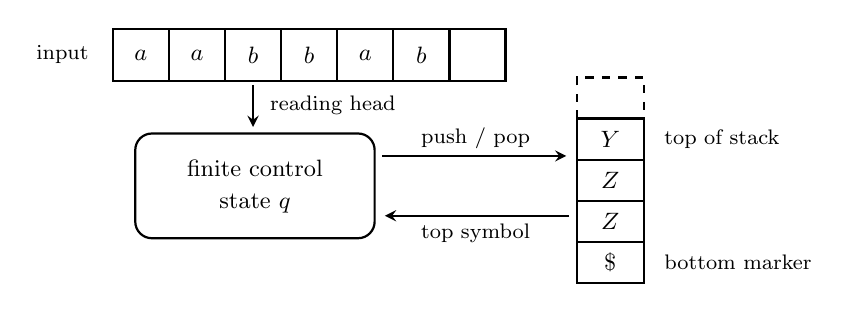
\begin{tikzpicture}[scale=0.95, transform shape]
	% input tape
	\foreach \i/\s in {0/a, 1/a, 2/b, 3/b, 4/a, 5/b, 6/{}} {
		\draw[thick] (\i*0.75, 3.3) rectangle (\i*0.75+0.75, 4.0);
		\node[font=\small] at (\i*0.75+0.375, 3.65) {$\s$};
	}
	\node[font=\footnotesize, anchor=east] at (-0.2,3.65) {input};
	\draw[tra] (1.875,3.25) -- (1.875,2.65);
	\node[font=\footnotesize, anchor=west] at (1.98,2.98) {reading head};
	% control
	\draw[blob, fill=none] (0.3,1.2) rectangle (3.5,2.6);
	\node[font=\small] at (1.9,2.14) {finite control};
	\node[font=\small] at (1.9,1.66) {state $q$};
	% stack (bottom marker at the bottom, room to grow at the top)
	\draw[thick, dashed] (6.2,2.80) rectangle (7.1,3.35);
	\foreach \i/\s in {0/{\$}, 1/{Z}, 2/{Z}, 3/{Y}} {
		\draw[thick] (6.2, \i*0.55+0.6) rectangle (7.1, \i*0.55+1.15);
		\node[font=\small] at (6.65, \i*0.55+0.875) {$\s$};
	}
	\node[font=\footnotesize, anchor=west] at (7.25,2.525) {top of stack};
	\node[font=\footnotesize, anchor=west] at (7.25,0.875) {bottom marker};
	% arrows between control and stack
	\draw[tra] (3.6,2.30) -- node[tlab, above] {push / pop} (6.1,2.30);
	\draw[tra] (6.1,1.50) -- node[tlab, below] {top symbol} (3.6,1.50);
\end{tikzpicture}
\end{center}

Formally, the transition function of such a machine takes as an extra input the symbol currently on top of the stack, and produces as an extra output an instruction to push a symbol, to pop, or to do nothing:
$$\delta \colon Q \times \Sigma \times \Gamma \longrightarrow \power\big(Q \times \Gamma^\star\big),$$
where $\Gamma$ is a finite \vocab{stack alphabet}. The machine accepts if some run consumes the whole input and finishes in an accept state.

\begin{theorem}
	A language is context-free if and only if it is accepted by a pushdown automaton.
\end{theorem}

It is worth seeing informally why the stack is exactly the right amount of extra power for $\{0^k1^k\}$. Reading the $0$s, the machine pushes one stack symbol per $0$; reading the $1$s, it pops one per $1$; and it accepts if the stack empties exactly as the input runs out. The stack cannot do this twice over -- once emptied, the information is gone -- which is the informal reason that $\{a^nb^nc^n\}$ is beyond its reach.

Note also that, unlike the case of finite automata, \emph{nondeterministic} pushdown automata are strictly more powerful than deterministic ones: the deterministic pushdown automata accept a proper subclass of the context-free languages (for example the language of even-length palindromes is context-free but not deterministic context-free). So the pleasant state of affairs of Theorem~\ref{thm:subset} does not survive the move up the hierarchy either.

\subsection{Decision Problems for Context-Free Languages}

\begin{proposition}
	The word problem for context-free grammars is solvable.
\end{proposition}

\begin{proof}
	Context-free grammars are noncontracting, so this is Corollary~\ref{cor:wordproblemsolvable}. Alternatively, and much more efficiently: convert to Chomsky normal form, whereupon by Lemma~\ref{lem:cnflength} every derivation of $w$ has length exactly $2\abs{w}-1$, and check all of them. (The standard polynomial-time algorithm, due to Cocke, Younger and Kasami, computes for each substring of $w$ the set of variables deriving it, by dynamic programming.)
\end{proof}

\begin{proposition}
	The emptiness problem for context-free grammars is solvable.
\end{proposition}

\begin{proof}
	Exactly as for regular languages. Let $n$ be a context-free pumping number for $\lang(G)$, computed as $2^{\abs{V}}$ from a Chomsky normal form grammar. If $\lang(G) \neq \varnothing$, take $w \in \lang(G)$ of minimal length; if $\abs{w} \geq n$ then $w = xuyvz$ can be pumped down to $xyz$, which is shorter and still in $\lang(G)$, a contradiction. So $\lang(G)$ is nonempty if and only if it contains a word of length less than $n$, and there are finitely many of those to test.
\end{proof}

\begin{remark}
	The equivalence problem for context-free grammars, by contrast, is \emph{unsolvable}; so is the question of whether a given context-free grammar is ambiguous, and whether the intersection of two context-free languages is empty. We shall not prove these, but the first taste of such a result is the unsolvability of the corresponding problems for type $0$ grammars in Section~\ref{sec:solvability}.
\end{remark}

We can summarise the situation so far in a table.
\begin{center}
	\begin{tabular}{l|cccc}
		& union & concatenation & intersection & complement \\\hline
		regular & yes & yes & yes & yes \\
		context-free & yes & yes & no & no
	\end{tabular}
	\qquad
	\begin{tabular}{l|ccc}
		& word & emptiness & equivalence \\\hline
		regular & yes & yes & yes \\
		context-free & yes & yes & no
	\end{tabular}
\end{center}
Everything above the line is settled; to go further we need to say what an algorithm is, and that is what we do next.

\section{Register Machines}\label{sec:rm}

We now give a precise definition of `algorithm'. The model we use is the \emph{register machine}: a finite automaton equipped not with one stack, but with finitely many. That extra freedom turns out to be all that is required to obtain full computational power.

\subsection{The Definition}

A register machine has an alphabet $\Sigma$, a finite set $Q$ of states, and finitely many \vocab{registers}, each holding a word $w \in \WW$. The machine can inspect the last letter of a register, delete it, or append a new one -- so a register behaves as a stack, with the right-hand end of the word as the top.

\begin{center}
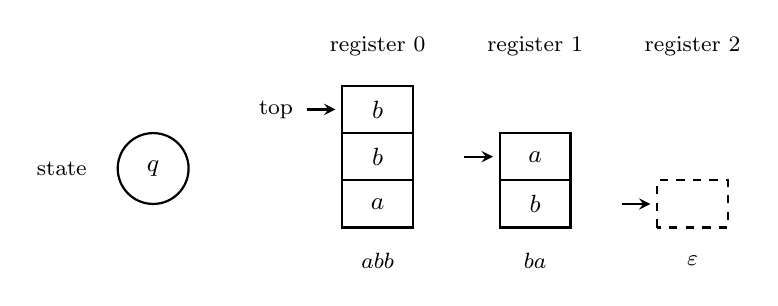
\begin{tikzpicture}
	\node[sta] (q) at (0,0.95) {$q$};
	\node[font=\footnotesize, anchor=east] at (-0.72,0.95) {state};
	% register 0 holds abb: bottom a, then b, top b
	\foreach \i/\s in {0/a, 1/b, 2/b} { \draw[reg] (2.4,\i*0.6+0.2) rectangle ++(0.9,0.6); \node[font=\small] at (2.85,\i*0.6+0.5) {$\s$}; }
	% register 1 holds ba: bottom b, top a
	\foreach \i/\s in {0/b, 1/a} { \draw[reg] (4.4,\i*0.6+0.2) rectangle ++(0.9,0.6); \node[font=\small] at (4.85,\i*0.6+0.5) {$\s$}; }
	% register 2 is empty
	\draw[reg, dashed] (6.4,0.2) rectangle ++(0.9,0.6);
	\node[font=\footnotesize] at (2.85,2.5) {register $0$};
	\node[font=\footnotesize] at (4.85,2.5) {register $1$};
	\node[font=\footnotesize] at (6.85,2.5) {register $2$};
	\node[font=\footnotesize] at (2.85,-0.22) {$abb$};
	\node[font=\footnotesize] at (4.85,-0.22) {$ba$};
	\node[font=\footnotesize] at (6.85,-0.22) {$\eps$};
	\draw[tra] (1.95,1.7) -- (2.35,1.7);
	\node[font=\footnotesize, anchor=east] at (1.9,1.7) {top};
	\draw[tra] (3.95,1.1) -- (4.35,1.1);
	\draw[tra] (5.95,0.5) -- (6.35,0.5);
\end{tikzpicture}
\end{center}

A snapshot of the whole machine is called a configuration.

\begin{definition}[Configuration]
	A \vocab{configuration} (or \vocab{snapshot}) of length $n+1$ is a tuple $(q, w_0, \dots, w_n) \in Q \times \WW^{n+1}$.
\end{definition}

One might be tempted to define the dynamics by a transition function $\delta \colon Q \times \WW^{n+1} \to Q \times \WW^{n+1}$, but this is far too permissive: there are uncountably many such functions, and they can do anything at all to the registers in one step. Instead we allow only four kinds of elementary instruction.

\begin{definition}[Instruction]
	Let $\Sigma$ be an alphabet and $Q$ a nonempty finite set of states. A \vocab{$(\Sigma,Q)$-instruction} is a tuple of one of the forms
	\begin{align*}
		(0,k,a,q) &\in \N\times\N\times\Sigma\times Q, &  (1,k,a,q,q') &\in \N\times\N\times\Sigma\times Q\times Q, \\
		(2,k,q,q') &\in \N\times\N\times Q\times Q, & (3,k,q,q') &\in \N\times\N\times Q\times Q.
	\end{align*}
	We write these more legibly as
	$$+(k,a,q), \qquad ?(k,a,q,q'), \qquad ?(k,\eps,q,q'), \qquad -(k,q,q')$$
	respectively, and we write $\Instr(\Sigma,Q)$ for the set of all of them.
\end{definition}

Their intended meanings are as follows.
\begin{itemize}
	\item $+(k,a,q)$: push the letter $a$ onto register $k$, then move to state $q$.
	\item $?(k,a,q,q')$: if the top letter of register $k$ is $a$, move to state $q$; otherwise move to $q'$.
	\item $?(k,\eps,q,q')$: if register $k$ is empty, move to state $q$; otherwise move to $q'$.
	\item $-(k,q,q')$: pop the top letter of register $k$. If the register was already empty, move to state $q$; otherwise move to $q'$.
\end{itemize}
Note that only $+$ and $-$ change the registers, and each changes exactly one register by exactly one letter.

\begin{definition}[Register machine]
	A tuple $M = (\Sigma, Q, P)$ is a \vocab{$\Sigma$-register machine} if $\Sigma$ is an alphabet, $Q$ is a finite set of states containing two distinguished states $q_S \neq q_H$ (the \vocab{start state} and the \vocab{halt state}), and
	$$P \colon Q \to \Instr(\Sigma, Q)$$
	is the \vocab{program}. Writing $Q = \{q_0, \dots, q_n\}$, we present $P$ as a finite list of \vocab{program lines} $q_i \mapsto P(q_i)$. Only finitely many register indices $k$ occur in $P$; the largest is the \vocab{upper register index} of $M$.
\end{definition}

\begin{definition}[Computation]
	Let $M$ have upper register index $m$ and let $C = (q, w_0, \dots, w_m)$ be a configuration. We say $M$ \vocab{transforms} $C$ into $C'$ if one of the following holds:
	\begin{itemize}
		\item $P(q) = +(k,a,q')$ and $C' = (q', w_0, \dots, w_{k-1}, w_ka, w_{k+1}, \dots, w_m)$;
		\item $P(q) = \,?(k,a,q',q'')$ and either $w_k = wa$ for some $w$ and $C' = (q', w_0,\dots,w_m)$, or $w_k$ does not end in $a$ and $C' = (q'', w_0,\dots,w_m)$;
		\item $P(q) = \,?(k,\eps,q',q'')$ and either $w_k = \eps$ and $C' = (q', w_0,\dots,w_m)$, or $w_k \neq \eps$ and $C' = (q'',w_0,\dots,w_m)$;
		\item $P(q) = -(k,q',q'')$ and either $w_k = \eps$ and $C' = (q', w_0,\dots,w_m)$, or $w_k = wa$ and $C' = (q'', w_0,\dots,w_{k-1},w,w_{k+1},\dots,w_m)$.
	\end{itemize}
	Given $\vv{w} \in \WW^{m+1}$, the \vocab{computation sequence} of $M$ on input $\vv{w}$ is defined by recursion:
	$$C(0,M,\vv{w}) = (q_S, \vv{w}), \qquad C(k+1,M,\vv{w}) = \text{the transform of } C(k,M,\vv{w}).$$
\end{definition}

If $\vv w$ is shorter than $m+1$ we pad it on the right with copies of $\eps$; if it is longer we simply carry the extra registers along untouched.

\begin{remark}
	Every configuration has a transform, so computation sequences as defined are always infinite. Halting is not the absence of a next step, but the arrival at a designated state.
\end{remark}

\begin{definition}[Halting]
	The computation of $M$ on input $\vv w$ \vocab{halts at time $k$} if $k$ is least with $C(k,M,\vv w) = (q_H, \vv v)$ for some $\vv v$; in this case $\vv v$ is the \vocab{output}. If no such $k$ exists, the computation \vocab{does not halt}.
\end{definition}

\subsection{Strong Equivalence}

\begin{definition}
	Register machines $M$ and $M'$ are \vocab{strongly equivalent} if for every input $\vv w$ and every $k$, the configurations $C(k,M,\vv w)$ and $C(k,M',\vv w)$ have the same register contents, and $M$ halts on $\vv w$ at time $k$ if and only if $M'$ does.
\end{definition}

So strongly equivalent machines do literally the same thing, step by step; only their state names may differ. Relabelling states shows that if $\abs{Q} = \abs{Q'}$ then every $(\Sigma,Q,P)$ has a strongly equivalent $(\Sigma,Q',P')$.

\begin{proposition}[Padding lemma]\label{prop:padding}
	Every register machine is strongly equivalent to infinitely many distinct register machines.
\end{proposition}

\begin{proof}
	Let $M = (\Sigma,Q,P)$ and add a fresh state $\hat q$ to $Q$, with $P(\hat q)$ any instruction whatsoever. Since $\hat q$ occurs in no other program line, it never appears in any computation sequence, so the resulting machine is strongly equivalent to $M$. Repeating gives infinitely many.
\end{proof}

\begin{proposition}\label{prop:countablymanyrm}
	Up to strong equivalence there are only countably many register machines over a fixed $\Sigma$.
\end{proposition}

\begin{proof}
	Up to strong equivalence only $\abs{Q}$ matters, so fix a set $Q$ with $\abs{Q} = n$ and bound the register index by $k$. Counting the four kinds of instruction,
	$$\abs{\Instr(\Sigma,Q)} = (k+1)n\abs{\Sigma} + (k+1)n^2\abs{\Sigma} + (k+1)n^2 + (k+1)n^2 =: N_{n,k},$$
	which is finite, so there are $N_{n,k}^{\,n}$ programs. The class $M_{n,k}$ of such machines is therefore finite, and every register machine lies in some $M_{n,k}$; so $\bigcup_{n,k}M_{n,k}$ is a countable union of finite sets.
\end{proof}

This is the source of all the negative results in the course. There are only countably many algorithms, and uncountably many things one might want to compute.

\subsection{Operations and Questions}

Rather than reason about programs line by line, we build up a library of things register machines can do, and thereafter argue at a higher level. There are two kinds of task.

\begin{definition}[Operation]
	An \vocab{operation} is a partial function $f \colon \WW^{m+1} \rightharpoonup \WW^{m+1}$. We write $f(\vv w)\!\downarrow$ if $\vv w \in \dom f$ (`$f$ \vocab{converges} at $\vv w$') and $f(\vv w)\!\uparrow$ otherwise (`$f$ \vocab{diverges}').

	A register machine $M$ \vocab{performs} $f$ if for every $\vv w$ we have $f(\vv w)\!\downarrow$ if and only if $M$ halts on $\vv w$, and in that case the output of $M$ is $f(\vv w)$.
\end{definition}

\begin{example}
	The operation `never halt' is the empty function. It is performed by any program which never mentions $q_H$ on the right-hand side of a line, for instance
	$$q_S \mapsto +(0,a,q_S), \qquad q_H \mapsto +(0,a,q_S).$$
	The operation `halt immediately, changing nothing' is the identity function on $\WW^{m+1}$, performed by $q_S \mapsto\, ?(0,a,q_H,q_H)$: the test is performed, both branches lead to $q_H$, and nothing is written.
\end{example}

\begin{definition}[Question]
	A \vocab{question with $k+1$ answers} is a partition of $\WW^{m+1}$ into sets $A_0, \dots, A_k$. A register machine \vocab{answers} the question if it has distinguished \vocab{answer states} $\bar q_0, \dots, \bar q_k$ such that on input $\vv w$ the computation reaches, after finitely many steps, the configuration $(\bar q_i, \vv w)$, where $i$ is the index with $\vv w \in A_i$.
\end{definition}

So a question is answered without disturbing the registers, and the answer is recorded in the state.

\begin{example}
	`Is register $i$ empty?' is answered by the single line $q_S \mapsto\, ?(i,\eps,\bar q_Y, \bar q_N)$, and `does register $i$ end in the letter $a$?' by $q_S \mapsto\, ?(i,a,\bar q_Y, \bar q_N)$.
\end{example}

The next two lemmas are what allow us to program at a high level: they say that machines can be run one after another, and that they can be selected between.

\begin{lemma}[Concatenation]\label{lem:concat}
	If $M$ performs $F$ and $M'$ performs $F'$, then there is a register machine $\hat M$ performing $F' \circ F$.
\end{lemma}

\begin{proof}
	Assume the state sets are disjoint. Let $P^\star$ be $P$ with the line for $q_H$ deleted and with every occurrence of $q_H$ replaced by $q_S'$, and set $\hat M = (\Sigma, (Q\setminus\{q_H\})\cup Q', P^\star \cup P')$, with start state $q_S$ and halt state $q_H'$. Running $\hat M$ on $\vv w$ reproduces the computation of $M$ exactly until the moment $M$ would halt, at which point $\hat M$ is in state $q_S'$ with registers $F(\vv w)$, and thereafter reproduces the computation of $M'$ on that input. So $\hat M$ halts precisely when both $F(\vv w)\!\downarrow$ and $F'(F(\vv w))\!\downarrow$, with output $F'(F(\vv w))$.
\end{proof}

\begin{lemma}[Case distinction]\label{lem:cases}
	Let $\mathsf{Q}$ be a question with answers $A_0, \dots, A_k$, answered by a machine $M$; and let $F_i$ be operations performed by machines $M_i$. Then some register machine performs
	$$G(\vv w) = F_i(\vv w) \quad\text{when } \vv w \in A_i.$$
\end{lemma}

\begin{proof}
	Assume $Q$ is disjoint from each $Q_i$ and that the $Q_i$ meet only in a common halt state $q_H$. Let $P_i^\star$ be $P_i$ with every occurrence of $q_{S,i}$ replaced by the answer state $\bar q_i$ of $M$, and delete the line for $q_{S,i}$. Put
	$$Q^\star = Q \cup \bigcup_{i\leq k}(Q_i\setminus\{q_{S,i}\}), \qquad P^\star = P \cup \bigcup_{i\leq k}P_i^\star.$$
	On input $\vv w$, the machine first runs $M$, which reaches $\bar q_i$ with the registers untouched, and from there runs $M_i$.
\end{proof}

\subsection{A Register Machine API}\label{sec:api}

We may now assemble a library of operations, each built out of the previous ones by concatenation and case distinction. A register is \vocab{unused} if no program line mentions it, and \vocab{empty} if it contains $\eps$; registers used only for intermediate work are called \vocab{scratch registers}. Since any given machine mentions only finitely many registers, an unused empty register is always available.

\begin{itemize}
	\item \emph{`Delete the last letter of register $i$'}: $q_S \mapsto -(i,q_H,q_H)$.
	\item \emph{`Push $a$ onto register $i$'}: $q_S \mapsto +(i,a,q_H)$.
	\item \emph{`Empty register $i$'}: $q_S \mapsto -(i,q_H,q_S)$. This pops repeatedly, halting exactly when the register was found to be empty.
	\item \emph{`Halt if register $i$ is nonempty, otherwise diverge'}: answer `is register $i$ empty?', then apply case distinction with the operations `never halt' and `halt immediately'.
	\item \emph{`Append the fixed word $w = a_0a_1\cdots a_\ell$ to register $i$'}: concatenate the $\ell+1$ pushes.
	\item \emph{`Replace register $i$ by the fixed word $w$'}: empty it, then append $w$.
	\item \emph{`What is the last letter of register $i$?'}: this question has $\abs{\Sigma}+1$ answers, one per letter and one for `empty'. Ask `does register $i$ end in $a_0$?'; if yes go to $\bar q_0$, if no ask about $a_1$, and so on; if every answer is no, the register is empty and we go to $\bar q_\eps$.
	\item \emph{`Copy the last letter of register $i$ onto register $j$'}: ask the previous question and push the corresponding letter in each case.
	\item \emph{`Move the last letter of register $i$ onto register $j$'}: copy it, then delete it from $i$.
	\item \emph{`Move register $i$ into register $j$ in reverse order'}: repeat the previous operation until register $i$ is empty.
	\item \emph{`Move register $i$ into register $j$ in the correct order'}: move $i$ into an unused empty register $k$ in reverse order, then move $k$ into $j$ in reverse order. Reversing twice restores the order.
	\item \emph{`Reverse register $i$'}: move it in reverse into an unused empty register, then move that back in the correct order -- or equivalently, move it out and back once each.
	\item \emph{`Move register $i$ into both $j$ and $k$ in reverse order'}: copy the last letter into $j$, then into $k$, then delete it; repeat.
	\item \emph{`Copy register $i$ into register $j$'}: move $i$ into $j$ and a scratch register $k$ simultaneously (in reverse), then move $k$ back into $i$ (in reverse). Composing with a reversal fixes the order if required.
	\item \emph{`Is register $i$ equal to the fixed word $w = a_0\cdots a_\ell$?'}: run subroutines $S_\ell$, $S_{\ell-1}$, \dots, $S_0$, where $S_r$ asks whether the last letter of register $i$ is $a_r$; if not, go to a state $q_N$; if so, move that letter to a scratch register $k$ and run $S_{r-1}$, or go to $q_Y$ if $r = 0$. At $q_N$ and at $q_Y$, move the contents of $k$ back into $i$, restoring it, and then answer $\bar q_N$ or $\bar q_Y$ as appropriate. The scratch register must be restored, since a question is not allowed to alter the registers.
\end{itemize}

It is worth writing out one of these in full, to see that the formalism really does what we claim.

\begin{example}\label{ex:rmflow}
	Take $\Sigma = \{a,b\}$. The following five-line program moves the contents of register $1$ into register $2$ in reverse order, leaving register $1$ empty.
	\begin{align*}
		q_S &\mapsto\, ?(1,a,q_a,q_1), & q_1 &\mapsto\, ?(1,b,q_b,q_H), & q_a &\mapsto +(2,a,q_2), \\
		q_b &\mapsto +(2,b,q_2), & q_2 &\mapsto -(1,q_S,q_S). &&
	\end{align*}
	As a flow diagram:
	\begin{center}
	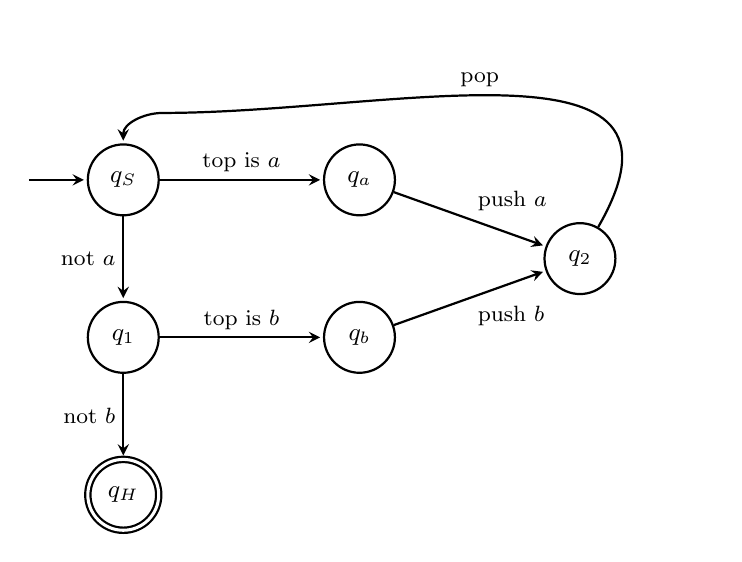
\begin{tikzpicture}
		\node[sta] (qS) at (0,0) {$q_S$};
		\node[sta] (q1) at (0,-2.0) {$q_1$};
		\node[sta] (qa) at (3.0,0) {$q_a$};
		\node[sta] (qb) at (3.0,-2.0) {$q_b$};
		\node[sta] (q2) at (5.8,-1.0) {$q_2$};
		\node[acc] (qH) at (0,-4.0) {$q_H$};
		\initarr{qS}{(-1.2,0)}
		\draw[tra] (qS) -- node[tlab, above] {top is $a$} (qa);
		\draw[tra] (qS) -- node[tlab, left] {not $a$} (q1);
		\draw[tra] (q1) -- node[tlab, above] {top is $b$} (qb);
		\draw[tra] (q1) -- node[tlab, left] {not $b$} (qH);
		\draw[tra] (qa) -- node[tlab, above right] {push $a$} (q2);
		\draw[tra] (qb) -- node[tlab, below right] {push $b$} (q2);
		\draw[tra] (q2) to[out=60,in=0, looseness=1.3] node[tlab, above, pos=0.55] {pop} (0.5,0.85) to[out=180,in=90] (qS);
	\end{tikzpicture}
	\end{center}
	Let us trace it with register $1$ containing $ab$ and register $2$ empty. In $q_S$, the top letter is $b$, not $a$, so we move to $q_1$; there the top letter is $b$, so we move to $q_b$ and push $b$ onto register $2$; in $q_2$ we pop, leaving register $1$ holding $a$, and return to $q_S$. Now the top letter is $a$, so we go to $q_a$, push $a$ onto register $2$ (which now holds $ba$), and pop, leaving register $1$ empty. Back at $q_S$: the top letter is not $a$ (the register is empty), so we go to $q_1$; it is not $b$ either, so we halt. Register $2$ holds $ba$, the reverse of $ab$, as claimed.
\end{example}

From now on we shall specify register machines by describing what they do in English, in terms of the library above, exactly as one writes a program in terms of library functions rather than machine code. This is legitimate precisely because Lemmas~\ref{lem:concat} and~\ref{lem:cases} let us assemble the pieces.

\section{Computable Functions and Sets}\label{sec:computable}

\subsection{Computable Functions}

Most computations need scratch space, and we do not want the final answer to depend on the litter left behind. So we declare that register $0$ holds the output and that everything else is scratch.

\begin{definition}
	Let $M$ be a register machine and $k \in \N$. Define $f_{M,k} \colon \WW^k \rightharpoonup \WW$ by
	$$f_{M,k}(\vv w) = \begin{cases} v_0 & \text{if } M \text{ halts on } \vv w \text{ with output } \vv v, \\ \uparrow & \text{if } M \text{ does not halt on } \vv w.\end{cases}$$
	A partial function $f \colon \WW^k \rightharpoonup \WW$ is \vocab{computable} if $f = f_{M,k}$ for some register machine $M$. For $k = 1$ we write $W_M = \dom f_{M,1}$.
\end{definition}

If $M$ and $M'$ are strongly equivalent then $f_{M,k} = f_{M',k}$, though the converse fails badly: two machines may compute the same function in completely different ways.

\begin{remark}\label{rem:countablycomputable}
	By Proposition~\ref{prop:countablymanyrm} there are only countably many computable functions, while there are uncountably many partial functions $\WW \rightharpoonup \WW$. So almost every function is not computable. On the other hand, by the padding lemma each computable function is computed by infinitely many machines. And by Lemmas~\ref{lem:concat} and~\ref{lem:cases}, computable functions are closed under composition and case distinction.
\end{remark}

\begin{example}
	The identity $\WW \to \WW$ is computable (halt immediately). Each constant function $c(\vv w) = v$ is computable (replace register $0$ by $v$). Each projection $\pi_i(\vv w) = w_i$ is computable (empty register $0$, then move register $i$ into register $0$).
\end{example}

\subsection{Computable and Computably Enumerable Sets}

To speak of computable \emph{sets} we use characteristic functions. Since our values are words rather than truth values, we fix once and for all a letter $a \in \Sigma$ to stand for `true', with $\eps$ standing for `false'.

\begin{definition}
	Let $X \subseteq \WW^k$. A total $f \colon \WW^k \to \WW$ is \vocab{a characteristic function of $X$} if $f(\vv w) \neq \eps$ exactly when $\vv w \in X$; it is \vocab{the characteristic function} $\chi_X$ if moreover $f(\vv w) = a$ for $\vv w \in X$. We call $X$ \vocab{computable} if $\chi_X$ is computable.

	A partial $f$ is \vocab{a pseudocharacteristic function of $X$} if $\dom f = X$; it is \vocab{the pseudocharacteristic function} $\psi_X$ if additionally $f(\vv w) = a$ for $\vv w \in X$. We call $X$ \vocab{computably enumerable} if $\psi_X$ is computable.
\end{definition}

A computable set is one we can \emph{decide}: given $\vv w$, the machine always halts and tells us the answer. A computably enumerable set is one we can only \emph{semi-decide}: the machine halts when the answer is yes, and runs forever when the answer is no. Since a language is a set of words, both notions apply to languages.

\begin{proposition}\label{prop:cecomputable}
	Let $X \subseteq \WW^k$.
	\begin{enumerate}[label=(\roman*)]
		\item $X$ is computable if and only if its complement is computable.
		\item $X$ is computably enumerable if and only if $X = \dom f_{M,k}$ for some register machine $M$.
		\item If $X$ is computable then $X$ is computably enumerable.
	\end{enumerate}
\end{proposition}

\begin{proof}
	Write the proof for $k = 1$; the general case is identical. By case distinction, if $g,h$ are computable then so is the function equal to $g(w)$ when $w \neq \eps$ and $h(w)$ when $w = \eps$, since `is register $0$ empty?' is answerable.

	(i) Let $f_1$ be the computable function given in this way by $g(w) = \eps$ and $h(w) = a$; that is, $f_1$ swaps $a$ and $\eps$. Then $\chi_{X^c} = f_1 \circ \chi_X$ and conversely.

	(ii) If $X = \dom f$ with $f$ computable, let $f_2$ be given by $g(w) = a$, $h(w) = a$, so $f_2$ is the total constant function $a$; then $\psi_X = f_2 \circ f$, which is computable with domain $X$. Conversely $\psi_X$ is itself computable with domain $X$.

	(iii) Let $f_3$ be given by $g(w) = a$ and $h(w) \uparrow$ (halt if register $0$ is nonempty, else diverge). Then $\psi_X = f_3 \circ \chi_X$.
\end{proof}

The converse of (iii) is false, and proving so is the content of the halting problem below. First, a sanity check that our new notion is at least as strong as the old ones.

\begin{theorem}\label{thm:regularcomputable}
	Every regular language is computable.
\end{theorem}

\begin{proof}
	Let $L = \lang(D)$ with $D = (\Sigma, Q, \delta, q_0, F)$. We describe a register machine with input in register $0$.

	First, move register $0$ into register $1$ in reverse order. (This is necessary because a register machine sees the \emph{last} letter of a word, whereas an automaton reads from the left; reversing makes the automaton's first letter the topmost.)

	For each $q \in Q$ our machine has a block of states $Q_q$, meaning `we are simulating $D$ in state $q$'. Move into $Q_{q_0}$.

	On entering $Q_q$: ask what the last letter of register $1$ is. If register $1$ is empty, move to a state $\bar q_{\mathrm{acc}}$ if $q \in F$, and to $\bar q_{\mathrm{rej}}$ otherwise. Otherwise, if the last letter is $b$, delete it and move into $Q_{\delta(q,b)}$, repeating.

	Since each pass deletes a letter, the loop terminates after $\abs{w}$ passes. At $\bar q_{\mathrm{acc}}$, empty register $0$, push $a$, and halt; at $\bar q_{\mathrm{rej}}$, empty register $0$ and halt. The resulting machine computes $\chi_L$.
\end{proof}

\subsection{The Shortlex Ordering}

Our functions take words as inputs, but recursion -- both the definition of recursive functions in Section~\ref{sec:recursive} and simple counting arguments -- needs a notion of `the next one'. We therefore transport the order type of $\N$ onto $\WW$.

\begin{definition}[Shortlex]
	Fix a total order on $\Sigma$. The \vocab{shortlex order} on $\WW$ is defined by $w < v$ if
	\begin{enumerate}[label=(\roman*)]
		\item $\abs{w} < \abs{v}$; or
		\item $\abs{w} = \abs{v}$, $w \neq v$, and at the least position where they differ, the letter of $w$ precedes that of $v$.
	\end{enumerate}
\end{definition}

So we sort by length first, and break ties lexicographically. This is a total order with least element $\eps$.

\begin{example}
	For $\Sigma = \{0,1\}$ with $0 < 1$, the shortlex order begins
	$$\eps,\; 0,\; 1,\; 00,\; 01,\; 10,\; 11,\; 000,\; 001,\; 010,\; 011,\; 100,\; 101,\; 110,\; 111,\; 0000,\; \dots$$
	Identifying each word with its index (counting from $0$), we have $\#\eps = 0$, $\#10 = 5$, $\#01 = 4$, and since $\#010 = 9 = 5 + 4$ we may write $10 + 01 = 010$. Transporting the semiring structure of $\N$ in this way makes $\WW$ into a commutative semiring; there are $\abs{\Sigma}^k$ words of length $k$, so for $\abs{\Sigma}=2$ the index of $0^k$ is $2^k - 1$.
\end{example}

\begin{theorem}
	$(\WW, <)$ is order-isomorphic to $(\N,<)$.
\end{theorem}

\begin{proof}
	For a fixed $w$ the set $\{v \mid v < w\}$ is finite, since it consists of words of length at most $\abs{w}$. So $\#(w) = \abs{\{v \mid v< w\}}$ is a well-defined function $\WW\to\N$, and it is clearly order-preserving. It is surjective, since the words listed in increasing order take every index in turn, and order-preserving maps between total orders are injective.
\end{proof}

\begin{theorem}\label{thm:successorcomputable}
	The set $\{(v,w) \mid v < w\}$ is computable, and the \vocab{successor function} $s \colon \WW \to \WW$ determined by $\#s(w) = \#w + 1$ is computable.
\end{theorem}

\begin{proof}
	To compare $v$ and $w$: copy them into scratch registers and repeatedly delete the last letter of each until one is empty; whichever empties first is shorter. If they empty simultaneously, copy them again in reverse order (so that we may read them from the left) and delete letters in step until they differ, then compare those letters in the fixed order on $\Sigma$; if no difference is found the words are equal. All of this uses only operations from Section~\ref{sec:api}.

	For the successor: locate the last letter of $w$ which is not the largest letter of $\Sigma$, replace it by its successor in $\Sigma$, and replace everything after it by copies of the least letter. If every letter of $w$ is the largest letter (including the case $w = \eps$), output the least letter repeated $\abs{w}+1$ times.
\end{proof}

\subsection{Merging and Splitting Words}

We shall repeatedly need to package a pair of words into a single word. Recall the \vocab{Cantor zigzag function}
$$z(i,j) = \frac{(i+j)(i+j+1)}{2}+j,$$
a bijection $\N\times\N\to\N$; it enumerates the lattice points of the first quadrant along successive anti-diagonals.

\begin{definition}
	For $v,w \in \WW$, the \vocab{merge} $v \ast w$ is the unique word with $\#(v\ast w) = z(\#v, \#w)$. Conversely each $w$ \vocab{splits} uniquely as $\#w = z(\#w_{(0)}, \#w_{(1)})$, and we call $w_{(0)}, w_{(1)}$ the components of $w$.
\end{definition}

Since addition and multiplication of indices are computable (they can be built from the successor function by recursion, as we will see in Section~\ref{sec:recursive}), merging is computable; strictly speaking splitting is an \emph{operation} rather than a computable function, since it has two outputs, but it is performed by a register machine which writes the components into two registers.

The point of merging is that a single existential quantifier over $\WW$ can simulate two. We shall use this so often that it acquires a name: the \vocab{zigzag argument}.

\subsection{Coding of Programs}

We now take the decisive step and treat programs as data. Let $\Sigma$ be an alphabet and let $\Sigma'$ be $\Sigma$ together with ten new symbols
$$\bm{0} \quad \bm{1} \quad \bm{+} \quad \bm{-} \quad \bm{?} \quad \bm{(} \quad \bm{)} \quad \bm{,} \quad \bm{\mapsto} \quad \bm{\square}.$$
For a mathematical object $o$ we write $\code(o) \in \Sigma'^\star$ for its code, defined as follows.
\begin{itemize}
	\item Naturals are written in binary using $\bm 0$ and $\bm 1$, so $\code(19) = \bm1\bm0\bm0\bm1\bm1$.
	\item For $Q = \{q_0, \dots, q_n\}$ we set $\code(q_k) = \code(k)$.
	\item Instructions are coded using the punctuation, for instance
	$$\code(+(k,a,\ell)) = \bm+\,\bm(\,\code(k)\,\bm,\,a\,\bm,\,\code(\ell)\,\bm),$$
	and similarly for $?$ and $-$.
	\item A program line is coded by $\code(q\mapsto I) = \code(q)\,\bm\mapsto\,\code(I)$, and a machine by listing its lines separated by $\bm,$.
	\item A tuple of words is coded by $\code(\vv w) = \bm\square w_0 \bm\square w_1 \bm\square \cdots \bm\square w_k \bm\square$, and a configuration by $\code(q,\vv w) = \code(q)\code(\vv w)$.
\end{itemize}
Not every $\Sigma'$-word is a code, but it is a purely syntactic matter to check whether a given word is one, and this check can plainly be carried out by a register machine using the operations of Section~\ref{sec:api}.

\begin{remark}
	We have enlarged the alphabet, which looks like cheating. It is not: if $\Sigma \subseteq \Sigma'$ then every $\Sigma$-machine is a $\Sigma'$-machine, and conversely one can encode each letter of $\Sigma'$ as a fixed-length block of letters of $\Sigma$ provided $\abs{\Sigma}\geq 2$, translating $\Sigma'$-machines into $\Sigma$-machines. So computability over any alphabet with at least two letters is the same notion, and we may enlarge the alphabet whenever convenient.
\end{remark}

\subsection{The Universal Register Machine}

\begin{lemma}\label{lem:stepfunction}
	The function
	$$h(w,u,v) = \begin{cases} \code\big(C(\#v, M, \vv w)\big) & \text{if } w = \code(M),\, u = \code(\vv w) \text{ for some } M, \vv w, \\ \uparrow & \text{otherwise}\end{cases}$$
	is computable.
\end{lemma}

\begin{proof}
	First check syntactically that $w$ codes a machine and $u$ codes a tuple; if not, diverge. Then define $h$ by recursion on $v$:
	$$h(w,u,\eps) = \code(q_S)\,u, \qquad h(w,u,s(v)) = \code(C'),$$
	where $C'$ is the transform, under the machine coded by $w$, of the configuration coded by $h(w,u,v)$. Computing $C'$ from $\code(C)$ and $\code(M)$ is a finite syntactic manipulation: read off the current state from $\code(C)$, look up the corresponding line of $\code(M)$, and edit the appropriate register block accordingly. All of these are operations from Section~\ref{sec:api}, and the recursion itself is available because computable functions are closed under recursion (Theorem~\ref{thm:recursivecomputable} below, whose proof does not depend on this lemma).
\end{proof}

\begin{corollary}\label{cor:truncated}
	For each $M$ and $k$ the \vocab{truncated computation function}
	$$t_{M,k}(\vv w, v) = \begin{cases} a & \text{if } M \text{ has halted on } \vv w \text{ by time } \#v, \\ \eps & \text{otherwise}\end{cases}$$
	is computable, and it is total.
\end{corollary}

\begin{proof}
	Using $h$ and recursion on $v$, examine the configurations at all times $\#u < \#v$; output $a$ if any of them has state $q_H$, and $\eps$ otherwise. Every step of this terminates, so $t_{M,k}$ is total.
\end{proof}

The point of $t_{M,k}$ is that it converts a statement about halting -- which we cannot decide -- into a statement about halting \emph{within a given time}, which we can.

\begin{theorem}[The software principle]\label{thm:software}
	The function
	$$g(v,u) = \begin{cases} f_{M,k}(\vv w) & \text{if } v = \code(M),\; u = \code(\vv w) \text{ with } \abs{\vv w} = k, \\ \uparrow & \text{otherwise}\end{cases}$$
	is computable.
\end{theorem}

\begin{proof}
	Check syntactically that $v$ and $u$ are codes of the right kind; if not, diverge. Let $f'(v,u,x)$ be the computable function returning $a$ if the configuration $h(v,u,x)$ has state $q_H$, and $\eps$ otherwise; this is computable by Lemma~\ref{lem:stepfunction}.

	Apply minimisation to $f'$ (Theorem~\ref{thm:recursivecomputable}) to obtain a computable $\mu(v,u)$ returning the least $x$ with $f'(v,u,x) = a$, and diverging if there is none. If $M$ never halts on $\vv w$ then $\mu(v,u)\uparrow$, which is exactly what we want. If $M$ does halt, then $\mu(v,u)$ converges to the halting time; compute $h(v,u,\mu(v,u))$, read off the block coding register $0$, and write it into register $0$.
\end{proof}

\begin{definition}
	A register machine $U$ with $f_{U,2} = g$ is called a \vocab{universal register machine}.
\end{definition}

A universal register machine is a machine with a fixed, finite number of states and registers which can nonetheless simulate any register machine whatsoever, however many states and registers that machine has. This is the mathematical content of the statement that a computer can run any program: hardware is fixed, software is data.

It also lets us drop machines from the notation entirely. For $v \in \WW$ write
$$f_{v,k}(\vv w) = f_{U,2}(v, \code(\vv w)),$$
so that $f_{v,k} = f_{M,k}$ whenever $v = \code(M)$, and $f_{v,k}$ is the empty function when $v$ is not a code. Write $W_v = \dom f_{v,1}$; then $\{W_v \mid v \in \WW\}$ is exactly the collection of computably enumerable subsets of $\WW$.

\subsection{The \texorpdfstring{$s$--$m$--$n$}{s-m-n} Theorem}

The next result says that we may freeze one argument of a computable function of two arguments, and that a code for the resulting function can be computed from the frozen value. This operation is \vocab{currying}, after Haskell Curry.

\begin{theorem}[$s$--$m$--$n$ theorem, parameter theorem]\label{thm:smn}
	Let $g \colon \WW^{k+1} \rightharpoonup \WW$ be computable. Then there is a \emph{total} computable $h \colon \WW \to \WW$ such that
	$$f_{h(v),k}(\vv w) = g(\vv w, v) \qquad \text{for all } \vv w, v.$$
\end{theorem}

\begin{proof}
	Fix $v$. The operation $\vv w \mapsto (\vv w, v)$ is performed by the register machine $M_v$ which simply writes $v$ into register $k$; and $\code(M_v)$ is computable from $v$, since $M_v$ has $\abs{v}+1$ program lines each of which is written down mechanically from a letter of $v$. Let $M$ be a machine with $f_{M,k+1} = g$.

	By Lemma~\ref{lem:concat} the machine $M \circ M_v$ (first $M_v$, then $M$) performs the composite, and inspecting the proof of that lemma shows that $\code(M\circ M_v)$ is computable from $\code(M_v)$ and $\code(M)$: one relabels states and concatenates lists of lines, both syntactic operations. So
	$$h(v) = \code(M \circ M_v)$$
	is total and computable, and
	$$f_{h(v),k}(\vv w) = f_{M\circ M_v, k}(\vv w) = g(\vv w, v). \qedhere$$
\end{proof}

\begin{remark}
	The content is the computability of $h$. That \emph{some} function $h$ with $f_{h(v),k} = g(\cdot,v)$ exists is trivial, since $g(\cdot,v)$ is computable for each $v$ and so has \emph{some} code; the theorem says that a code can be found uniformly and effectively.
\end{remark}

\subsection{The Halting Problem}

\begin{definition}
	Define
	$$\KK_0 = \{(w,v) \mid f_{w,1}(v)\!\downarrow\}, \qquad \KK = \{w \mid f_{w,1}(w)\!\downarrow\}.$$
\end{definition}

So $\KK_0$ is the set of pairs (program, input) for which the program halts, and $\KK$ is its diagonal.

\begin{theorem}
	$\KK_0$ and $\KK$ are computably enumerable.
\end{theorem}

\begin{proof}
	By Proposition~\ref{prop:cecomputable}(ii) it suffices to exhibit them as domains of computable functions. By the software principle, $f_{U,2}(w,v) = f_{w,1}(v)$, so $\dom f_{U,2} = \KK_0$. The diagonal map $\Delta(w) = (w,w)$ is computable (copy register $0$ into register $1$), so $f_{U,2}\circ\Delta$ is computable with domain $\KK$.
\end{proof}

\begin{theorem}[Unsolvability of the halting problem]\label{thm:halting}
	Neither $\KK_0$ nor $\KK$ is computable.
\end{theorem}

\begin{proof}
	Suppose $\KK_0$ were computable, so that $\chi_{\KK_0}$ is a computable total function. Define
	$$f(w) = \begin{cases}\uparrow & \text{if } \chi_{\KK_0}(w,w) = a, \\ \eps & \text{if } \chi_{\KK_0}(w,w) = \eps.\end{cases}$$
	This is computable, by case distinction on the value of $\chi_{\KK_0}(w,w)$ composed with the machines `never halt' and `halt immediately'. So $f = f_{d,1}$ for some $d \in \WW$. But then
	$$f(d)\!\downarrow \iff f_{d,1}(d)\!\downarrow \iff (d,d) \in \KK_0 \iff \chi_{\KK_0}(d,d) = a \iff f(d)\!\uparrow,$$
	a contradiction. The argument for $\KK$ is identical with $\chi_{\KK}(w)$ in place of $\chi_{\KK_0}(w,w)$.
\end{proof}

\begin{corollary}
	There is a computably enumerable set which is not computable, so the converse of Proposition~\ref{prop:cecomputable}(iii) fails.
\end{corollary}

This is the archetype of all unsolvability results, and its shape should be recognised: we assume a decision procedure exists, build from it a machine which is designed to disagree with itself, and then feed that machine its own code. The reader will recognise the diagonal argument of Cantor's theorem, and the self-reference of G\"odel's incompleteness theorem, in the same shape.

\section{Recursive Functions}\label{sec:recursive}

Register machines are one definition of computability. Church's, which came first, is completely different in spirit: instead of describing a machine, one specifies a small stock of obviously computable functions and a small stock of obviously computability-preserving constructions, and takes the closure. The remarkable fact -- and the main theorem of this section -- is that the two definitions agree exactly.

\subsection{Primitive Recursion and Minimisation}

We work with partial functions $\WW^k \rightharpoonup \WW$ throughout, using the shortlex successor $s$ of Theorem~\ref{thm:successorcomputable} in place of the successor on $\N$.

\begin{definition}[Basic functions]
	The \vocab{basic functions} are
	$$\pi_{k,i} \colon \WW^k \to \WW, \quad \pi_{k,i}(\vv w) = w_i \qquad (\text{the \vocab{projections}}),$$
	$$c_{k,\eps} \colon \WW^k \to \WW, \quad c_{k,\eps}(\vv w) = \eps \qquad (\text{the \vocab{constant} functions}),$$
	$$s \colon \WW \to \WW, \quad \#s(w) = \#w + 1 \qquad (\text{the \vocab{successor}}).$$
\end{definition}

\begin{definition}[The three constructions]
	Let $f, g, g_1, \dots, g_m$ be partial functions.
	\begin{enumerate}[label=(\roman*)]
		\item (\vocab{Composition}) If $f \colon \WW^m\rightharpoonup\WW$ and $g_1,\dots,g_m \colon \WW^k \rightharpoonup \WW$, their composition is
		$$h(\vv w) = f(g_1(\vv w), \dots, g_m(\vv w)),$$
		which is defined exactly when all the $g_i(\vv w)$ are and $f$ is defined at the resulting tuple.
		\item (\vocab{Recursion}) If $f \colon \WW^k\rightharpoonup\WW$ and $g\colon\WW^{k+2}\rightharpoonup\WW$, the function $h \colon \WW^{k+1}\rightharpoonup\WW$ defined by
		$$h(\vv w, \eps) = f(\vv w), \qquad h(\vv w, s(v)) = g(\vv w, v, h(\vv w, v))$$
		is said to be defined by recursion from $f$ and $g$.
		\item (\vocab{Minimisation}) If $f\colon\WW^{k+1}\rightharpoonup\WW$, the function $h \colon \WW^k\rightharpoonup\WW$ defined by
		$$h(\vv w) = \begin{cases} v & \text{if } f(\vv w, u)\!\downarrow \text{ for all } u \leq v, \text{ and } v \text{ is least with } f(\vv w, v) = \eps, \\ \uparrow & \text{if no such } v \text{ exists}\end{cases}$$
		is said to be defined by minimisation from $f$.
	\end{enumerate}
	A class $\mathcal C$ of partial functions is \vocab{closed} under one of these if the result of applying it to members of $\mathcal C$ again lies in $\mathcal C$.
\end{definition}

Minimisation is the operation which introduces genuine partiality: it says `search upwards through $\WW$ for the first $v$ making $f$ vanish', and the search may never terminate. Note the careful clause requiring $f(\vv w,u)$ to converge for all $u \leq v$: the search must actually be carried out, and it cannot skip over a value at which $f$ diverges.

\begin{definition}
	A partial function is \vocab{recursive} (or \vocab{partial recursive}) if it lies in the smallest class containing the basic functions and closed under composition, recursion and minimisation. It is \vocab{primitive recursive} if it lies in the smallest class containing the basic functions and closed under composition and recursion.
\end{definition}

The class of all partial functions is closed under all three constructions, so the definition makes sense.

\begin{remark}
	Any class containing the basic functions and closed under composition contains all constant functions $c_{k,v}(\vv w) = v$: if $\#v = n$ then $c_{k,v} = s^n \circ c_{k,\eps}$.
\end{remark}

Every primitive recursive function is total, by induction: the basic functions are total, and composition and recursion of total functions are total. So minimisation is essential if we want to capture partial functions -- and, as it happens, if we want to capture all total computable functions either, though we shall not prove that.

\begin{example}\label{ex:addition}
	Addition is primitive recursive. Interpreting the semiring structure on $\WW$ transported from $\N$, we want $h$ with $\#h(w,v) = \#w + \#v$. Take
	$$h(w,\eps) = \pi_{1,0}(w) = w, \qquad h(w,s(v)) = (s\circ\pi_{3,2})(w,v,h(w,v)) = s(h(w,v)).$$
	Here $f = \pi_{1,0}$ is basic and $g = s \circ \pi_{3,2}$ is a composition of basic functions, so $h$ is primitive recursive.

	Multiplication is then obtained by recursion from addition, and exponentiation by recursion from multiplication, in the same way. With a little more work, so are the predecessor, truncated subtraction, comparison, the Cantor zigzag function and its inverses, and bounded sums, products and searches.
\end{example}

\subsection{Recursion Trees}

The definition of `recursive' is a closure, so proofs about recursive functions go by induction on the way a function is built. It is convenient to make the construction into a concrete object.

Attach to each construction a label, an \vocab{arity} and a \vocab{branching number}:
\begin{center}
	\begin{tabular}{lccc}
		 & label & arity & branching \\\hline
		projection & $B^\pi_{k,i}$ & $k$ & $0$ \\
		constant & $B^c_{k}$ & $k$ & $0$ \\
		successor & $B^s$ & $1$ & $0$ \\
		composition & $C_{n,k}$ & $k$ & $n+1$ \\
		recursion & $R_k$ & $k+1$ & $2$ \\
		minimisation & $M_k$ & $k$ & $1$
	\end{tabular}
\end{center}

\begin{definition}[Recursion tree]
	A labelled tree $(T,\ell)$ is a \vocab{recursion tree} if the branching number of each node equals the branching number of its label, and
	\begin{enumerate}[label=(\roman*)]
		\item if $\ell(t) = C_{n,k}$, the first successor of $t$ has a label of arity $n$ and the remaining $n$ successors have labels of arity $k$;
		\item if $\ell(t) = R_k$, the first successor has arity $k$ and the second has arity $k+2$;
		\item if $\ell(t) = M_k$, the unique successor has arity $k+1$.
	\end{enumerate}
	A recursion tree is \vocab{primitive} if no node is labelled $M_k$.
\end{definition}

\begin{example}
	The recursion tree for the addition function of Example~\ref{ex:addition} is
	\begin{center}
	\begin{tikzpicture}[every node/.style={font=\small}]
		\node (r) at (0,2.1) {$R_1$};
		\node (l) at (-1.6,1.05) {$B^\pi_{1,0}$};
		\node (c) at (1.6,1.05) {$C_{1,3}$};
		\node (s) at (0.6,0) {$B^s$};
		\node (p) at (2.7,0) {$B^\pi_{3,2}$};
		\draw (r) -- (l); \draw (r) -- (c); \draw (c) -- (s); \draw (c) -- (p);
	\end{tikzpicture}
	\end{center}
	It has no minimisation nodes, so it is primitive, confirming that addition is primitive recursive.
\end{example}

\begin{theorem}
	A partial function $f$ is recursive if and only if $f = f_{T,\ell}$ for some recursion tree $(T,\ell)$, where $f_{T,\ell}$ is computed by reading the tree from the leaves upwards. It is primitive recursive if and only if it admits a primitive such tree.
\end{theorem}

\begin{proof}
	Given a recursion tree, define $f_{T,\ell}$ by induction on the height of $T$: a leaf is labelled by a basic function, and an internal node applies the corresponding construction to the functions attached to its successors, the arity conditions guaranteeing that this makes sense.

	Conversely, the class of functions of the form $f_{T,\ell}$ contains the basic functions (one-node trees) and is closed under the three constructions (join trees under a new root with the appropriate label), so it contains all recursive functions. The primitive case is identical.
\end{proof}

\subsection{Recursive Functions Are Computable}

\begin{theorem}\label{thm:recursivecomputable}
	The computable functions contain the basic functions and are closed under composition, recursion and minimisation. In particular every partial recursive function is computable.
\end{theorem}

\begin{proof}
	The basic functions are computable: the projections and constants were dealt with in Section~\ref{sec:computable}, and $s$ in Theorem~\ref{thm:successorcomputable}. Closure under composition is Lemma~\ref{lem:concat} (with a little bookkeeping to evaluate the $g_i$ into separate scratch registers before applying $f$).

	\emph{Recursion.} Let $f,g$ be computable and let $h$ be defined by recursion from them; we describe a machine computing $h(\vv w, v)$. Let $k$ and $\ell$ be unused empty registers; $k$ will hold a counter and $\ell$ the current value.
	\begin{enumerate}[label=(\roman*)]
		\item Compute $f(\vv w)$ and store it in register $\ell$. (If $f(\vv w)\!\uparrow$ the machine diverges here, which is correct, since then $h(\vv w, v)\!\uparrow$ for every $v$.)
		\item If $v = \eps$, output the content of $\ell$ and halt.
		\item Otherwise repeat the following. Let $u$ be the content of $\ell$ and $x$ the content of $k$. Compute $g(\vv w, x, u)$ and overwrite $\ell$ with the result. Then compare $x$ with $v$: if $\#x = \#v - 1$, that is if $s(x) = v$, output $\ell$ and halt; otherwise apply $s$ to register $k$ and repeat.
	\end{enumerate}
	After the $j$th pass through the loop, register $\ell$ holds $h(\vv w, s^j(\eps))$, by induction; so the machine halts with $h(\vv w, v)$ if all the intermediate values converge, and diverges otherwise, as required.

	\emph{Minimisation.} Let $f$ be computable and $h$ obtained from it by minimisation. Let $k$ be an unused empty register, holding $\eps$ initially. Repeat: compute $f(\vv w, u)$ where $u$ is the content of $k$. If this diverges then the machine diverges, which is correct. If the result is $\eps$, output $u$ and halt. Otherwise apply $s$ to register $k$ and repeat.
\end{proof}

\begin{remark}
	The proof gives more than the statement: the computable functions are \emph{themselves} closed under recursion and minimisation, so we may use those constructions freely when building register machines. This is what we did in Lemma~\ref{lem:stepfunction}, Corollary~\ref{cor:truncated} and Theorem~\ref{thm:software}, and there is no circularity, since the proof above uses none of those results.
\end{remark}

\subsection{Computable Functions Are Recursive}

The converse takes more work, and we sketch it; the details are routine but lengthy.

\begin{theorem}\label{thm:computablerecursive}
	Every computable function is partial recursive.
\end{theorem}

\begin{proof}[Proof sketch]
	Fix a register machine $M$ with upper register index $m$, and code configurations as words as in Section~\ref{sec:computable}; write $\gamma(k) = \code(C(k,M,\vv w))$ for the code of the configuration at time $k$ on input $\vv w$.

	\emph{Step 1: the transition is primitive recursive.} The function taking $\code(C)$ to $\code(C')$, where $M$ transforms $C$ into $C'$, is built from operations on words -- extracting the state block, comparing it against each of the finitely many program lines of $M$, and appending or deleting a letter in one register block. Each of these is a bounded search or a case distinction over a fixed finite set, applied to substrings of a word whose length is bounded by that of the input, so each is primitive recursive. (Concretely, one codes a word by its shortlex index and uses the primitive recursive functions of Example~\ref{ex:addition} together with bounded minimisation, which preserves primitive recursiveness.)

	\emph{Step 2: the whole computation is primitive recursive.} The function $(\vv w, v) \mapsto \gamma(\#v)$ is obtained by recursion on $v$ from Step 1, with the base case $\gamma(0) = \code(q_S,\vv w)$, which is primitive recursive. Consequently
	$$\theta(\vv w, v) = \begin{cases}\eps & \text{if the state of } \gamma(\#v) \text{ is } q_H, \\ a & \text{otherwise}\end{cases}$$
	is primitive recursive, since checking the state block is a comparison.

	\emph{Step 3: one minimisation.} Applying minimisation to $\theta$ yields $\mu(\vv w)$, the least $v$ such that $M$ has reached $q_H$ at time $\#v$, and $\mu(\vv w)\!\uparrow$ exactly when $M$ does not halt on $\vv w$. Finally
	$$f_{M,k}(\vv w) = \rho\big(\gamma(\#\mu(\vv w))\big),$$
	where $\rho$ extracts the block coding register $0$, and $\rho$ is primitive recursive. So $f_{M,k}$ is partial recursive.
\end{proof}

\begin{remark}
	The proof exhibits every computable function in the form
	$$f(\vv w) = \rho\big(U(\vv w, \mu v.\,\theta(\vv w,v))\big)$$
	with $\rho, U, \theta$ primitive recursive and a \emph{single} application of minimisation. This is Kleene's normal form theorem, and it says that all the unboundedness of computation is concentrated in one unbounded search.
\end{remark}

\subsection{The Church--Turing Thesis}

There are other definitions of computability. \vocab{Turing machines} have a single two-way infinite tape and a read-write head which may move one cell at a time; \vocab{while programs} have variables and the control structures of an ordinary programming language, and halt simply when the instructions run out (so their computation sequences may be finite, unlike ours). Both give rise to notions of computable partial function.

\begin{theorem}\label{thm:equivalentmodels}
	For a partial function $f \colon \WW^k \rightharpoonup \WW$, the following are equivalent:
	\begin{enumerate}[label=(\roman*)]
		\item $f$ is computable by a register machine;
		\item $f$ is partial recursive;
		\item $f$ is Turing computable;
		\item $f$ is while computable.
	\end{enumerate}
\end{theorem}

We have proved (i) $\iff$ (ii); the remaining equivalences are proved by simulation arguments of exactly the same character.

These four models look nothing like each other. One is a machine with stacks, one is a purely syntactic closure of a handful of functions, one is a machine with a tape, and one is a programming language. That they define the same class of functions is striking, and it is not an isolated coincidence: every model of computation which anyone has proposed and which is `reasonable' -- meaning, roughly, that each step is finitely describable and effects a bounded change -- has turned out to define the same class.

\begin{definition}
	The \vocab{Church--Turing thesis} is the assertion that any function computable by any effective procedure whatsoever is computable in the above sense.
\end{definition}

This is not a mathematical statement and cannot be proved, since `effective procedure' is not a mathematical notion; it is a claim that our formal definition has correctly captured an informal one. The evidence for it is the theorem above, together with ninety years of failure to find a counterexample. Its practical use is that, having accepted it, we may describe algorithms in English and conclude that the corresponding functions are computable, without ever writing down a register machine again. We shall do this freely from now on.

\begin{remark}
	The thesis also lets us make our decision problems precise, and this is what we do in Section~\ref{sec:solvability}: a problem is \emph{solvable} exactly when the associated set of codes is computable.
\end{remark}

\section{Computably Enumerable Sets}\label{sec:re}

\subsection{Sets with Quantifiers}

There is a purely logical description of the computably enumerable sets, and it turns out to be the most useful way of recognising them in practice.

\begin{definition}
	A set $X \subseteq \WW^k$ is
	\begin{itemize}
		\item $\Sigma_1$ if there is a computable $Y \subseteq \WW^{k+1}$ with
		$$\vv w \in X \iff \exists y\, \big((\vv w, y) \in Y\big);$$
		we call $X = p(Y) = \{\vv w \mid \exists y\, (\vv w, y) \in Y\}$ the \vocab{projection} of $Y$;
		\item $\Pi_1$ if its complement is $\Sigma_1$;
		\item $\Delta_1$ if it is both $\Sigma_1$ and $\Pi_1$.
	\end{itemize}
\end{definition}

\begin{remark}
	The $\Sigma$ is for the existential quantifier and the $\Pi$ for the universal, following the analogy between sums and existentials, products and universals. The $\Delta$ is for \emph{Durchschnitt}, `intersection'. The clash with our use of $\Sigma$ for the alphabet is unfortunate but standard; the subscript should keep them apart.
\end{remark}

\begin{proposition}
	Every computable set is $\Delta_1$.
\end{proposition}

\begin{proof}
	Computable sets are closed under complement, so it suffices to show every computable $X$ is $\Sigma_1$. Take $Y = \{(\vv w, y) \mid \vv w \in X\}$, which is computable (ignore $y$), and note $p(Y) = X$: we have added a vacuous existential quantifier.
\end{proof}

\begin{theorem}\label{thm:cesigma1}
	The computably enumerable sets are exactly the $\Sigma_1$ sets.
\end{theorem}

\begin{proof}
	($\Rightarrow$) Let $X$ be computably enumerable, say $\psi_X = f_{M,k}$. Let
	$$Y = \{(\vv w, y) \mid t_{M,k}(\vv w, y) = a\},$$
	where $t_{M,k}$ is the truncated computation function of Corollary~\ref{cor:truncated}. Then $t_{M,k}$ is total computable and is a characteristic function of $Y$, so $Y$ is computable. And
	$$\vv w \in X \iff \psi_X(\vv w)\!\downarrow \iff M \text{ halts on } \vv w \text{ at some time} \iff \exists y\, \big((\vv w,y)\in Y\big),$$
	so $X = p(Y)$ is $\Sigma_1$.

	($\Leftarrow$) Let $X = p(Y)$ with $Y$ computable. Then $Y^c$ is computable, so $\chi_{Y^c}$ is computable and total. Apply minimisation to $\chi_{Y^c}$: the resulting $h(\vv w)$ is the least $y$ with $\chi_{Y^c}(\vv w, y) = \eps$, i.e.\ the least $y$ with $(\vv w, y) \in Y$, and diverges if there is none. So $h$ is computable with $\dom h = p(Y) = X$, and $X$ is computably enumerable by Proposition~\ref{prop:cecomputable}(ii).
\end{proof}

The utility of this is that quantifiers can be manipulated where machines cannot. Here is the basic move.

\begin{example}[The zigzag argument]\label{ex:zigzag}
	Let $f \colon \WW^2 \rightharpoonup \WW$ be computable. Then $X = \{w \mid \exists v\; f(w,v)\!\downarrow\}$ is computably enumerable.

	Note first that `$f(w,v)\!\downarrow$' is \emph{not} a computable predicate, so we cannot simply quote the definition. Let $f = f_{M,2}$ and set
	$$Z = \{(w,v_0,v_1) \mid t_{M,2}(w,v_0,v_1) = a\},$$
	which is computable. Now merge the two existential quantifiers into one by merging the words:
	$$Y = \{(w,u) \mid (w, u_{(0)}, u_{(1)}) \in Z\},$$
	which is computable since splitting is performable. Then
	\begin{align*}
		w \in X &\iff \exists v_0\, \exists v_1\; (w,v_0,v_1) \in Z \\
		&\iff \exists u\; (w, u_{(0)}, u_{(1)}) \in Z \\
		&\iff \exists u\; (w,u) \in Y \iff w \in p(Y),
	\end{align*}
	so $X$ is $\Sigma_1$.
\end{example}

The name comes from the picture: to search over pairs $(v_0,v_1)$ we enumerate them along the anti-diagonals of $\N^2$, which lets us make progress on infinitely many computations at once by running each of them for a while. Any two consecutive existential quantifiers can be merged this way, and we use the technique without further comment.

\begin{corollary}\label{cor:computabledelta1}
	The computable sets are exactly the $\Delta_1$ sets.
\end{corollary}

\begin{proof}
	One direction is the proposition above. Conversely let $X$ be $\Delta_1$, so both $X$ and $X^c$ are computably enumerable, say $\psi_X = f_{M,k}$ and $\psi_{X^c} = f_{M',k}$. By Theorem~\ref{thm:cesigma1},
	$$\vv w \in X \iff \exists v\; t_{M,k}(\vv w, v) = a, \qquad \vv w \notin X \iff \exists v\; t_{M',k}(\vv w, v) = a.$$
	Define
	$$f(\vv w, v) = \begin{cases} t_{M,k}(\vv w, v_{(1)}) & \text{if } \#v_{(0)} \text{ is even}, \\ t_{M',k}(\vv w, v_{(1)}) & \text{if } \#v_{(0)} \text{ is odd},\end{cases}$$
	which is total and computable. Every $\vv w$ lies in exactly one of $X$, $X^c$, so at least one of the two searches succeeds; hence minimising $f$ (with the roles of $\eps$ and $a$ interchanged, so that we search for the first $v$ with $f(\vv w, v) \neq \eps$) always terminates, giving a total computable $h$. Output $a$ if $\#h(\vv w)_{(0)}$ is even and $\eps$ otherwise; this is $\chi_X$.
\end{proof}

The idea is worth restating: if we can semi-decide both a set and its complement, we can decide it, by running both semi-decision procedures in parallel and waiting for one of them to answer. This is sometimes called \emph{Post's theorem}.

\begin{corollary}\label{cor:sigmanotcomplement}
	$\Sigma_1$ is not closed under complement.
\end{corollary}

\begin{proof}
	$\KK$ is $\Sigma_1$ but not computable, hence not $\Delta_1$ by Corollary~\ref{cor:computabledelta1}, hence not $\Pi_1$. So $\WW\setminus\KK$ is $\Pi_1$ but not $\Sigma_1$.
\end{proof}

\subsection{Closure Properties}

\begin{proposition}
	The computable sets are closed under union, intersection, complement, difference and concatenation.
\end{proposition}

\begin{proof}
	For $A, B$ computable, the function
	$$\chi_{A\cap B}(\vv w) = \begin{cases} a & \chi_A(\vv w) = a \text{ and } \chi_B(\vv w) = a, \\ \eps & \text{otherwise}\end{cases}$$
	is computable: evaluate $\chi_A$ into a scratch register, then $\chi_B$, then combine by case distinction. Both terminate, since characteristic functions are total. Complement was Proposition~\ref{prop:cecomputable}(i), and union and difference follow.

	For concatenation, let $A, B \subseteq \WW$ and $w \in \WW$. There are exactly $\abs{w}+1$ ways to write $w = vu$, and we can enumerate them; for each, evaluate $\chi_A(v)$ and $\chi_B(u)$, both of which terminate. Output $a$ if some decomposition works. This is a bounded search and always terminates.
\end{proof}

\begin{proposition}\label{prop:ceclosure}
	The computably enumerable sets are closed under union, intersection and concatenation, but not under complement or difference.
\end{proposition}

\begin{proof}
	Failure of complement is Corollary~\ref{cor:sigmanotcomplement}; and since $\WW$ is computably enumerable and $\WW\setminus A$ is a difference, difference fails too.

	Intersection: the function equal to $a$ when $\psi_A(\vv w)\!\downarrow$ and $\psi_B(\vv w)\!\downarrow$, and undefined otherwise, is computed by running the two machines one after the other; if either diverges the composite diverges, which is exactly right.

	Union: here we may \emph{not} run them one after the other, since if $\psi_A$ diverges we never reach $\psi_B$. Instead observe that
	$$\vv w \in A \cup B \iff \exists v\;\big(t_{M,k}(\vv w, v) = a \text{ or } t_{M',k}(\vv w, v) = a\big),$$
	with $M, M'$ machines for $\psi_A, \psi_B$; the bracketed set is computable, so $A\cup B$ is $\Sigma_1$. Informally: run both machines in parallel, alternating steps, and halt as soon as either does.

	Concatenation: let $Z$ be the set of triples $(w,v,u)$ such that $v$ is an initial segment of $w$, say $w = vv'$, and both $\psi_A(v)$ and $\psi_B(v')$ have halted by time $\#u$. This is computable, using truncated computation functions. Setting $Y = \{(w,u) \mid (w, u_{(0)}, u_{(1)}) \in Z\}$ and zigzagging, $w \in AB$ if and only if $w \in p(Y)$.
\end{proof}

\begin{proposition}\label{prop:ceimage}
	$X \subseteq \WW$ is computably enumerable if and only if $X = \im f$ for some partial computable $f$.
\end{proposition}

\begin{proof}
	If $X$ is computably enumerable then
	$$f(w) = \begin{cases} w & \psi_X(w)\!\downarrow, \\ \uparrow & \text{otherwise}\end{cases}$$
	is computable with image $X$.

	Conversely let $X = \im f$ with $f = f_{c,1}$. Let $Z$ be the set of triples $(w,v,u)$ such that $t_{c,1}(v,u) = a$ and the output of the machine coded by $c$ on input $v$, at the halting time, is $w$; this is computable, since given a bound on the running time we can simply run the machine. Then $w \in X$ if and only if $\exists v\,\exists u\; (w,v,u) \in Z$, and zigzagging gives a $\Sigma_1$ definition.
\end{proof}

\begin{remark}
	A stronger statement is true: a nonempty $X$ is computably enumerable if and only if $X = \im f$ for a \emph{total} computable $f$, so that $f(\eps), f(s(\eps)), f(s^2(\eps)), \dots$ literally enumerates $X$, possibly with repetitions. This is what the name `computably enumerable' refers to. The idea is to enumerate pairs $(v,u)$ by zigzag and output the result of $f$ on $v$ if it has halted by time $\#u$, and some fixed element of $X$ otherwise.
\end{remark}

\subsection{Type 0 Languages}

We can now identify the very top of the Chomsky hierarchy.

\begin{theorem}\label{thm:type0ce}
	Every type $0$ language is computably enumerable.
\end{theorem}

\begin{proof}
	Let $G = (\Sigma,V,P,S)$ and enlarge the alphabet to $\Sigma' = \Omega \cup \{\bm\to\}$. Code a derivation $\sigma_0, \sigma_1, \dots, \sigma_n$ as the $\Sigma'$-word
	$$\sigma_0 \bm\to \sigma_1 \bm\to \cdots \bm\to \sigma_n,$$
	and call a word of this shape a \vocab{derivation code} if consecutive $\sigma_i$ really are related by a single application of a rule of $P$. Whether a given word is a derivation code is decidable: split it at the $\bm\to$ symbols and, for each consecutive pair, search over the finitely many rules and the finitely many positions at which each could have fired. Let
	$$Y = \{(w,v) \mid v \text{ is a derivation code with initial string } S \text{ and final string } w\},$$
	which is therefore computable. Then $w \in \lang(G)$ if and only if $\exists v\; (w,v)\in Y$, so $\lang(G)$ is $\Sigma_1$.
\end{proof}

\begin{theorem}\label{thm:cetype0}
	Every computably enumerable $X \subseteq \WW$ is a type $0$ language.
\end{theorem}

\begin{proof}[Proof sketch]
	Use Theorem~\ref{thm:equivalentmodels} and work with a Turing machine $M$ computing $\psi_X$; arrange (by adding a clean-up phase) that the accepting computation on input $w$ takes the tape from $q_S\bm\square w\bm\square$ to $q_H\bm\square a\bm\square$, with the head returned to the front.

	A Turing machine \emph{is} a rewrite system: each instruction `in state $q$ reading $b$, write $c$, move right, go to $q'$' is a rewrite rule on strings which contain a single state symbol marking the head position. So there is a rewrite system $R$ with
	$$q_S\bm\square w\bm\square \;\Rightarrow_R^\star\; q_H\bm\square a\bm\square \iff w \in X.$$
	Now build a grammar which runs this backwards: start from $S$, produce $q_H \bm\square a \bm\square$, apply all the reversed instructions of $M$ (which are again rewrite rules), and when the symbol $q_S$ appears, delete everything except the word $w$ sitting between the two $\bm\square$s. Then $\lang(G) = X$. Working backwards is essential, because a grammar derives \emph{from} a start symbol; the details, which we omit, may be found in Salomaa's \emph{Formal Languages}.
\end{proof}

\begin{corollary}
	The type $0$ languages are exactly the computably enumerable languages, that is, exactly the $\Sigma_1$ languages.
\end{corollary}

\subsection{Many-One Reducibility}

Most of our unsolvability proofs so far have had the same shape: `if this problem were solvable, so would be the halting problem'. We now name that shape.

\begin{definition}[Reduction]
	Let $A, B \subseteq \WW$. A total computable $f \colon \WW\to\WW$ is a \vocab{reduction} from $A$ to $B$ if
	$$w \in A \iff f(w) \in B \qquad \text{for all } w \in \WW,$$
	that is, if $A = f^{-1}(B)$. We write $A \leq_m B$ if such an $f$ exists, and say $A$ is \vocab{many-one reducible} to $B$.
\end{definition}

The subscript $m$ records that $f$ need not be injective. Intuitively $A \leq_m B$ says that $A$ is no more complicated than $B$: any method for deciding membership in $B$ yields one for $A$, by first applying $f$.

\begin{proposition}\label{prop:reductionbasics}
	The relation $\leq_m$ is reflexive and transitive, and respects complements: $A \leq_m B$ implies $\WW\setminus A \leq_m \WW\setminus B$. Moreover, if $A \leq_m B$ then
	\begin{enumerate}[label=(\roman*)]
		\item if $B$ is computable then so is $A$;
		\item if $B$ is computably enumerable then so is $A$.
	\end{enumerate}
\end{proposition}

\begin{proof}
	Reflexivity uses the identity, transitivity composition. The same $f$ witnesses the statement about complements, since $w \notin A \iff f(w)\notin B$. For (i) and (ii), if $f$ is the reduction then $\chi_A = \chi_B \circ f$ and $\psi_A = \psi_B\circ f$, and composites of computable functions are computable.
\end{proof}

Contrapositively -- and this is how the proposition is used -- if $A \leq_m B$ and $A$ is not computable then $B$ is not computable. In particular:
\begin{align*}
	\KK \leq_m A &\implies A \text{ is not computable}, \\
	\WW\setminus\KK \leq_m A &\implies A \text{ is not computably enumerable}.
\end{align*}

Note that $\leq_m$ is \emph{not} antisymmetric, so it is a preorder rather than a partial order. As usual we may quotient: writing $A \equiv_m B$ when $A \leq_m B$ and $B \leq_m A$, the relation $\leq_m$ induces a genuine partial order on the equivalence classes, which are called the \vocab{many-one degrees}.

\begin{proposition}\label{prop:computablebottom}
	Let $A$ be computable and let $B \neq \varnothing, \WW$. Then $A \leq_m B$.
\end{proposition}

\begin{proof}
	Choose $v \in B$ and $u \notin B$. Since $A$ is computable,
	$$f(w) = \begin{cases} v & w \in A, \\ u & w\notin A\end{cases}$$
	is total computable, and $w \in A \iff f(w)\in B$.
\end{proof}

So the computable sets (other than $\varnothing$ and $\WW$, which are degenerate: nothing reduces to them but themselves) form the bottom degree.

\subsection{Degrees of Unsolvability}

\begin{definition}
	Let $\mathcal C$ be a class of subsets of $\WW$. A set $A$ is \vocab{$\mathcal C$-hard} if $B \leq_m A$ for every $B \in \mathcal C$, and \vocab{$\mathcal C$-complete} if in addition $A \in \mathcal C$.
\end{definition}

A $\mathcal C$-complete set is a hardest member of $\mathcal C$: solving it solves everything in $\mathcal C$.

\begin{corollary}
	Every computable $A$ with $A \neq \varnothing, \WW$ is $\Delta_1$-complete.
\end{corollary}

\begin{proof}
	The $\Delta_1$ sets are the computable sets by Corollary~\ref{cor:computabledelta1}, so this is Proposition~\ref{prop:computablebottom}.
\end{proof}

\begin{theorem}\label{thm:ksigmacomplete}
	$\KK$ is $\Sigma_1$-complete.
\end{theorem}

\begin{proof}
	We know $\KK \in \Sigma_1$. Let $X$ be any $\Sigma_1$ set, so $X$ is computably enumerable, say $X = \dom f$ with $f$ computable. Consider $g(w,u) = f(w)$, which is computable (ignore the second argument). By the $s$--$m$--$n$ theorem there is a total computable $h$ with
	$$f_{h(w),1}(u) = g(w,u) = f(w).$$
	We claim $h$ reduces $X$ to $\KK$.

	If $w \in X$ then $f(w)\!\downarrow$, so $f_{h(w),1}$ is the total constant function with value $f(w)$; in particular $f_{h(w),1}(h(w))\!\downarrow$, so $h(w)\in\KK$.

	If $w \notin X$ then $f(w)\!\uparrow$, so $f_{h(w),1}(u)\!\uparrow$ for every $u$; in particular $f_{h(w),1}(h(w))\!\uparrow$, so $h(w)\notin\KK$.
\end{proof}

Dually, $\WW\setminus\KK$ is $\Pi_1$-complete. And the two are genuinely different: $\WW\setminus\KK \not\leq_m \KK$, since otherwise $\WW\setminus\KK$ would be computably enumerable by Proposition~\ref{prop:reductionbasics}; and $\KK \not\leq_m \WW\setminus\KK$ by taking complements. So there are at least three distinct degrees so far. There are more.

\begin{definition}
	Suppose $\{0,1\}\subseteq\Sigma$. The \vocab{join} of $A, B \subseteq \WW$ is $A \oplus B = 0A \cup 1B$.
\end{definition}

Then $A \leq_m A\oplus B$ via $w \mapsto 0w$, and likewise $B \leq_m A \oplus B$; and if $A \leq_m C$ and $B \leq_m C$ then $A \oplus B \leq_m C$, by case distinction on the first letter. So $\oplus$ computes least upper bounds in the partial order of degrees, and in particular $\KK \oplus (\WW\setminus\KK)$ is a set which is neither $\Sigma_1$ nor $\Pi_1$ but is above both.

\begin{center}
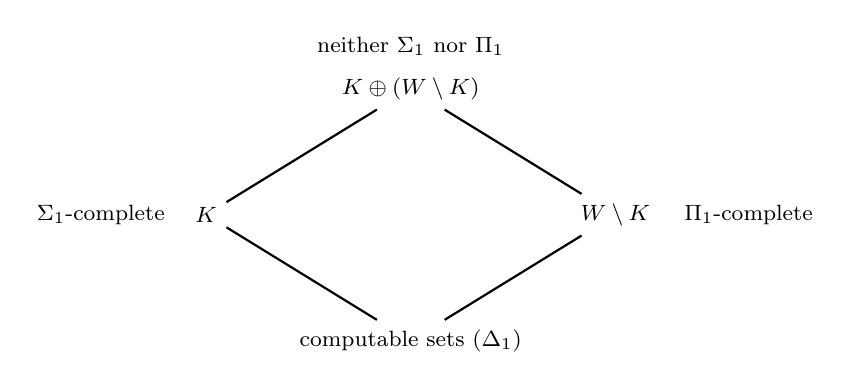
\begin{tikzpicture}[every node/.style={font=\footnotesize}]
	\node (bot) at (0,0) {computable sets ($\Delta_1$)};
	\node (k) at (-2.6,1.6) {$\KK$};
	\node (nk) at (2.6,1.6) {$\WW\setminus\KK$};
	\node (j) at (0,3.2) {$\KK \oplus (\WW\setminus\KK)$};
	\draw[thick] (bot) -- (k); \draw[thick] (bot) -- (nk);
	\draw[thick] (k) -- (j); \draw[thick] (nk) -- (j);
	\node[anchor=east] at (-3.0,1.6) {$\Sigma_1$-complete};
	\node[anchor=west] at (3.35,1.6) {$\Pi_1$-complete};
	\node[anchor=south] at (0,3.5) {neither $\Sigma_1$ nor $\Pi_1$};
\end{tikzpicture}
\end{center}

Iterating the construction produces infinitely many degrees, and in fact the structure of the many-one degrees is extremely rich; this is the subject of computability theory proper, which we do not pursue.

\subsection{Rice's Theorem}

The halting problem is unsolvable. Rice's theorem says, spectacularly, that \emph{every} non-trivial question about the behaviour of a program is unsolvable.

\begin{definition}
	Words $v, u$ are \vocab{weakly equivalent}, written $v \sim u$, if $W_v = W_u$; that is, if the machines they code halt on exactly the same inputs. A set $I \subseteq \WW$ is an \vocab{index set} if it is closed under weak equivalence.
\end{definition}

An index set is thus a set of programs specified purely by the \emph{function} they compute -- more precisely, by its domain -- rather than by any feature of the code. Index sets correspond exactly to properties of computably enumerable sets.

\begin{example}
	$\varnothing$ and $\WW$ are the trivial index sets. Others are
	\begin{align*}
		\Emp &= \{v \mid W_v = \varnothing\}, & \Fine &= \{v \mid W_v \text{ is finite}\}, \\
		\Inf &= \{v \mid W_v \text{ is infinite}\}, & \Tot &= \{v \mid W_v = \WW\}.
	\end{align*}
	The emptiness problem for programs is precisely $\Emp$.
\end{example}

The key construction is the following. Fix $w \in \WW$ and consider
$$g(u,v) = \begin{cases} f_{w,1}(v) & \text{if } u \in \KK, \\ \uparrow & \text{if } u \notin \KK.\end{cases}$$
This looks like an illegal case distinction, since membership of $\KK$ is not computable. But it \emph{is} computable, because we do not need to decide the case: on input $(u,v)$, run the machine coded by $u$ on input $u$; if and when it halts, run the machine coded by $w$ on input $v$ and return the answer. If $u \notin\KK$ the first phase never terminates, which produces exactly the divergence we want. This is a trick worth remembering: an uncomputable case distinction is harmless when the `false' branch is divergence.

By the $s$--$m$--$n$ theorem there is a total computable $h$ with $f_{h(u),1}(v) = g(u,v)$, so
$$W_{h(u)} = \begin{cases} W_w & u \in \KK, \\ \varnothing & u \notin \KK.\end{cases}$$

\begin{theorem}[Rice]\label{thm:rice}
	No non-trivial index set is computable.
\end{theorem}

\begin{proof}
	Let $I$ be an index set with $I \neq\varnothing,\WW$. Fix $e \in \WW$ with $W_e = \varnothing$ (for instance the code of a machine which never halts). Either $e \in I$ or not.

	\emph{Case $e \in I$.} Since $I \neq \WW$, choose $w \notin I$; then $W_w \neq \varnothing$, since $W_w = \varnothing$ would give $w \sim e$ and hence $w \in I$. Build $h$ as above from this $w$. If $u \in \KK$ then $W_{h(u)} = W_w$, so $h(u)\sim w$ and $h(u)\notin I$; if $u \notin\KK$ then $W_{h(u)} = \varnothing = W_e$, so $h(u)\sim e$ and $h(u)\in I$. Hence
	$$u \in \WW\setminus\KK \iff h(u) \in I,$$
	so $\WW\setminus\KK \leq_m I$ and $I$ is not computable.

	\emph{Case $e \notin I$.} Since $I \neq\varnothing$, choose $w \in I$; again $W_w \neq\varnothing$. With the same $h$: if $u \in \KK$ then $h(u)\sim w$ so $h(u)\in I$, and if $u\notin\KK$ then $h(u)\sim e$ so $h(u)\notin I$. Hence $\KK \leq_m I$, and again $I$ is not computable.
\end{proof}

\begin{remark}\label{rem:ricestronger}
	The proof gives more than the statement. If $e \in I$ then $\WW\setminus\KK \leq_m I$, so $I$ is not even computably enumerable. If $e \notin I$ then $\KK \leq_m I$, so $I$ is not $\Pi_1$; but this leaves open whether $I$ is computably enumerable.

	Applying this: $e \in \Emp$ and $e \in \Fine$, so neither $\Emp$ nor $\Fine$ is computably enumerable. On the other hand $e \notin\Inf$ and $e\notin\Tot$, so we obtain only $\KK\leq_m\Inf$ and $\KK\leq_m\Tot$.
\end{remark}

\begin{corollary}
	None of $\Emp, \Fine, \Inf, \Tot$ is computable.
\end{corollary}

\begin{theorem}
	$\Fine$ is neither $\Sigma_1$ nor $\Pi_1$.
\end{theorem}

\begin{proof}
	By Remark~\ref{rem:ricestronger}, $\WW\setminus\KK\leq_m\Fine$, so $\Fine$ is not $\Sigma_1$. For the other half we show $\KK\leq_m\Fine$. Consider
	$$g(w,v) = \begin{cases}\uparrow & \text{if } t_{w,1}(w,v) = a, \\ \eps & \text{otherwise},\end{cases}$$
	which is computable: compute the (total) truncated computation function and then either diverge or halt. By the $s$--$m$--$n$ theorem take total computable $h$ with $f_{h(w),1}(v) = g(w,v)$.

	If $w \in \KK$, let $v_0$ be the halting time of $f_{w,1}(w)$. Then $t_{w,1}(w,v) = a$ for all $v$ with $\#v > \#v_0$, so $f_{h(w),1}(v)\!\uparrow$ for all such $v$; hence $W_{h(w)}$ is contained in the finite set of $v$ with $\#v \leq \#v_0$, and is finite. So $h(w)\in\Fine$.

	If $w \notin\KK$ then $t_{w,1}(w,v) = \eps$ for every $v$, so $f_{h(w),1}$ is the total constant function $\eps$ and $W_{h(w)} = \WW$, which is infinite. So $h(w)\notin\Fine$.

	Hence $h$ is a reduction from $\KK$ to $\Fine$, and $\Fine$ is not $\Pi_1$.
\end{proof}

\begin{remark}
	By contrast, one can show that $\Emp \equiv_m \WW\setminus\KK$, so $\Emp$ is $\Pi_1$-complete, while $\Tot$ and $\Inf$ are, like $\Fine$, in neither class. The hierarchy of $\Sigma_n$ and $\Pi_n$ sets obtained by allowing $n$ alternating quantifiers -- the \emph{arithmetical hierarchy} -- is where these sets properly live.
\end{remark}

\subsection{Solvability of Decision Problems}\label{sec:solvability}

We can now return to the decision problems of Section~\ref{sec:cfl} with a precise definition in hand. Fix a coding of grammars such that every word $w$ codes a grammar $G_w$ and every grammar is $G_w$ for some $w$; this is arranged by decreeing that words which are not syntactically valid code some fixed trivial grammar. Then
\begin{enumerate}[label=(\roman*)]
	\item the word problem is the set $\{(w,v) \mid w \in \lang(G_v)\}$;
	\item the emptiness problem is the set $\{w \mid \lang(G_w) = \varnothing\}$;
	\item the equivalence problem is the set $\{(w,v)\mid \lang(G_w) = \lang(G_v)\}$;
\end{enumerate}
and each is \vocab{solvable} exactly when the corresponding set is computable.

\begin{theorem}
	The word problem for type $0$ grammars is unsolvable.
\end{theorem}

\begin{proof}
	Let $W = \{(w,v)\mid w \in \lang(G_v)\}$ and suppose it computable. Define
	$$f(w) = \begin{cases}\uparrow & w \in \lang(G_w), \\ a & w\notin\lang(G_w).\end{cases}$$
	Since $W$ is computable this is a legitimate case distinction, so $f$ is computable, and $\dom f$ is computably enumerable. By Theorem~\ref{thm:cetype0} there is a grammar $G$ with $\lang(G) = \dom f$, say $G = G_d$. But then
	$$d \in \lang(G_d) \iff d \in \dom f \iff f(d)\!\downarrow \iff d \notin \lang(G_d),$$
	a contradiction.
\end{proof}

\begin{corollary}
	The emptiness problem for type $0$ grammars is unsolvable.
\end{corollary}

\begin{proof}
	By Theorems~\ref{thm:type0ce} and~\ref{thm:cetype0}, $\{\lang(G_w) \mid w\in\WW\}$ is exactly the collection of computably enumerable sets, and translating between a grammar and a machine for the same language is effective in both directions. So the emptiness problem for grammars is many-one equivalent to $\Emp$, which is not computable by Rice's theorem.
\end{proof}

\begin{corollary}
	The equivalence problem for type $0$ grammars is unsolvable.
\end{corollary}

\begin{proof}
	Consider $\Eq = \{(w,v) \mid W_w = W_v\}$, and fix $e$ with $W_e = \varnothing$. The function $g(w) = (w,e)$ is total computable, and
	$$w \in \Emp \iff W_w = \varnothing = W_e \iff (w,e) \in \Eq,$$
	so $\Emp \leq_m \Eq$ and $\Eq$ is not computable. Translating to grammars as above gives the result.
\end{proof}

So all three of our problems, solvable for regular grammars and two of them for context-free grammars, become unsolvable at the top of the hierarchy.

\section{The Relationship Between the Language Classes}

We close by drawing the whole picture together. We have met the following classes of languages over a fixed alphabet $\Sigma$, in increasing order:
\begin{align*}
	\text{regular} \;\subseteq\; \text{context-free} &\;\subseteq\; \text{context-sensitive} \\
	&\;\subseteq\; \text{computable} \;\subseteq\; \text{computably enumerable} \;\subseteq\; \power(\WW).
\end{align*}

\begin{center}
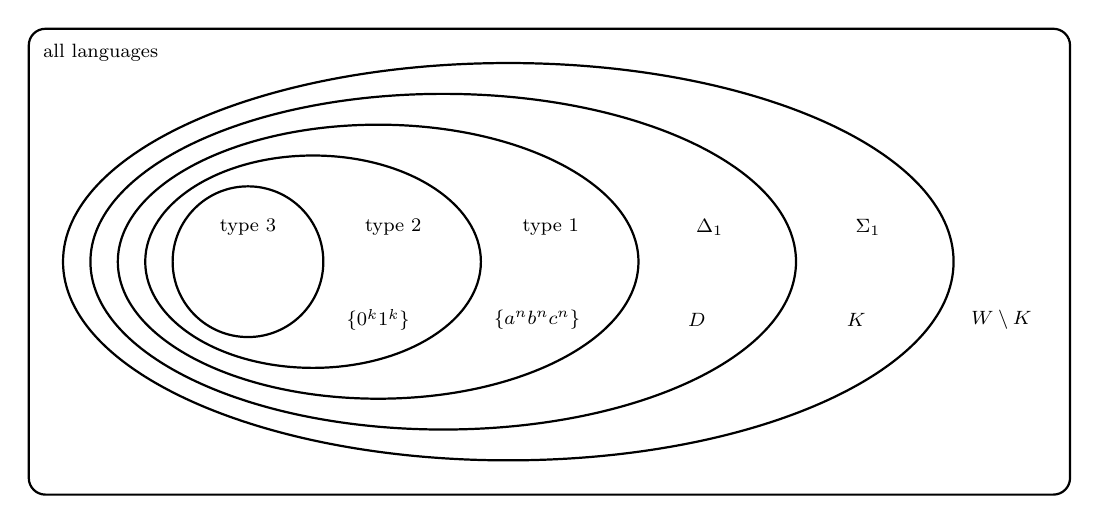
\begin{tikzpicture}[scale=0.87, transform shape,
	lbl/.style={font=\footnotesize, fill=white, inner sep=1.5pt}]
	\draw[blob] (-7.6,-3.4) rectangle (7.6,3.4);
	\draw[thick] (-0.6,0) ellipse (6.5 and 2.9);
	\draw[thick] (-1.55,0) ellipse (5.15 and 2.45);
	\draw[thick] (-2.5,0) ellipse (3.8 and 2.0);
	\draw[thick] (-3.45,0) ellipse (2.45 and 1.55);
	\draw[thick] (-4.4,0) ellipse (1.1 and 1.1);
	\node[lbl] at (-4.40,0.50) {type $3$};
	\node[lbl] at (-2.28,0.50) {type $2$};
	\node[lbl] at (0.02,0.50) {type $1$};
	\node[lbl] at (2.34,0.50) {$\Delta_1$};
	\node[lbl] at (4.65,0.50) {$\Sigma_1$};
	\node[lbl, anchor=west] at (-7.45,3.05) {all languages};
	\node[lbl] at (-2.50,-0.85) {$\{0^k1^k\}$};
	\node[lbl] at (-0.18,-0.85) {$\{a^nb^nc^n\}$};
	\node[lbl] at (2.15,-0.85) {$\mathbb{D}$};
	\node[lbl] at (4.48,-0.85) {$\KK$};
	\node[lbl] at (6.60,-0.85) {$\WW\setminus\KK$};
\end{tikzpicture}
\end{center}
Here type $3$, $2$, $1$ are the regular, context-free and context-sensitive languages, $\Delta_1$ the computable languages, and $\Sigma_1$ the computably enumerable languages, which are exactly the type $0$ languages.

Every inclusion is strict, and each strictness has been (or can be) witnessed:
\begin{itemize}
	\item $\{0^k1^k \mid k > 0\}$ is context-free but not regular, by the pumping lemma for regular languages (Example~\ref{ex:0k1knotregular}) or by Myhill--Nerode.
	\item $\{a^nb^nc^n \mid n > 0\}$ is context-sensitive but not context-free, by the pumping lemma for context-free languages (Example~\ref{ex:anbncn}).
	\item There is a computable language $\mathbb{D}$ which is not context-sensitive. Indeed, the context-sensitive grammars can be effectively enumerated as $G_0, G_1, \dots$, and the word problem for each is uniformly solvable by Corollary~\ref{cor:wordproblemsolvable}; so, listing the words of $\WW$ in shortlex order as $w_0, w_1, \dots$, the diagonal language
	$$\mathbb{D} = \{w_n \mid w_n \notin \lang(G_n)\}$$
	is computable but differs from every $\lang(G_n)$.
	\item $\KK$ is computably enumerable but not computable (Theorem~\ref{thm:halting}).
	\item $\WW\setminus\KK$ is a language which is not computably enumerable, hence not of the form $\lang(G)$ for any grammar at all (Corollary~\ref{cor:sigmanotcomplement}).
	\item Finally, there are uncountably many languages and only countably many grammars, so almost every language lies outside the outermost ellipse.
\end{itemize}

Closure properties and decision problems degrade as we ascend:
\begin{center}
	\begin{tabular}{l|ccccc}
		 & union & concat. & Kleene $+$ & intersection & complement \\\hline
		regular & yes & yes & yes & yes & yes \\
		context-free & yes & yes & yes & \emph{no} & \emph{no} \\
		context-sensitive & yes & yes & yes & yes & yes \\
		computable & yes & yes & yes & yes & yes \\
		computably enumerable & yes & yes & yes & yes & \emph{no}
	\end{tabular}
\end{center}
\begin{center}
	\begin{tabular}{l|ccc}
		 & word problem & emptiness & equivalence \\\hline
		regular & solvable & solvable & solvable \\
		context-free & solvable & solvable & \emph{unsolvable} \\
		context-sensitive & solvable & \emph{unsolvable} & \emph{unsolvable} \\
		computably enumerable & \emph{unsolvable} & \emph{unsolvable} & \emph{unsolvable}
	\end{tabular}
\end{center}

The context-free row is anomalous in the first table: it is the only class in the list failing to be closed under intersection, and we saw in Section~\ref{sec:cfl} that this is forced by the pushdown model, whose single stack cannot be duplicated. The last row of the second table is the content of Section~\ref{sec:solvability}.

There is a pleasing overall moral. Each class is characterised in two ways, by a grammar and by a machine:
\begin{center}
	\begin{tabular}{l|l|l}
		class & grammars & machines \\\hline
		regular & regular grammars & finite automata \\
		context-free & context-free grammars & pushdown automata \\
		context-sensitive & noncontracting grammars & linear bounded automata \\
		computably enumerable & arbitrary grammars & register (or Turing) machines
	\end{tabular}
\end{center}
and the amount of memory available to the machine -- none, a stack, a tape of length proportional to the input, an unbounded tape -- is exactly what determines the class. That is the shape of the subject: a hierarchy of languages, a matching hierarchy of machines, and at the top, an unavoidable wall of undecidability.

\end{document}
